
\documentclass[12pt]{report}
\usepackage{jrl_thesis}
\usepackage{fancyheadings}
\usepackage{natbib}
\usepackage{setspace}               % this package defines the spacing of your thesis and should be included
             % your information goes here
\usepackage{titlesec}
\usepackage{hyperref}
\usepackage[pdftex]{graphicx}
\usepackage{subcaption}
\usepackage{mathtools}
\usepackage{amsmath}
\usepackage{caption}
\usepackage{verbatim}
\usepackage{cleveref}
\usepackage{listings}
%\usepackage[framed,numbered,autolinebreaks,useliterate]{mcode}
\usepackage{pdfpages}

%\usepackage{amssymb}
%\usepackage[colorinlistoftodos]{todonotes}
%\usepackage{xcolor}
%\usepackage{fancyhdr}


\graphicspath{{./figures/}}
\titleclass{\subsubsubsection}{straight}[\subsection]

\newcounter{subsubsubsection}[subsubsection]
\renewcommand\thesubsubsubsection{\thesubsubsection.\arabic{subsubsubsection}}
\renewcommand\theparagraph{\thesubsubsubsection.\arabic{paragraph}} % optional; useful if paragraphs are to be numbered

\titleformat{\subsubsubsection}
  {\normalfont\normalsize\bfseries}{\thesubsubsubsection}{1em}{}
\titlespacing*{\subsubsubsection}
{0pt}{3.25ex plus 1ex minus .2ex}{1.5ex plus .2ex}

\makeatletter
\renewcommand\paragraph{\@startsection{paragraph}{5}{\z@}%
  {3.25ex \@plus1ex \@minus.2ex}%
  {-1em}%
  {\normalfont\normalsize\bfseries}}
\renewcommand\subparagraph{\@startsection{subparagraph}{6}{\parindent}%
  {3.25ex \@plus1ex \@minus .2ex}%
  {-1em}%
  {\normalfont\normalsize\bfseries}}
\def\toclevel@subsubsubsection{4}
\def\toclevel@paragraph{5}
\def\toclevel@paragraph{6}
\def\l@subsubsubsection{\@dottedtocline{4}{7em}{4em}}
\def\l@paragraph{\@dottedtocline{5}{10em}{5em}}
\def\l@subparagraph{\@dottedtocline{6}{14em}{6em}}
\makeatother

\setcounter{secnumdepth}{4}
\setcounter{tocdepth}{4}
% add all other packages that you need to use here.

% ********************************
\begin{document}
\beforepreface                      % command to create the parts of your thesis that come before the preface like title and etc.
\thispagestyle{empty}
\null\vfill
\begin{center}
%\textbf{Dedications}
%\linebreak
\textsl{Dedication}
\end{center}
\vfill

\prefacesection{Lay Abstract}

\textbf{Non-technical abstractt. Is this needed?}


\title{Thesis Title}
\author{Name}

\prevdegreeone{Previous Degree}

\prevdegreetwo{Second previous degree if any}

\submitdate{Submit date}

\copyrightyear{copyright year}

\principaladviser{Dr. Ian C. Bruce}
  

  \include{abstr}
  \include{acknowledgements}
  \prefacesection{Notation and abbreviations}

\textbf{Notation1}		Definition\\
\textbf{Notation2}		Definition\\






\afterpreface                      % command to create the parts of your thesis that come after your preface like contents and etc.

  \chapter{Introduction and Literature Review}

\section{Introduction}
                  % the first chapter
        \setcounter{figure}{0}
        \setcounter{equation}{0}
        \setcounter{table}{0}

  % add other chapters go here. don't forget to reset the counters each time!

\chapter{De-Reverberation Literature Review}

Intro: Overview of techniques to be discussed (breakdown of categories)



\section{Reverberation Suppression}
\subsection{Beamforming}
\subsection{Linear Prediction Residual Enhancement}
\subsection{Statistical Methods}

\section{Reverberation Cancellation}
\subsection{Invertibility of Room Impulse Response} \label{RIR_Invertibility}

To perfectly cancel reverberation, an equalizer filter must be designed such that the result of cascading the RIR with the equalizer is an impulse. I.e., for a RIR $g(n)$ and an equalizer $h(n)$, the ideal equalized impulse response (EIR) $d(n)$  is

\begin{equation} 
d(n)=g(n)*h(n)=\delta(n)
\end{equation}

\noindent
Which in the Z-transform domain is

\begin{eqnarray}
D(z)=G(z)H(z)=1	\\
H(z)=\frac{1}{G(z)}
\end{eqnarray}

Therefore, the ideal equalizer would be the inverse of the RTF. However \cite{neely1979invertibility} showed that RTFs are typically non-minimum phase, making the realization of a causal and stable inverse impossible. The non-minimum phase nature of RTFs is related to the acoustics of the room and the positioning of the sound source and listener. In particular \cite{neely1979invertibility} showed that for synthetic room acoustics, there is a threshold of wall reflectivities over which the RTF becomes non-minimum phase. Similarly, it was shown that by increasing room size, increasing source/listener separation and placing the source and listener at more symmetrical positions, the RTF was more likely to be non-minimum phase. In typical conditions (e.g., an office room), these conditions for a minimum phase RTF are not met. From a time-domain perspective, to be minimum phase the first non-zero sample of the RIR (i.e., the direct sound or first arriving reflection when there is no direct sound) must be larger than the later reflections, and the RIR must decay rapidly. Even in rooms with relatively short reverberation times (e.g., approximately \qty{200}{\milli\second}), the decay is not short enough to produce a minimum phase RTF.

For typical RIRs, the theoretical inverse systems have very long impulse responses, often being infinite length (IIR) or even two-sided IIR. This can be explained largely by RTFs having strong notches which appear as zeros very close to or on the unit circle. The resulting inverse filter therefore has poles very close to the unit circle resulting in very long decay. For this reason, equalizer filter structure selection is an important factor in performance. While a FIR equalizer will always be an approximation of the true IIR inverse, even for a minimum phase system, reasonable performance can be acheived for a long enough FIR filter. On the other hand, an IIR filter can acheive perfect equalization for minimum phase systems and often requires lower complexity than its FIR counterpart.

Additionally, perfect equalization of strong spectral notches is undesirable in practice since the equalizer will include strong peaks which will substantially amplify noise. In the extreme case, this narrowband noise resonance was reported by \cite{neely1979invertibility} as an audible chime-like artifact. Furthermore, if the RTF has zeros exactly on the unit circle, this results in complete loss of content at that frequency, making it unrecoverable even in absense of background noise.

 For maximum phase RTFs with zeros strictly outside the unit circle, the inverse systems are one-sided IIR, and are either causal unstable (i.e., right-sided) or acausal stable (i.e., left-sided). For mixed-phase RTFs, the inverse system is always two-sided IIR regardless of stability. Since a practical filter must be stable, the ideal equalizer would have to be acausal or two-sided. Infinitely left-sided filters are not implementable in realtime since they would require prior knowledge of infinite future data. However, it is theoretically possible to implement an infinitely left-sided filter offline, by performing two filtering operations: one in forward-time (i.e., causal filtering) and one in reverse-time (i.e., acausal filtering) \citep{kormylo1974twopass}. However, \cite{treitel1966design} showed that by introducing a modeling delay $D$ to the desired EIR (i.e., equalizing to a delayed impulse) enables partial implementation of the left side of the ideal system inverse. I.e., 

\begin{eqnarray}
	d(n)=g(n)*h(n)=\delta(n-D) \\
	D(z)=G(z)H(z)=z^{-D}	\\
	H(z)=\frac{z^{-D}}{G(z)}
\end{eqnarray}

This has the effect of shifting some of the acausal portion of the stable inverse filter to causal side, and greatly improve equalizer performance. Increasing modeling delay always improves equalizer performance, but equalization is still approximate since perfect equalization would in general require infinite delay. Additionally, introduction of signficant delay can reduce user experience, and can result in audible artifacts due to equalizer error, i.e., pre-ringing and pre-echo, \citep{brannmark2009spatially}. The design of an effective equalizer must carefully manage the tradeoff between reverberation cancellation and these other adverse perceptual effects.

Another challenge in the design of a practical room response equalizer arises from the highly non-stationary nature of the RTF, both in space and time. \cite{mourjopoulos1985variation} showed that RIR varies signficantly with respect to loudspeaker and microphone location and as a result an equalizer only applies exactly within a very small spatial region (i.e., the equalized zone). It was shown that the equalized zone is smaller than the interaural distance at high frequencies. Movement of the sound source, listener and objects in the room, as well as temperature variations result in variation of the RIR over time \citep{omura1999compensating}. For similar reasons, it has been shown that small errors in the equalizer (e.g., due to errors in the model of the RIR and due to computational error) result in significant worsening of equalizer performance, often resulting in making the effect of reverberation worse. To make equalizers more robust to variation, several design approaches have been proposed which attempt to equalize the room response at multiple locations simultaneously \citep{elliott1989multiple, haneda1997multiple}. This reduces equalizer performance at each individual location, but results in a more stable solution.

\textbf{Ill-Conditioning: Add to next section (More on the context of solving for the inverse)}

In the context of dereverberation for speech perception, it is also important to consider the perceptual benefit of early reflections which provide an effective SNR boost as previously described. Several authors have proposed modifications to existing equalizer design methods which maintain early reflections \citep{karjalainen2006equalization, maamar2006partial, mei2009room}. These appraoches are referred to as room response reshaping, channel shortening or partial equalization.

It is also important to make a distinction between the problem of equalizing the RTF at a certain location by preprocessing the signal sent to a spatially separated loudspeaker, and equalizing the RTF locally at the microphone (e.g., on a hearing aid). \textbf{In the context of loudspeaker room equalization...}

\subsection{Single Channel Room Response Equalization}

\subsubsection{Homomorphic Approaches to Room Response Equalization}

The first approach to equalization of a non-minimum phase RTF, proposed by \cite{neely1979invertibility}, decomposed the RTF, $G(z)$, into it's minimum phase and allpass mixed phase components, 

\begin{equation}
	G(z)=G_{\mathrm{min}}(z)G_{\mathrm{allpass}}(z)
\end{equation}

\noindent
and designed an equalizer, $H(z)$, by inverting only the minimum-phase component. 

\begin{equation}
	H(z)=\frac{1}{G_{\mathrm{min}}(z)}
\end{equation}

\noindent
The resulting EIR, $D(z)$, is

\begin{equation}
	D(z)=G(z)H(z)=G_{\mathrm{allpass}}(z)
\end{equation}

The authors modeled the RTF with a FIR RIR, and estimated the minimum phase component by computing the cepstrum (i.e., the real cepstrum) of the RIR, and flipping/adding the negative quefrency cepstral coefficients with the positive quefrency coefficients. The processed cepstrum is returned to the time domain by an inverse complex cepstrum transformation. Since the real cepstrum represents a magnitude response (i.e., zero phase) and a right-sided complex cepstrum represents a minimum phase sequence, the resulting time-domain sequence represents the equivalent minimum phase representation of the original RIR. This process uses the inverse DFT to compute the equalizer, therefore the DFT size must be large enough to minimize distortions due to time domain aliasing. 

This approach perfectly equalizes the magnitude response of the channel, but the excess phase response of the allpass component, $G_{\mathrm{allpass}}(z)$,  and as such is referred to as magnitude equalization or excess phase equalization. The residual phase is visible in the group delay, which is flat except for significant deviations near the maximum phase zeros. However it has been shown that the excess phase in the allpass component contain most of the reverberant energy and as such is not perceptually negligible \citep{johansen1996excess}. In other words, the allpass component is responsible for the temporal smearing of reverberation. The significant peceptual impact of this can be explained by the fact that the short term frequency spectral analysis performed by the human auditory system is sensitive to excess phase.

Perfect equalization to a delay is theoreticallys possible by convolving the output of the magnitude equalizer through a time-reversed version of the all-pass component (i.e., matched filter). However, for an IIR filter this will impose infinite delay, and is equivalent to the modeling delay discussed in the previous section.

The shortcomings of the excess phase equalizer proposed by \cite{neely1979invertibility} motivates the need for an alternative form of partial equalization which emphasizes the importance of phase equalization, i.e., makes trade off between magnitude and phase equalization. \cite{radlovic2000nonminimum} and subsequently \cite{maamar2006partial}, proposed iteratively flattening the magnitude response while monitoring the excess phase response as a means to trade off the two.

\subsubsection{Linear Prediction Approaches to Room Response Equalization}

An alternative method for coming up with an estimate of the minimum phase component discussed in the previous section is accomplished via linear prediction. This idea has been explored by several authors, such as \cite{mourjopoulos1991pole} and \cite{haneda1997multiple}. In this approach, the RTF is modeled as an all-pole filter, and a FIR equalizer is designed by minimization of the error $e(n)$ between the actual channel RIR $g(n)$ and a predicted autoregressive model of the RIR $\hat{g}(n)$. I.e.,

\begin{eqnarray}
	e(n)= g(n) - \hat{g}(n) \\
	=  g(n) - \sum_{k=1}^{p}\alpha_k g(n-k) \\
	\boldsymbol{\alpha}=\begin{bmatrix} \alpha_1 & \alpha_2 & \dots & \alpha_p \end{bmatrix} = \underset{\boldsymbol{\alpha}}{\arg\min}\;e(n)
\end{eqnarray}

By using the autocorrelation method for linear prediction, the minimum phase component of the RTF is estimated and is equalized by the prediction error filter. Since poles ring longer than zeros, the method also generally produces a lower order model of the RTF peaks, and therefore also produces lower order equalizer. Compared to the FIR model in the previous section all-pole modeling of the RTF is more perceptually relevant since it does a better job of modeling high energy spectral peaks \citep{toole1988modification}. Additionally, by focusing less on modeling the RTF notches, the all-pole model is less sensitive to their high spatial/time variance  \citep{mourjopoulos1985variation}, which is especially impactful on avoiding over amplification of noise at the frequencies of deep spectral notches (i.e., the tonal artifacts reported by \cite{neely1979invertibility}). The linear prediction approach also enables usage of the computationally efficient Levinson Durbin algorithm, and is a more numerically stable technique due shorter equalizer filter lengths and avoidance of temporal aliasing due to the DFT used in cepstral analysis. However, unlike the homomorphic method which separately predicts the minimum phase and all-pass components, linear prediction only predicts the minimum phase component. Therefore to equalize the excess phase (e.g., via a matched filter), the excess all-pass phase response must be estimated by other means. 

\textbf{what about covariance approach to LPC?}

\subsubsection{Frequency Domain Approaches to Room Response Equalization}

Perhaps the most obvious approach to RTF inversion is to take the DFT of the RIR, compute its inverse, and then thake the inverse DFT to compute the FIR equalizer coefficients. Authors such as \cite{kulp1988digital} have explored this topic, and the challenges and design considerations associated with it. Most importantly, DFT size must be carefully selected to minimize distortions due to temporal aliasing. Since the inverse of RTFs is generally infinite in length, aliasing cannot be completely avoided, but the amount of aliased energy can be reduced. Many authors have suggested RIR pre-processing techniques to further mitigate this issue, such as applying a window function to emphasize key parts of the RIR \citep{kulp1988digital} and using regularization to reduce depth of spectral notches with the goal of reducing noise amplification \citep{bean1989loudspeaker, kirkeby1996fast}. As in preivous methods, delay can be introduced to partially shift the acausal portion of the RTF inverse to the causal side. Unlike the minimum phase equalization method discussed already, the frequency domain inversion directly computes the inverse to the full RTF and in absense of RIR pre-processing is not constrained. As such, it has been shown that with sufficient delay and a large enough DFT size, perfect equalization of a non-minimum phase system can be effectively acheived. Computing the inverse filter in the frequency domain additionally makes it possible to perform the deconvolution filtering process in the frequency domain, i.e., using an FFT to perform fast convolution. However, this approach is still always approximate, and is still susceptible to the issues of RTF variation in space and time, and artifacts such as noise amplification, pre-ringing and pre-echo.

\subsubsection{Least Squares Optimization Approaches to Room Response Equalization}

To better account for the importance of the all-pass component in terms of reverberant energy, several authors (e.g., \cite{clarkson1985spectral}) have proposed the usage of least squares optimization to minimize the error energy between the desired EIR $\tilde{y}(n)$ and the acheived EIR $y(n)=h(n)*g(n)$.  The desired EIR is set to a delayed impulse, i.e., $\tilde{y}(n)=\delta(n-d)$ to enable partial cancelation of the acausal portion of the ideal RTF inverse. The modeling error is thus

\begin{equation}
	e(n) = \tilde{y}(n)  - y(n) = \delta(n-d) - h(n)*g(n)
\end{equation}

\noindent
and the equalizer is designed to minimize the modeling error enery, i.e.,

\begin{eqnarray}
I = \sum_{n=0}^{N}e^2(n) \\
h(n) = \underset{h(n)}{\arg\min}\;I
\end{eqnarray}

\noindent
which is solved via the well known normal equations already discussed.

As previously mentioned, the selection of the delay is represents a trade off between equalizer performance, and undesirable perceptual effects sucha as delay and pre-ringing/pre-echo. Several authors have proposed methods for determining the optimal delay in this regard \citep{clarkson1985spectral, ford1978optimum}.

Where the previously discussed approaches come up with a specific deterministic minimum-phase approximation of the non-minimum phase inverse, this approach uses least squares to directly minimize the modeling error, without constraining the implications on the magnitude and phase responses. The least squares approach has been shown to outperform the minimum-phase qualization in terms of excess reverberant energy \citep{mourjopoulos1982comparative}.

\textbf{add proof that EQ of FIR channel with FIR filter is numerically impossibhle (matrix inversion dimensions dont work -- see note on paper)}

\subsection{Multiple Input-Output Inverse Theorem (MINT)}

In their seminal paper \cite{miyoshi1986inverse} proposed the multiple-input/output inverse theorem (MINT), which performed RTF equalization by exploiting multiple acoustic channels, i.e., multiple spatially separated loudspeakers and/or microphones. Two separate forms for MINT equalizers were presented, and their applications were described as sound reproduction and dereverberation (figure).

(figure sound reproduction vs dereverberation)

Sound reproduction describes a multiple-input single-output (MISO) system, where each loudspeaker signal is pre-processed with a unique FIR equalizer so as to equalize the RTF at a certain location in the room. Dereverberation describes a single-input multiple-output (SIMO) system where the microphone signals are filtered and summed, with the intention obtaining a clean signal that can be played back elsewhere (e.g., a hearing aid loudspeaker inside the ear canal).

In the SIMO dereverberation case, which is relevant to this thesis, the solution can be derived as follows. Let $g_i(n)$ be the length-$n$ FIR RIR corresponding to acoustic RTF between the source loudspeaker and microphone $i$. Let $h_i(n)$ be the length-$m$ FIR equalizer applied to microphone $i$ before summation with the other channels. 

\begin{eqnarray}
	G_i(z) = Z\{g_i(n)\} = \sum_{k=0}^{n-1}g_i(k)z^{-k} \\
	H_i(z) = Z\{h_i(n)\} = \sum_{k=0}^{m-1}h_i(k)z^{-k} \\
\end{eqnarray}

The inverse filtering problem can be stated in matrix form as

\begin{eqnarray}
	G\boldsymbol{h}=\boldsymbol{d} \label{eq:MINT_problem} \\
	%
	G\boldsymbol{h} =
	\begin{bmatrix}
		G_1 & G_2 & \dots& G_N
	\end{bmatrix} 
	\begin{bmatrix}
		\boldsymbol{h_1} \\
		\boldsymbol{h_2} \\
		\vdots \\
		\boldsymbol{h_N} \\
	\end{bmatrix}
	=
	\begin{bmatrix}
		d(0) \\
		d(1) \\
		\vdots \\
		d(m+n-2) \\
	\end{bmatrix} 
	=
	\boldsymbol{d}
\end{eqnarray}

\noindent
Where $\boldsymbol{h_i}$ is the vector form of the FIR equalizer applied to microphone $i$, i.e.,

\begin{eqnarray}
	\boldsymbol{h_i} = 
		\begin{bmatrix}
			h_i(0) & h_i(1) & \dots & h_i(m-1)
		\end{bmatrix}^T
\end{eqnarray}

\noindent
and $G_i$ is the filter matrix (i.e., the Sylvester matrix) corresponding to the convolution of $g_i(n)$ with $h_i(n)$, i.e.,

\begin{eqnarray}
	G_i = 
	\begin{bmatrix} 
		g_i(0)     & 0           & 0              & \dots    & 0  \\
		g_i(1)     & g_i(0)    & 0              & \dots    & 0  \\
		g_i(2)    & g_i(1)     & g_i(0)      & \dots    & 0  \\
		\vdots    & \vdots    & \vdots     & \ddots & \vdots  \\
		g_i(n-1) & g_i(n-2) & g_i(n-3) & \dots   & 0 \\
		0            & g_i(n-1)  & g_i(n-2) & \dots   & 0 \\
		0            & 0             & g_i(n-1
		111) & \dots   & 0 \\
		\vdots    & \vdots    & \vdots     & \ddots & \vdots  \\
		0            & 0             & 0             & \dots   & g_i(n-1) \\
	\end{bmatrix} 
	\in \mathbb{R}^{(m+n-1)\times m}
\end{eqnarray}

\noindent
To acheive perfect zero-delay equalization, the desired EIR should be $d(n)=\delta(n)$, and therefore

\begin{equation}
	\boldsymbol{d} =
		\begin{bmatrix}
			1 & 0 & \dots & 0
		\end{bmatrix}^T
\end{equation}

Since $G \in \mathbb{R}^{(m+n-1)\times Nm}$, equation \ref{eq:MINT_problem} represents a problem with $m+n-1$ equations and $Nm$ variables. A perfect solution exists provided $G$ is invertible, which requires that it is square and full rank. For $G$ to be square, that the equalizer filter length, $m$, must be

\begin{equation}
	m = \frac{n-1}{N-1}
\end{equation}

\noindent
Provided $G$ is full rank, the MINT can be computed as

\begin{equation}
	\boldsymbol{h} = G^{-1}\boldsymbol{d}
\end{equation}

For $m < \frac{n-1}{N-1}$, the problem is overdetermined and no perfect solution exists, i.e., it can only be solved by least squares. However, for $m > \frac{n-1}{N-1}$, the problem is underdetermined and therefore has infinite perfect solutions provided its rank is greater than or equal to the number of columns/unknowns. In this case the pseudo-inverse can be used to select the minimum norm solution. I.e.,

\begin{equation}
	\boldsymbol{h} = G^+\boldsymbol{d} = G^T(GG^T)^{-1}\boldsymbol{d}
\end{equation}

\textbf{Confirm that this form of the psuedo inverse is required for solving an underdetermined system, and is different from the other form which is used for solving an overdetermined system (i.e., least squares)}

 Therefore, for the SIMO dereverberation case, the equalizer filter length, $m$ is required to be

\begin{equation}
	m >= \frac{n-1}{N-1}
\end{equation}

\noindent
where $m$ is the length of the individual FIR equalizers, $n$ is the length of the individual FIR channels, and $N$ is the number of microphones. Note that although the individual FIR channels are not necessarily the same length, they can be zero padded to the longest length.

Equivalently, for the MISO sound reproduction case, the equalizer filter length requirement was shown to be

\begin{equation}
	m >= \frac{n-1}{M-1}
\end{equation}

\noindent
where $M$ is the number of loudspeakers.


 \cite{miyoshi1986inverse} proved that in order to be invertible (i.e., in order for $G$ to be full rank), there could not be any zeros that were common to all RTFs. It was therefore shown that a MINT equalizer can achieve perfect zero-delay equalization, even when the individual RTFs are non-minimum phase, provided the equalizer filter lengths are sufficiently long and the individual RTFs do not have common zeros anywhere in the z-plane. This result is different from single channel methods which only approach perfect equalization of non-minimum phase channels as the modeling delay approaches infinity. 
 
 It is interesting to note that FIR channels would inheritly have inverse filters that are all-pole and therefore IIR. Single channel FIR equalization of a FIR channel will thus always be approximate, even if the channel is minimum phase. This makes sense intuitively, but \cite{miyoshi1986inverse} also proved this numerically by demonstrating that the matrix formulation of the single channel equalization problem is always overdetermined regardless of equalizer filter length. Remarkably, the MINT can acheive perfect equalization of a FIR channel with individual FIR equalizer filters that are shorter in length than the FIR channels. It is important to remember that real RTFs are not generally speaking FIR, so the MINT is still approximate. However, for a sufficiently long FIR measurement of the true RIR, the residual reflections may be considered negligible.The MINT was proven to greatly outperform the single channel least squares equalization method, acheiving more than \qty{40}{dB} additional reverberation attenuation accross all frequencies.
 
In an extended discussion of the MINT,  \cite{miyoshi1988inverse} explored the MIMO case for sound reproduction as shown in (figure)

(figure MIMO MINT)

They proved that it is possible to perform sound reproduction at $N$ listening positions using $M$ loudspeakers provided the channels had no common zeros,

\begin{equation}
	M > N
\end{equation}

and

\begin{equation}
	m >= \frac{N(n-1)}{M-N}
\end{equation}

In an extension of the MINT, \cite{nakajima1997sound} proposed the indefinite MINT filter (IMF) which exploits the additional degrees of freedom gained when the FIR equalizer length $m$ is strictly greater than its minimum required length. In this underdetermined case, there are infinite solutions. While the classical MINT recommended using the pseudo inverse to compute the minimum norm solution, IMF makes use of the additional degrees to equalize nearby points. This has the effect of expanding the equalized zone and improving robustness to spatial variation of the RTF.


\subsection{Blind Deconvolution Problem}

The RTF equalization approaches discussed in the previous section were reliant on having prior knowledge of the RIR (e.g., by measurement). However, typically in the context of dereverberation, the RIR is not known and must be estimated by other means. The approaches to estimation of a unknown linear system can be divided into supervised methods (i.e., trained/supervised deconvolution) and unsupervised methods (i.e., blind/unsupervised deconvolution).

\subsubsection{The Wiener Filter (Supervised Optimal Filtering)}

Traditional supervised optimal filtering is formulated as the selection of a filter $H(z)$ which, for a known input sequence $x(n)$, produces a output $y(n)$ that is optimally close (in a mean-squared error sense) to a desired/reference signal $d(n)$. I.e., the goal is to design $H(z)$ such that the energy in the error signal $e(n) = d(n)-y(n)$ is minimized. 

\begin{figure}[H]
	\includegraphics[scale=0.4]{WienerFilter}
	\centering
	\caption{Block diagram for supervised optimal filtering, which attempts to produce a desired output, $d(n)$, from a known input, $x(n)$}
	\label{fig:WienerFilterProblem}
\end{figure}

When applied to system equalization (e.g., RTF equalization), as depicted in Figure \ref{fig:supervised_inverse_filter}, the desired/reference signal is the input to the unknown system, i.e., $d(n)=s(n)$, and input to the equalizer filter, $H(z)$, is the output of the unknown system, i.e., $x(n)=m(n)$. 

\begin{figure}[H]
	\includegraphics[scale=0.35]{supervised_inverse_filter}
	\centering
	\caption{Block diagram for supervised inverse filtering / equalization, which attempts to produce reproduce the known input, $s(n)$, to an unknown system $G(z)$, from the measured system output, $m(n)$, using a filter, $H(z)$}
	\label{fig:supervised_inverse_filter}
\end{figure}


The derivation for this optimal solution, originally proposed by \cite{wiener1949extrapolation}, is performed in a stochastic framework using expectations for computing mean-squared error. The resulting solution is referred to as the Wiener filter. Considering a length-$N$ FIR filter, $H(z)=\sum_{k=0}^{N-1}h_k z^{-k}$, this is mathematically formulated as

\begin{eqnarray}
	\boldsymbol{x}(n) = 
	\begin{bmatrix}
		x(n) & x(n-1) & \dots & x(n-N+1)
	\end{bmatrix}^T \\
	%
	\boldsymbol{h} = 
	\begin{bmatrix}
		h_0^* & h_1^* & \dots & h_{N-1}^*
	\end{bmatrix}^T \\
	%
	e(n)=d(n) - y(n) = d(n) - \boldsymbol{h}^H\boldsymbol{x}(n) \\
	%
	J(\boldsymbol{h}) = E\left[ \left| e(n) \right|^2 \right] = E\left[e(n)e^H(n)\right] \\
	%
	J(\boldsymbol{h}) = E\left[
	\left(d(n) - \boldsymbol{h}^H\boldsymbol{x}(n)\right)
	\left(d(n) - \boldsymbol{h}^H\boldsymbol{x}(n)\right)^H
	\right] \label{eq:wiener_cost_fn_0} \\
	% 
	J(\boldsymbol{h}) = \sigma_d^2 - \boldsymbol{h}^H\boldsymbol{p} - \boldsymbol{h}^T\boldsymbol{p}^*+\boldsymbol{h}^H R \boldsymbol{h} \label{eq:wiener_quadratic}
\end{eqnarray}

\noindent
Where $\boldsymbol{p} = E \left[ \boldsymbol{x}(n)d^*(n) \right]$ is the cross-correlation vector between the input process and the desired/reference process, and $R = E \left[ \boldsymbol{x}(n)\boldsymbol{x}^H (n) \right]$ is the autocorrelation matrix of the input process.

Since the highest-order factor in Equation \ref{eq:wiener_quadratic}, i.e., $\boldsymbol{h}^H R \boldsymbol{h}$ is a quadratic form and the autocorrelation matrix $R$ is Hermitian positive semidefinite (assuming the input process is stationary), $J(\boldsymbol{h})$ represents a quadratic bowl in $N+1$ dimensions with exactly one global minimum. This minimum can be found by taking the derivative of the cost function and setting it equal to zero. I.e.,


\begin{eqnarray}
	%
	\frac{\partial J(\boldsymbol{h})}{\partial \boldsymbol{h}^*}=0 \\
	%
	R \boldsymbol{h} = \boldsymbol{p} \label{eq:wiener_hopf}
\end{eqnarray}

Equation \ref{eq:wiener_hopf} is referred to as the Wiener-Hopf equation and can be solved by any number of methods for solving systems of linear equations. This equation can also be viewed as a stochastic extension of the LS normal equations, and equivalently the Yule-Walker equations in linear prediction. I.e., the Wiener filter is optimal for known stationary processes, whereas the LS normal equations produce a filter that is optimal for a known set of data. 

In practice the statistical correlation functions that make up $\boldsymbol{p}$ and $R$ in the Wiener-Hopf equations must be estimated from a finite set of data, and given certain short-term estimation techniques, the Wiener-Hopf equations become identical to the LS normal equations.

The conditioning of the Wiener-Hopf equation is dictated by the eigenvalue spread of the autocorrelation matrix, $R$, which has been shown to be correlated to the dynamic range of the input spectrum (i.e., the “peakiness”). When the input process is white, the eigenvalue spread is equal to 1, and the autocorrelation matrix is the identity matrix. When the input sequence is coloured, the non-zero off-diagonal autocorrelation values result in a larger eigenvalue spread (i.e., higher condition number), which can lead to a less numerically stable solution.

In practice there is always additional sensor noise present which interferes with the measured input, $x(n)$, and/or error signal, $e(n)$. This interference leads to additional misadjustments of the final solution due to distortions in the autocorrelation matrix.

The Wiener filter has also been extended to the optimal derivation of an IIR filter (i.e., the unconstrained Wiener filter), which results in the following frequency domain solution.

\begin{equation}
	\boldsymbol{h}(e^{j\omega}) = \frac{\Phi_{dx}(e^{j\omega})}{\Phi_{xx}(e^{j\omega})}
\end{equation}

\noindent
Where $\Phi_{dx}(e^{j\omega})$ is the cross-PSD of $d(n)$ and $x(n)$, and $\Phi_{xx}(e^{j\omega})$ is the PSD of $x(n)$.

The Wiener filter and all resulting adaptive extensions can be applied to both transversal filters (as described above) and linear combiners (e.g., beamforming). 

\subsubsection{Supervised Adaptive Filtering}

To allow tracking of time-varying systems, adaptive algorithms have been proposed which aim to converge on the Wiener filter. Adaptive filtering theory leverages the fact that the MSE cost function forms a quadratic error surface, and generally performs some form of gradient descent to make iterative steps towards the optimal solution. A detailed discussion of the details of adaptive filtering theory can be found in \cite{farhang2013adaptive}, but an overview of the most common algorithms will be provided below.

The steepest descent algorithm (SD) estimates the gradient,

\begin{equation}
	\bold{\nabla} J(\boldsymbol{h}) = 
	\frac{\partial J(\boldsymbol{h})}{\partial \boldsymbol{h}^*} = \frac{\partial E\left[e(n)e^H(n)\right]}{\partial \boldsymbol{h}^*} \\
\end{equation}


\noindent
of the MSE error surface and steps in the direction opposite to it. The shape of the error surface is dictated by the eigenvalue spread of the autocorrelation matrix for the input sequence, and therefore also the peakiness of the input spectrum. For a white input spectrum, the equal-MSE contours for the error surface are circular, and the negative gradient points directly towards the optimal solution. For more coloured/peaky spectra, the equal-MSE contours of the error surface become elongated, resulting in a negative gradient which does not point directly towards the optimal solution. The Newton descent (ND) algorithm modified SD by deriving the optimal vector-valued step such that the direction of iteration always points directly to the optimal solution regardless of eigenvalue spread

Both SD and ND require estimation of the autocorrelation matrix, $R$, and the cross-correlation vector, $p$. This is computationally expensive, and also it is common for the desired/reference process to be unknown (i.e., only the error sequence is known), making the cross-correlation vector, $p$, impossible to estimate. This motivated the usage of the stochastic gradient which is computed solely based on the measured error sequence. The stochastic gradient, defined as

\begin{equation}
	\frac{\partial \left(e(n)e^H(n)\right)}{\partial \boldsymbol{h}^*} = - \boldsymbol{x}(n)e^*(n) \\
\end{equation},

\noindent
represents an instaneous stochastic estimate of the true gradient, $ \frac{\partial E\left[e(n)e^H(n)\right]}{\partial \boldsymbol{h}^*} $.

The commonly used least-mean-squares (LMS) algorithm, steps in the direction of the negative stochastic gradient, using the filter update equation

\begin{equation}
	\boldsymbol{h}(n+1) =
	 \boldsymbol{h}(n) - \mu 	\frac{\partial \left(e(n)e^H(n)\right)}{\partial \boldsymbol{h}^*(n)} =
	 \boldsymbol{h}(n) + \mu \boldsymbol{x}(n)e^*(n)
\end{equation}

\noindent
Where $\mu$ is the step size used to control the rate of adaptation. 

The LMS algorithm is very low complexity, does not require prior knowledge/estimation of the statistics of the input process or desired/reference process, and its adaptation trajectory has been shown to match (in the ensemble average) that of the steepest descent algorithm. However, the step size must be carefully selected based an estimate of the eigenvalue spread of the input process to ensure stable convergence.

The Normalized LMS (NLMS) algorithm added a step size that was normalized based on input signal energy so that a standard step size of $\mu=1$ could always be considered optimal (in practice $\mu < 1$ is often required due to numerical error). The NLMS update equation is

\begin{equation}
	\boldsymbol{h}(n+1) =
	\boldsymbol{h}(n) + \mu (n)\boldsymbol{x}(n)e^*(n) = 
	\boldsymbol{h}(n) + \frac{\mu}{\boldsymbol{x}^H(n)\boldsymbol{x}(n) + \varphi} \boldsymbol{x}(n)e^*(n)
\end{equation}

\noindent
Where $\varphi$ is a small regularization offset used to avoid filter divergence during periods of very low input energy (i.e., to avoid effective division by zero).

Separate from gradient-based algorithms described above, the recursive least squares (RLS) algorithm forms an adaptive extension of least squares optimization. This data-centric approach minimizes deterministic total-squared-error for the specific data observed. RLS performs LS optimization over all data observed since the start of time, with an added forgetting factor to allow tracking of time-varying systems.

As was the case with Wiener filtering, in practice there is additional sensor noise present in the measured input signal, $x(n)$, and/or error signal, $e(n)$, which interferes with the adaptation and leads to misadjustments. This can be particularly problematic when the interfering noise is correlated with itself.

All adaptive algorithms are derived in the complex domain to allow implementation in the frequency domain and subband domain. Adaptation in the frequency/subband domain is often desirable for computational efficiency and to allow control of the adaptation on a frequency-selective basis. Additionally, convergence tends to be faster in the frequency/subband since narrowband signals tend to have flatter spectra than wideband signals. However, the DFT/Inverse DFT or subband filterbank adds computational complexity and memory of its own, and increases system latency which may not be desirable.


\subsubsection{Blind Deconvolution}

Blind deconvolution (i.e., unsupervised inverse filtering) refers to the problem of equalization (Figure \ref{fig:supervised_inverse_filter}) when the input, $s(n)$, to the unknown system, $G(z)$, is unknown. According to the previous discussion, this implies that the desired output of the equalizer being designed is unknown, and equivalently the error signal is also unknown. For completeness, measurement noise, $v(n)$, is included.

\begin{figure}[H]
	\includegraphics[scale=0.35]{blind_deconvolution}
	\centering
	\caption{Block diagram for supervised blind deconvolution, which attempts to produce reproduce the unknown input, $s(n)$, to an unknown system $G(z)$, from the measured system output, $m(n)$, including additive noise $v(n)$, using a filter, $H(z)$}
	\label{fig:blind_deconvolution}
\end{figure}

Speech dereverberation is generally a blind problem since the source is a human talker, and the corresponding speech signal is only measured at the listening point (i.e., only the RTF system output is available). This creates a challenging problem since the system input, $s(n)$, and system itself, $G(z)$, are both unknown and must be derived from the measured signal at the output, $m(n)$ (i.e., microphone signal). Therefore, there is an ambiguity as to whether the poles and zeros of the measured output signal correspond to the input signal or the system.

In the context of blind wireless channel equalization, the unknown source often falls into a discrete set of known symbols that are stationary within a symbol period. This can be exploited to make assumptions about the source when estimating the system. Conversely, in speech dereverberation, the speech signal is virtually arbitrary and highly non-stationary, making the problem even more challenging.

Additionally, as discussed in Section \ref{RIR_Invertibility}, reverberant channels vary significantly with respect to spatial location and slight misadjustments to the equalizer can result in making the effects of reverberation worse. This spatial variance results in a highly time-varying channel, which must be tracked adaptively. Also, as discussed, RTFs tend to be non-minimum-phase thus not having a causal stable single-channel inverse, and may have strong or perfect zeros which can result in severe narrowband noise amplification.

As with traditional supervised system equalization, interfering noise can result in miconvergence of the inverse filter, and must be handled accordingly.

Lastly, since reverberation times can be in the order of several seconds, resulting in sampled RIRs spanning thousands or even tens of thousands of taps, computations in reverberation cancellation also tend to be very complex and sensitive to numerical error.

\subsubsection{Practical Blind Deconvolution in Wireless Systems}

The topic of blind deconvolution originated in geophysics and wireless communication, and has been studied extensively in these fields. A full discussion of the topic of blind wireless channel inversion can be found in \cite{ding2018blind}, but some of the most common practical approaches will be summarized here. As will be shown, these approaches generally rely on assumptions about the source signal which do not hold in the context of speech dereverberation.

In wireless systems, where the input signal is controlled by a radio base station and the output is detected by a mobile phone, often a periodic training sequence (i.e., a reference symbol) is used as a reference for performing periodic supervised adaptive channel estimation. However to provide continuous tracking of the time-varying channel without using too much channel bandwidth for reference symbols, additional unsupervised adaption is often employed.

The first unsupervised approach, proposed by \cite{lucky1965automatic}, was the so-called decision-directed approach, in which the system which toggled between supervised and unsupervised adaptation periodically. A non-linear decision device at the output of the equalizer was used to select the most likely symbol (e.g., closest symbol in the magnitude-phase symbol constellation), and during periods of unsupervised adaptation this estimated symbol was used as the desired equalizer output to make adaptations. This concept was highly reliant on the theory of Bussgang statistics which allows important assumptions about the statistics of a stochastic process before and after a memoryless non-linear operation. This approach has been shown to work well provided the channel is slowly time-varying and there is minimal misconvergence during supervised training so that deviations during unsupervised training are minimal. Building on this concept the Sato method \citep{sato1975method} and the Constant Modulus algorithm \citep{godard1980self} were proposed which improved robustness to larger deviations by adapting using an error metric between measured signal and the set of possible symbols, instead of a hard symbol decision. 

These algorithms laid the groundwork for the approaches used in practice, most of which rely on the fact that the transmitted symbols may only fall into a set of known symbols. This assumption of course does not hold for speech dereverberation where the source signal is highly non-stationary speech. Truly blind adaptation without exploiting knowledge of a symbol dictionary, which has applications in speech dereverberation, will be explored in the subsequent sections.

\subsection{HOS Methods for Blind Deconvolution}
\subsection{SOS Methods for Blind Deconvolution}

\subsubsection{Subspace Methods}
\subsubsection{MC-LPC-based approaches}
\subsubsection{STFT Spectrum Estimation (Furuya 2007)}
\subsubsection{Estimation Theory Approaches (BSI using estimation theory)|}
\subsection{Adaptive Implementations}
\subsection{Subband Implementations}

        \setcounter{figure}{0}
        \setcounter{equation}{0}
        \setcounter{table}{0}


\chapter{Delay and Predict Dereverberation}

        \setcounter{figure}{0}
        \setcounter{equation}{0}
        \setcounter{table}{0}



\chapter{Methods and Results}

\section{Evaluation of Proposed Speech Intelligibility Prediction Method for Reverberation}

\subsection{Proposed Method}

The goal outlined in this thesis was to analyze the perceptual impacts of reverberation for hearing aid users, and evaluate the perceptual benefit of applying delay-and-predict dereverberation (i.e., DAP dereverberation, Section \ref{section_dap}) to remove reverberant effect. It was intended to perform an evaluation of realistic and practical conditions, and use performance metrics that reflect realistic perceptual impacts with and without hearing loss. 

As described in Section \ref{section_perception}, perception is commonly characterized by speech intelligibility (SI), listening effort (LE) and speech quality (SQ). To accurately evaluate the perceptual impacts of reverberation, a perceptually accurate predictor of SI is needed, which will also correlate implicitly to LE. Among the objective predictors of SI described in Section \ref{section_si_metrics}, the MR NSIM, FT NSIM and STMI were selected since they provide the most physiologically accurate model of the auditory system and the impacts of hearing loss. Although HASPI incorporates a more simplisitic model the auditory system and hearing loss, it is standard in the hearing aid industry and therefore was included to provide a data that could be easily understood by researchers in the field. Lastly STOI, which includes no explicit modeling of the auditory system or hearing loss, was included as because of its standardization accross the entire speech processing industry. Since these are all monaural predictors, an equalization-cancellation (EC) front-end was included to provide some modeling of binaural perceptual benefits (i.e., spatial release from masking, \ref{section_srm}). Recall, however, that the EC algorithm is simplistic and provides no modeling of degredations due to hearing loss.

\textbf{this is the PROPOSED method, modified after analysis of components below}.

For each SI predictor, the impacts of reverberation and benefit of DAP dereverberation were analyzed as follows:

...



\subsection{Analysis of RIR Databases}




\begin{figure}[H]
	\includegraphics[width=1\textwidth]{RIR_EDC_Office}
	\centering
	\caption{HRIR database office II room}
	\label{fig:RIR_EDC_Office}
\end{figure}

•	Listed as 300 msec in paper

•	Measured as approx 

o	T60 = 420 – 7 = 413 msec

o	T30 = 2*(225-25) = 400 msec 



\begin{figure}[H]
	\includegraphics[width=1\textwidth]{RIR_EDC_Courtyard}
	\centering
	\caption{HRIR database courtyard room}
	\label{fig:RIR_EDC_Courtyard}
\end{figure}

•	Listed as 900 msec in paper

•	Measured as approx. 

o	T60 = 430 – 4 = 426 msec

o	T30 = 2*(200-5) = 390 msec


\begin{figure}[H]
	\includegraphics[width=1\textwidth]{RIR_EDC_Cafeteria}
	\centering
	\caption{HRIR database cafeteria room}
	\label{fig:RIR_EDC_Cafeteria}
\end{figure}

•	Listed as 1.25 sec in paper

•	Measured as approx. 

o	T60 = 440 – 3 = 437 msec

o	T30 = 2*(275 – 4) = 542 msec


\begin{figure}[H]
	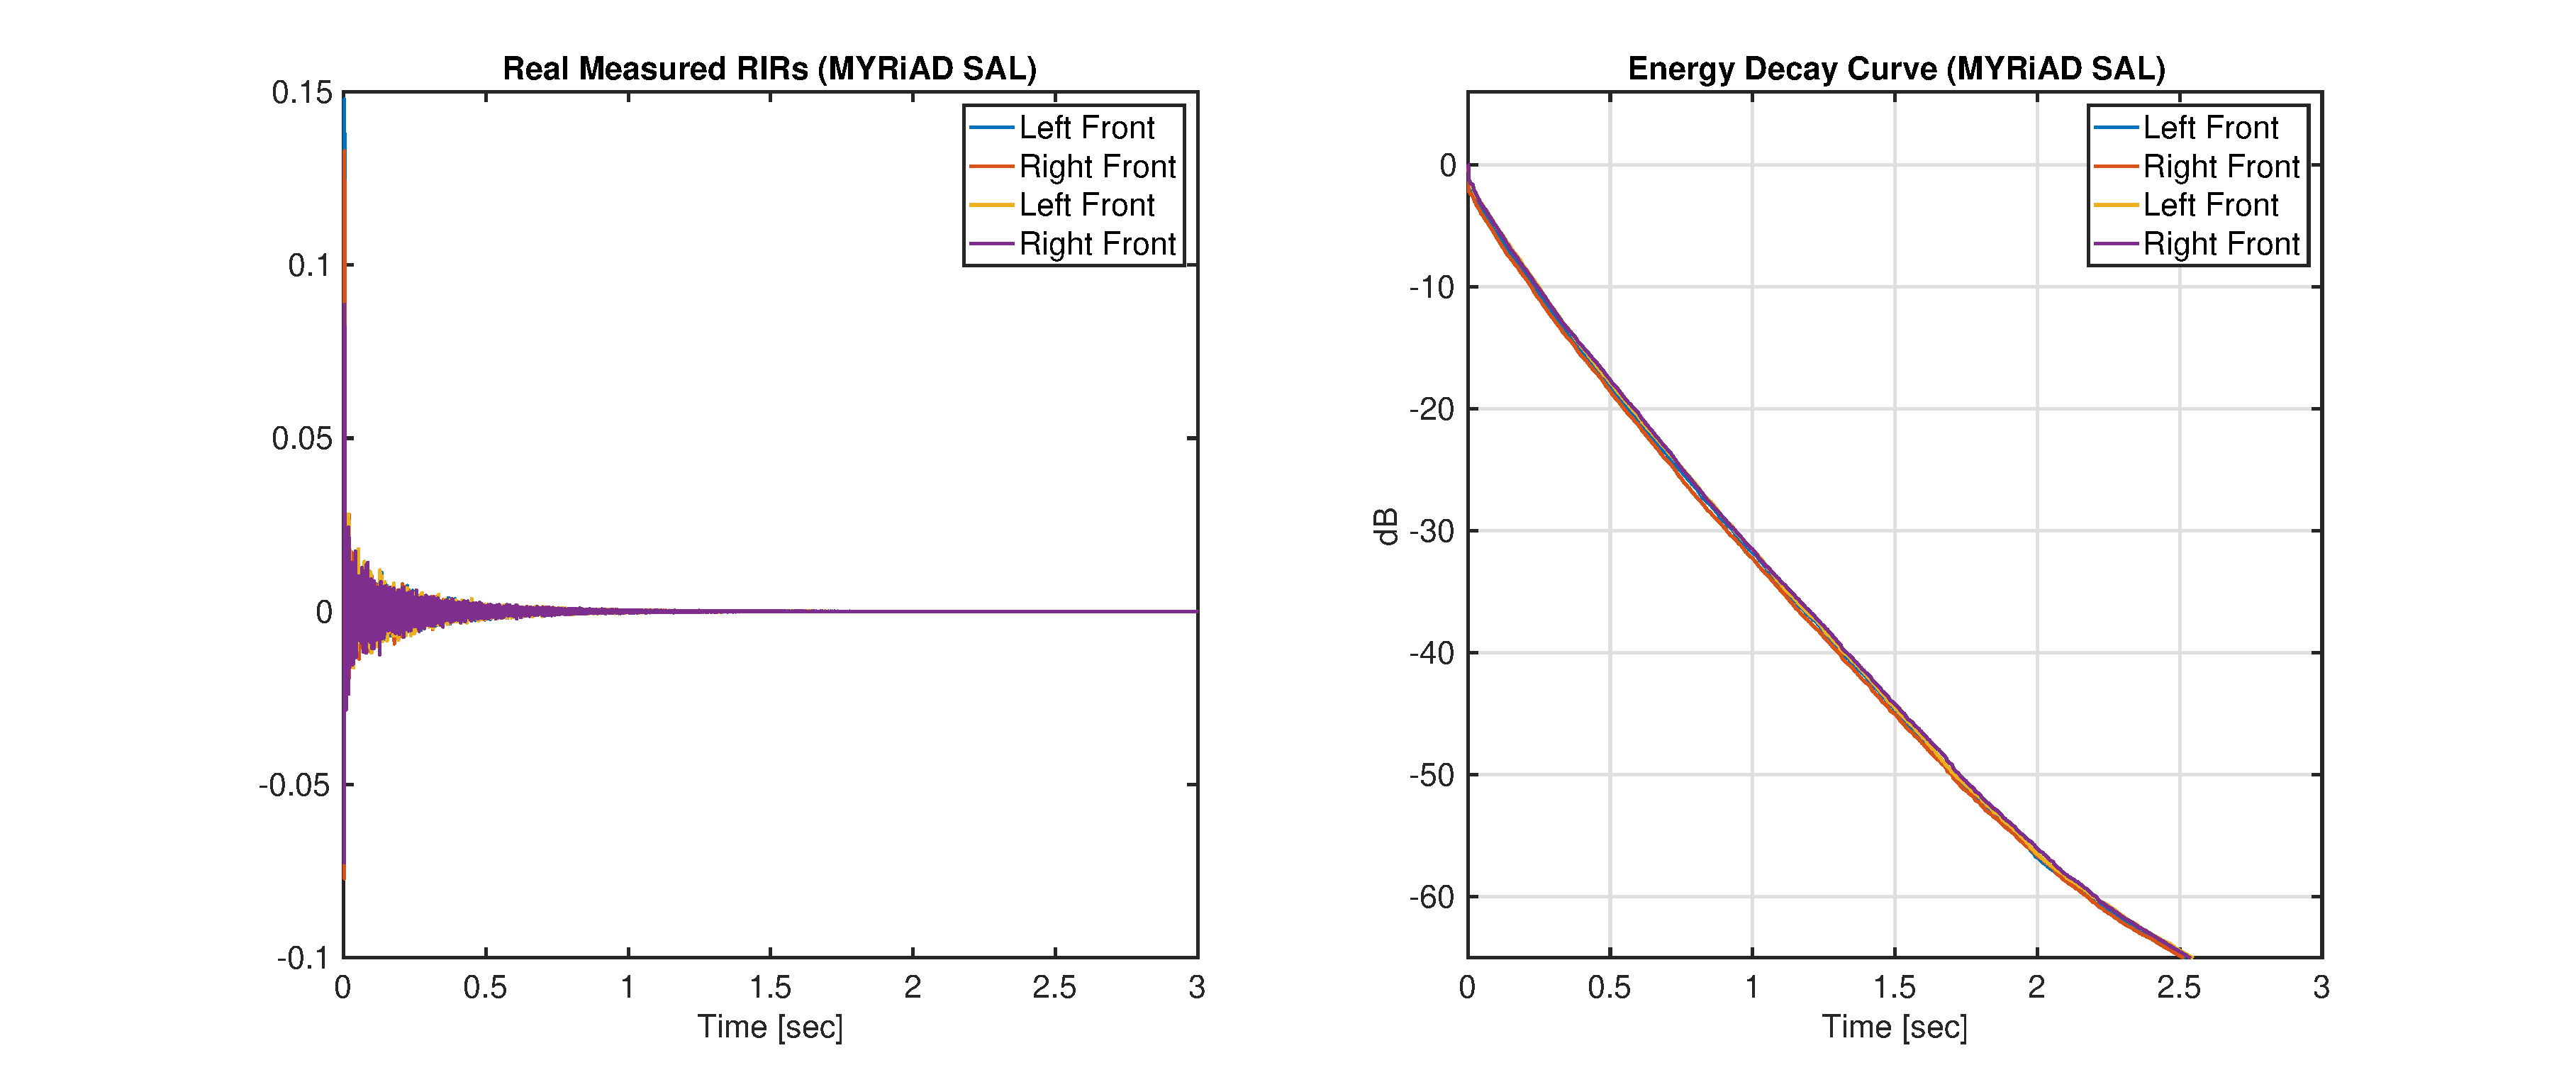
\includegraphics[width=1\textwidth]{RIR_EDC_SAL}
	\centering
	\caption{MYRiAD database SAL room}
	\label{fig:RIR_EDC_SAL}
\end{figure}

•	Listed as 2.1 sec (2100 msec) in paper

•	Measured as approx..

o	T60 = 2200 msec

o	T30 = 2*(1159-100) = 2118 msec


Discuss:

- Add early decay time (EDT) to  chapter 1

- How T60s were calculated in the papers compared to true T60s I'm citing

- EDT of each

- Noise data available also in HRIR (and MYRiAD?)

\subsection{Evaluation of Equalization-Cancellation Front-End}

\textbf{SRM}

\begin{figure}[H]
	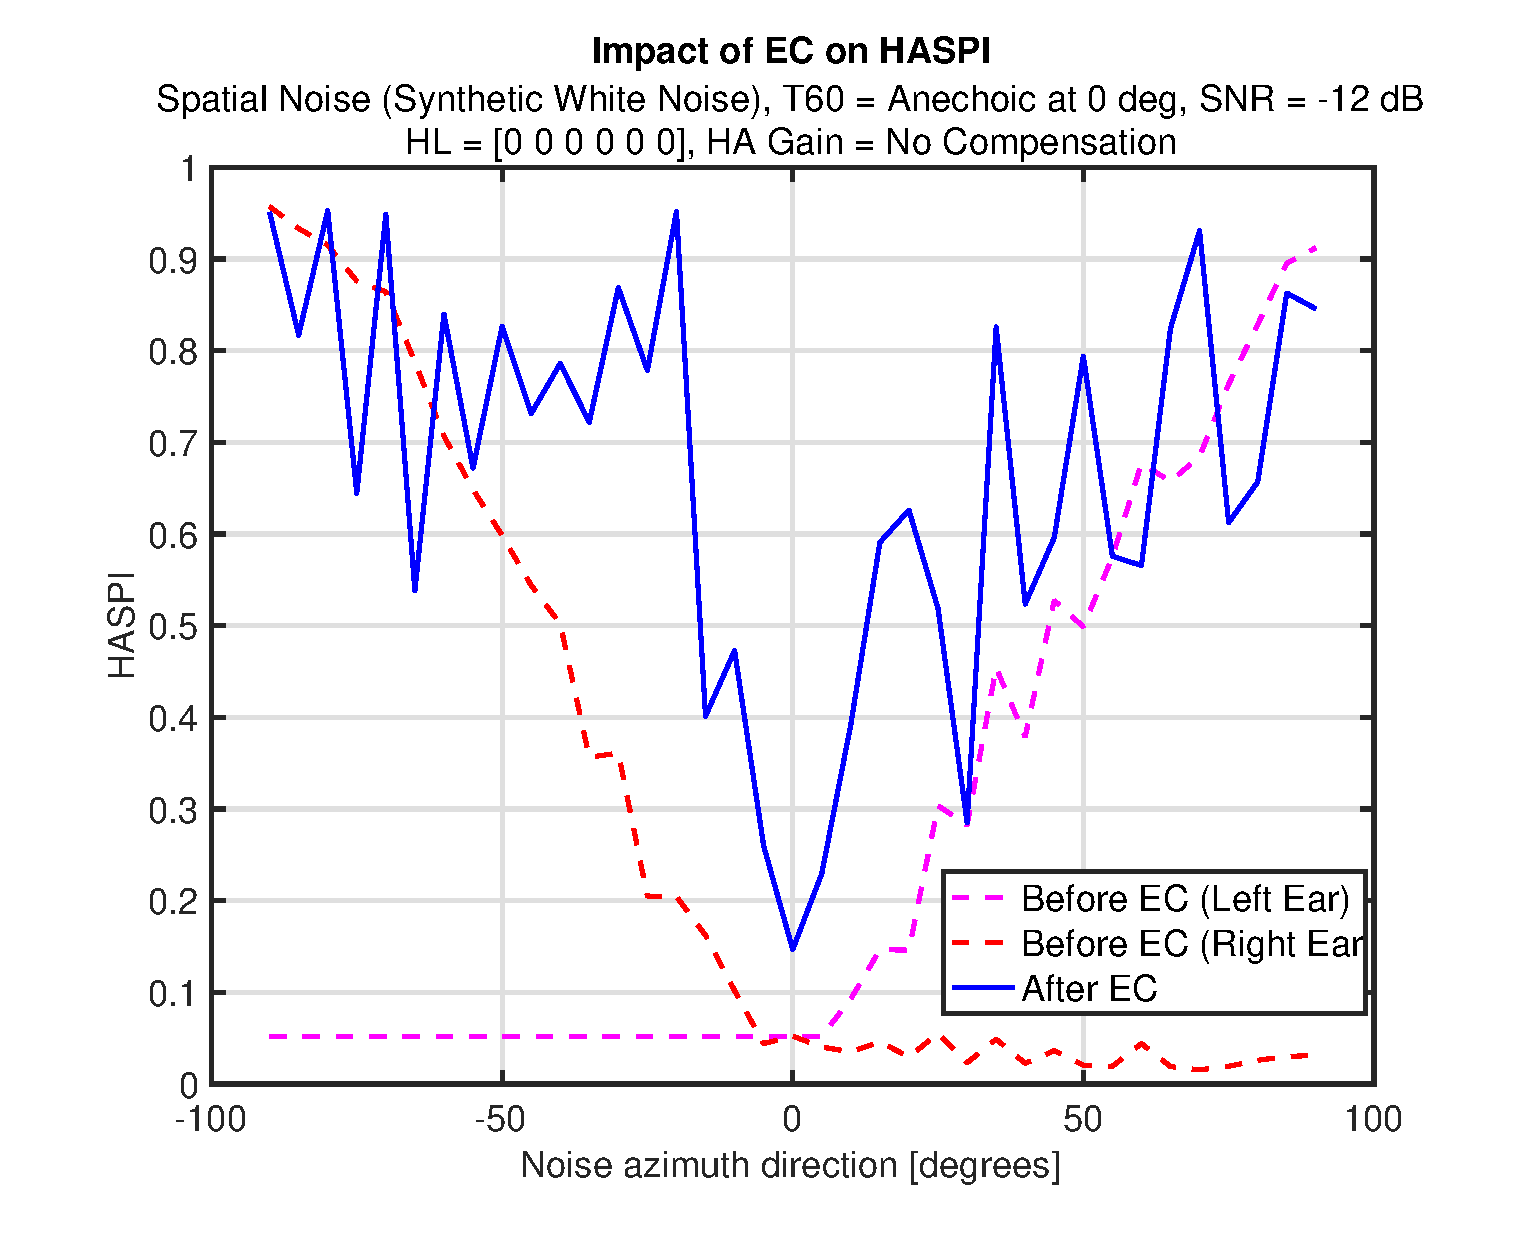
\includegraphics[width=0.7\textwidth]{EC_SRM_NoiseDir}
	\centering
	\caption{Impact of EC algorithm on speech intelligibility (using HASPI) as a function of noise direction, anechoic directional speech and noise}
	\label{fig:EC_SRM_NoiseDir}
\end{figure}

\begin{figure}[H]
	\centering
	\begin{subfigure}[b]{0.49\textwidth}
		\centering
		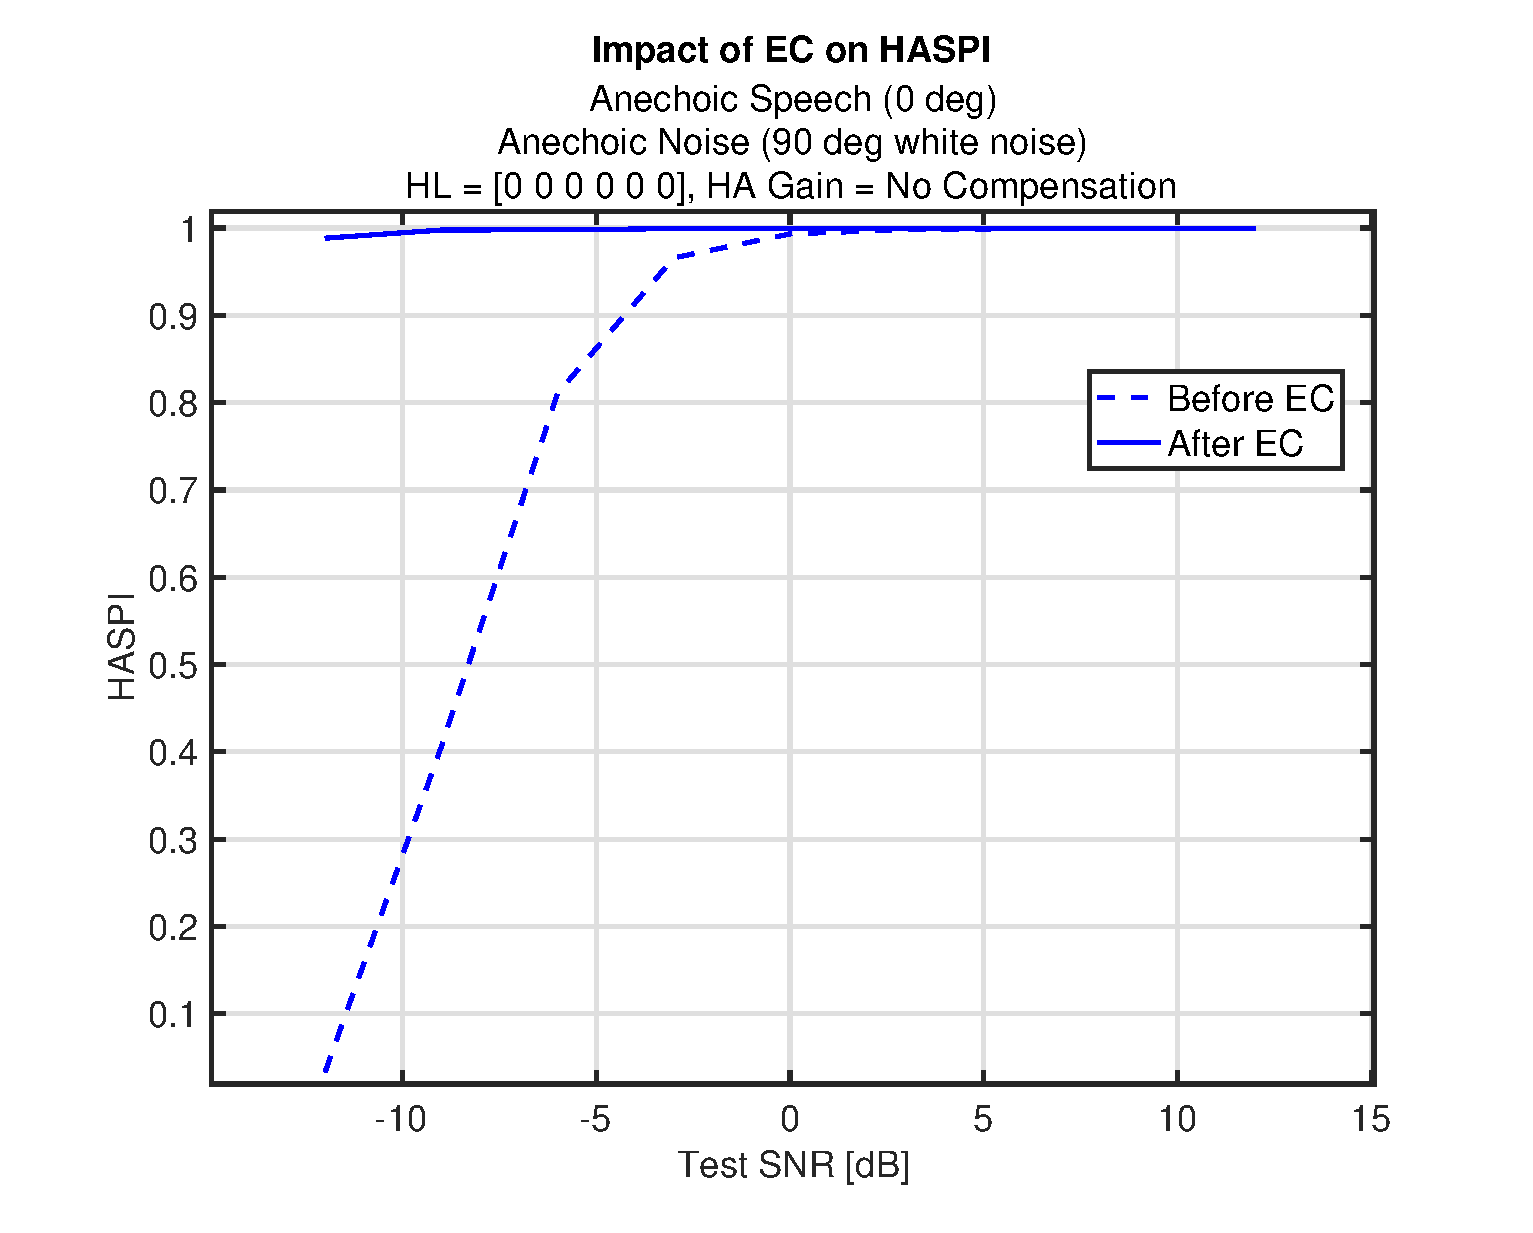
\includegraphics[width=\textwidth]{EC_SRM_AnechoicSpeech_AnechoicNoise}
	\end{subfigure}
	\hfill
	\begin{subfigure}[b]{0.49\textwidth}
		\centering
		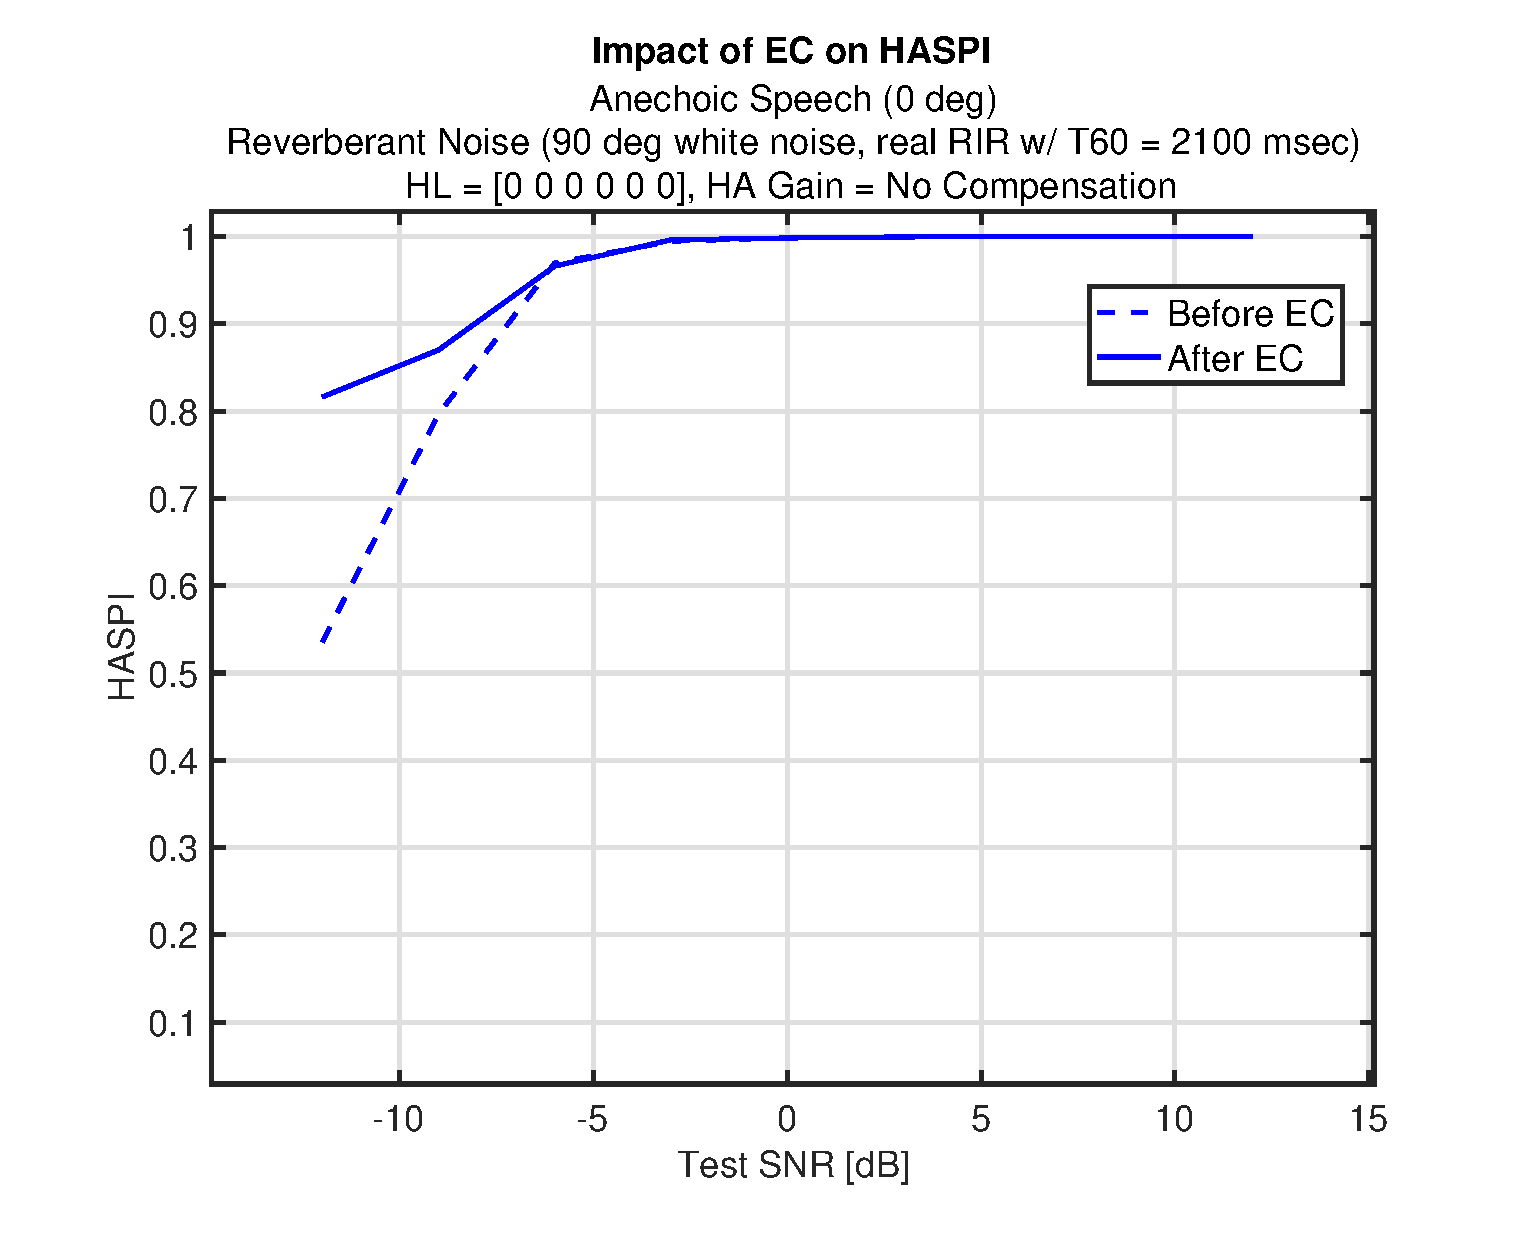
\includegraphics[width=\textwidth]{EC_SRM_AnechoicSpeech_ReverbNoise}
	\end{subfigure}
	\hfill
	\begin{subfigure}[b]{0.49\textwidth}
		\centering
		\includegraphics[width=\textwidth]{EC_SRM_AnechoicSpeech_SpatialNoiseRecording}
	\end{subfigure}
	\hfill
	\begin{subfigure}[b]{0.49\textwidth}
		\centering
		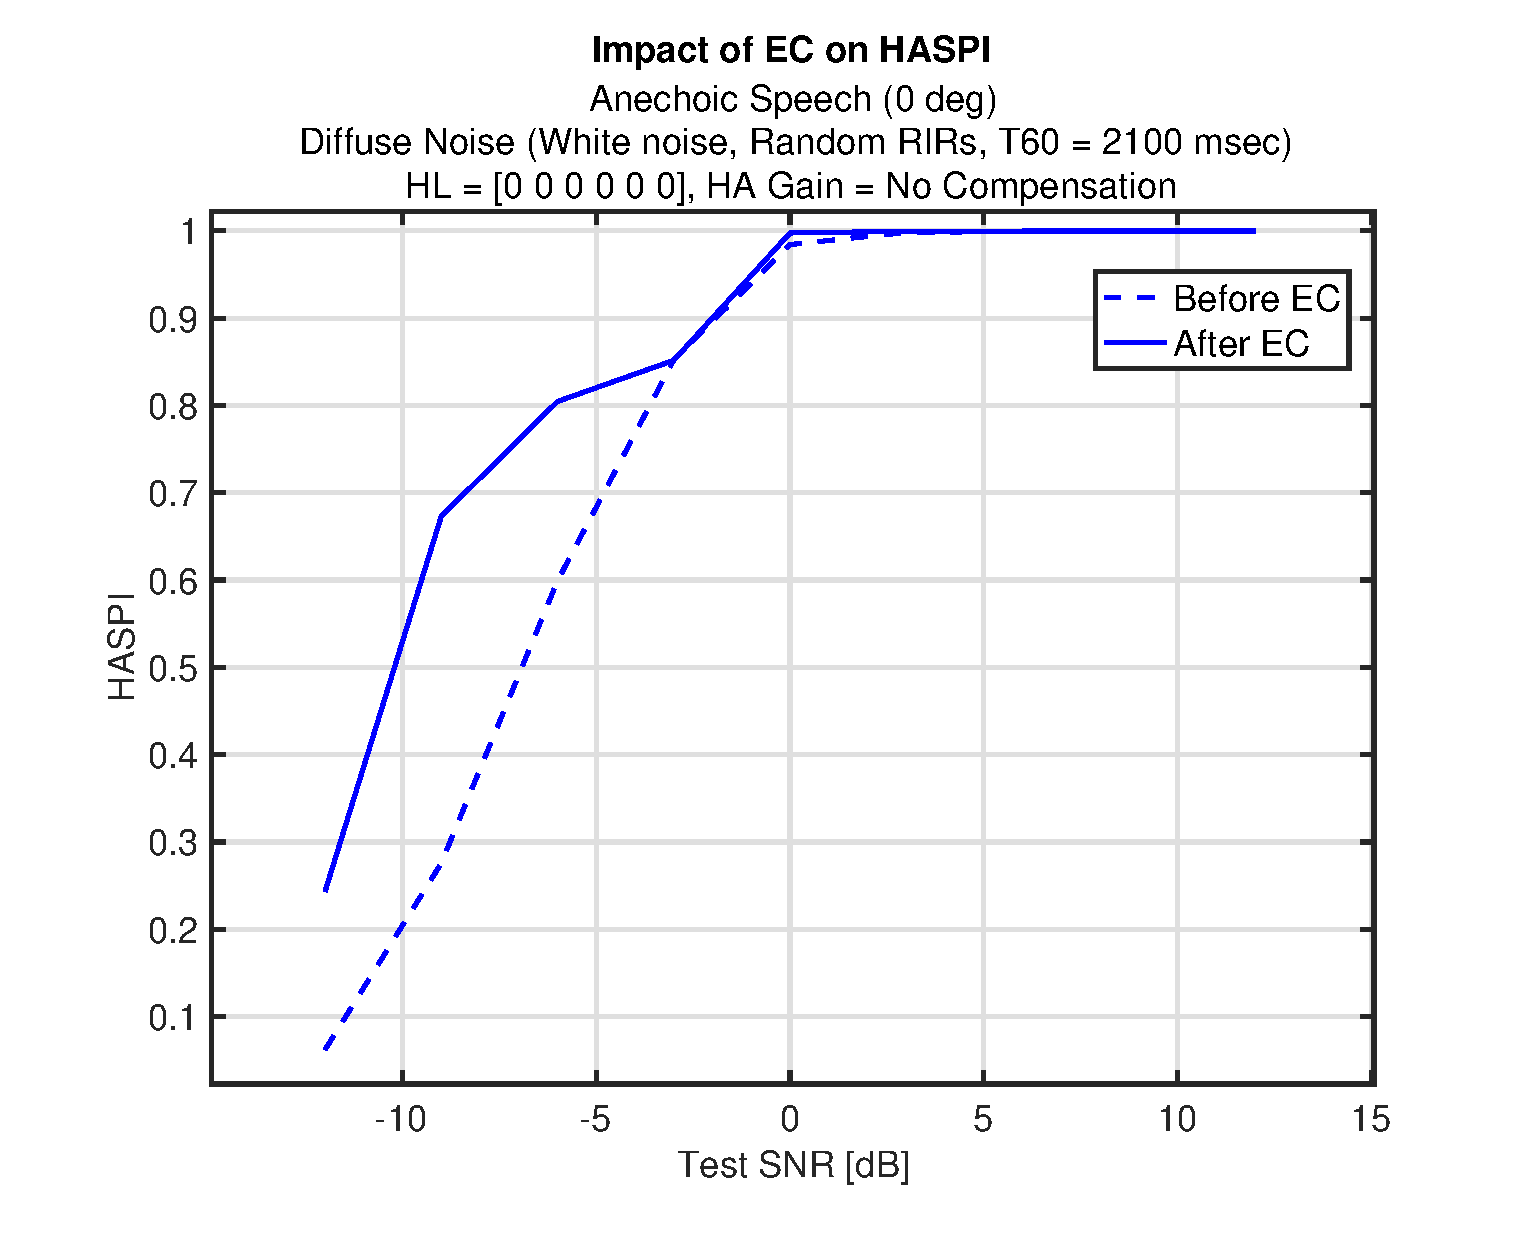
\includegraphics[width=\textwidth]{EC_SRM_AnechoicSpeech_DiffuseNoise}
	\end{subfigure}
	\hfill
	\caption{Impact of EC algorithm on speech intelligibility (using HASPI) as a function of SNR, for anechoic directional speech and various noise types (anechoic directional, reverberant, spatial recording, diffuse)}
	\label{fig:EC_SRM_AnechoicSpeech}
\end{figure}


\begin{figure}[H]
	\centering
	\begin{subfigure}[b]{0.49\textwidth}
		\centering
		\includegraphics[width=\textwidth]{EC_SRM_ReverbSpeech_AnechoicNoise}
	\end{subfigure}
	\hfill
	\begin{subfigure}[b]{0.49\textwidth}
		\centering
		\includegraphics[width=\textwidth]{EC_SRM_ReverbSpeech_ReverbNoise}
	\end{subfigure}
	\hfill
	\begin{subfigure}[b]{0.49\textwidth}
		\centering
		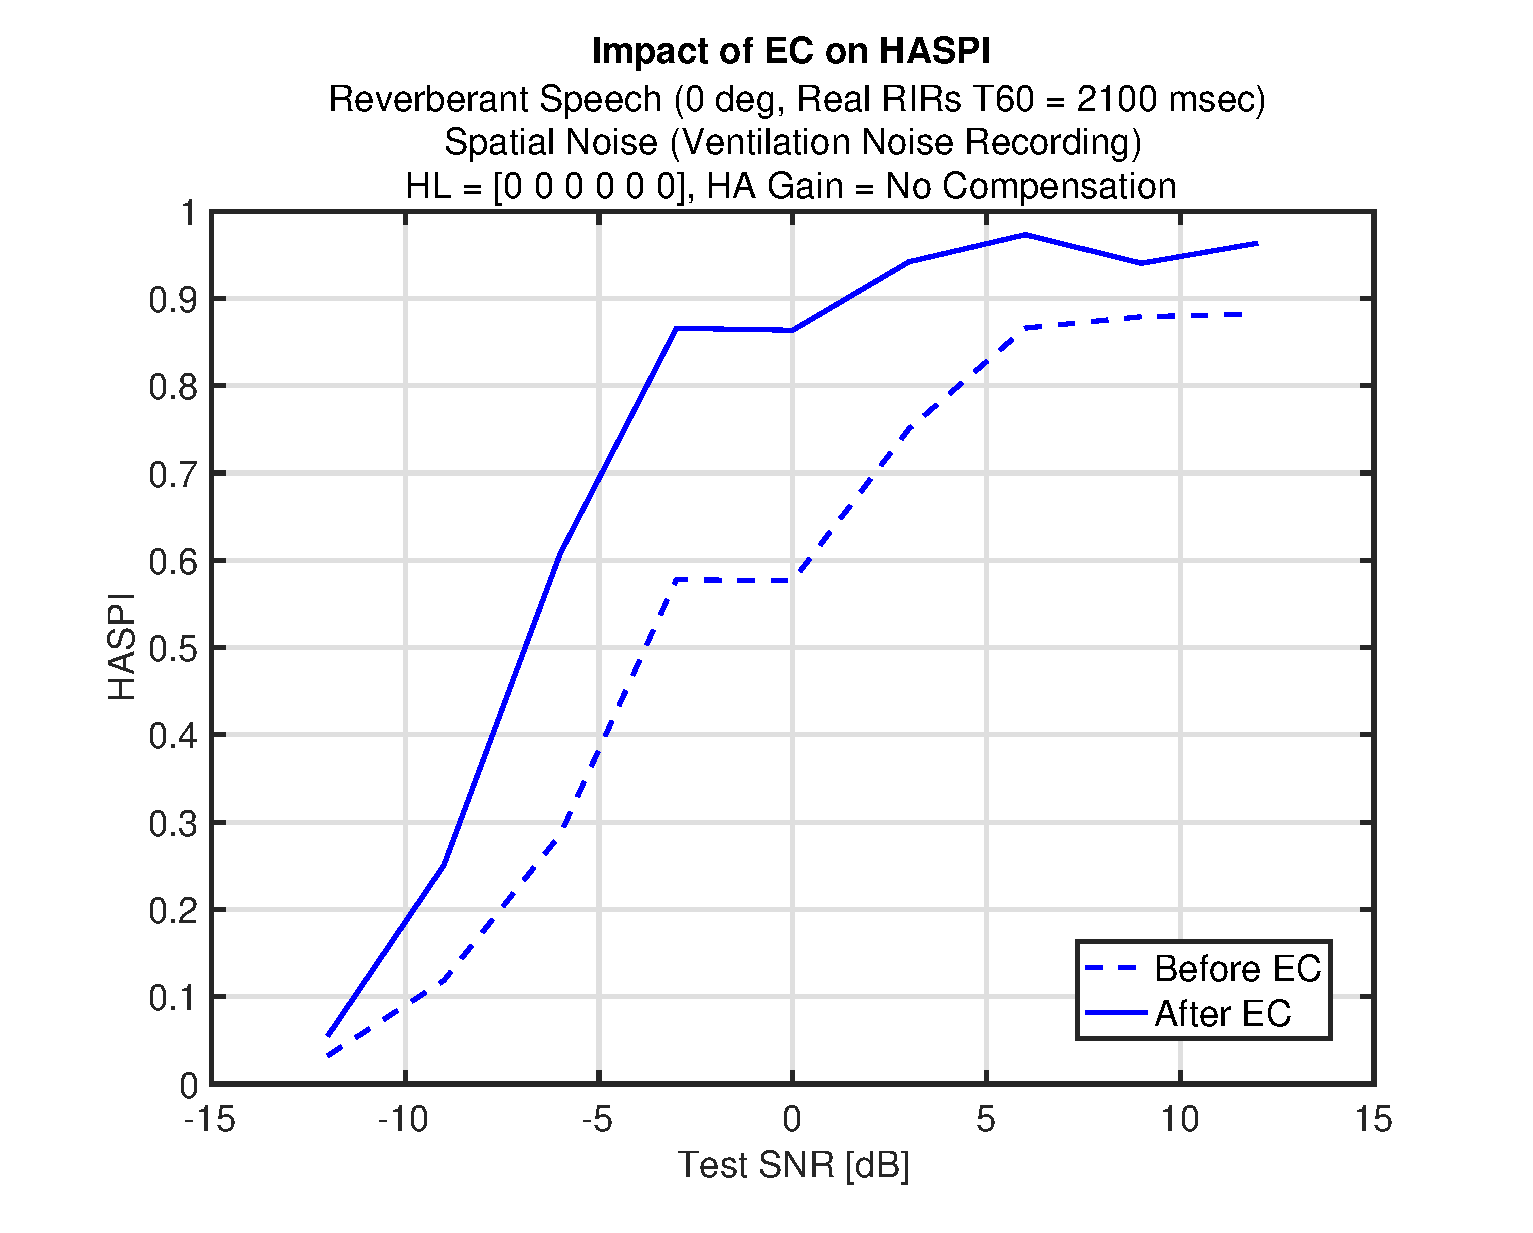
\includegraphics[width=\textwidth]{EC_SRM_ReverbSpeech_SpatialNoiseRecording}
	\end{subfigure}
	\hfill
	\begin{subfigure}[b]{0.49\textwidth}
		\centering
		\includegraphics[width=\textwidth]{EC_SRM_ReverbSpeech_DiffuseNoise}
	\end{subfigure}
	\hfill
	\caption{Impact of EC algorithm on speech intelligibility (using HASPI) as a function of SNR, for reverberant speech and various noise types (anechoic directional, reverberant, spatial recording, diffuse)}
	\label{fig:EC_SRM_ReverbSpeech}
\end{figure}


\begin{figure}[H]
	\centering
	\begin{subfigure}[b]{0.49\textwidth}
		\centering
		\includegraphics[width=\textwidth]{EC_SRM_DiffuseSpeech_AnechoicNoise}
	\end{subfigure}
	\hfill
	\begin{subfigure}[b]{0.49\textwidth}
		\centering
		\includegraphics[width=\textwidth]{EC_SRM_DiffuseSpeech_ReverbNoise}
	\end{subfigure}
	\hfill
	\begin{subfigure}[b]{0.49\textwidth}
		\centering
		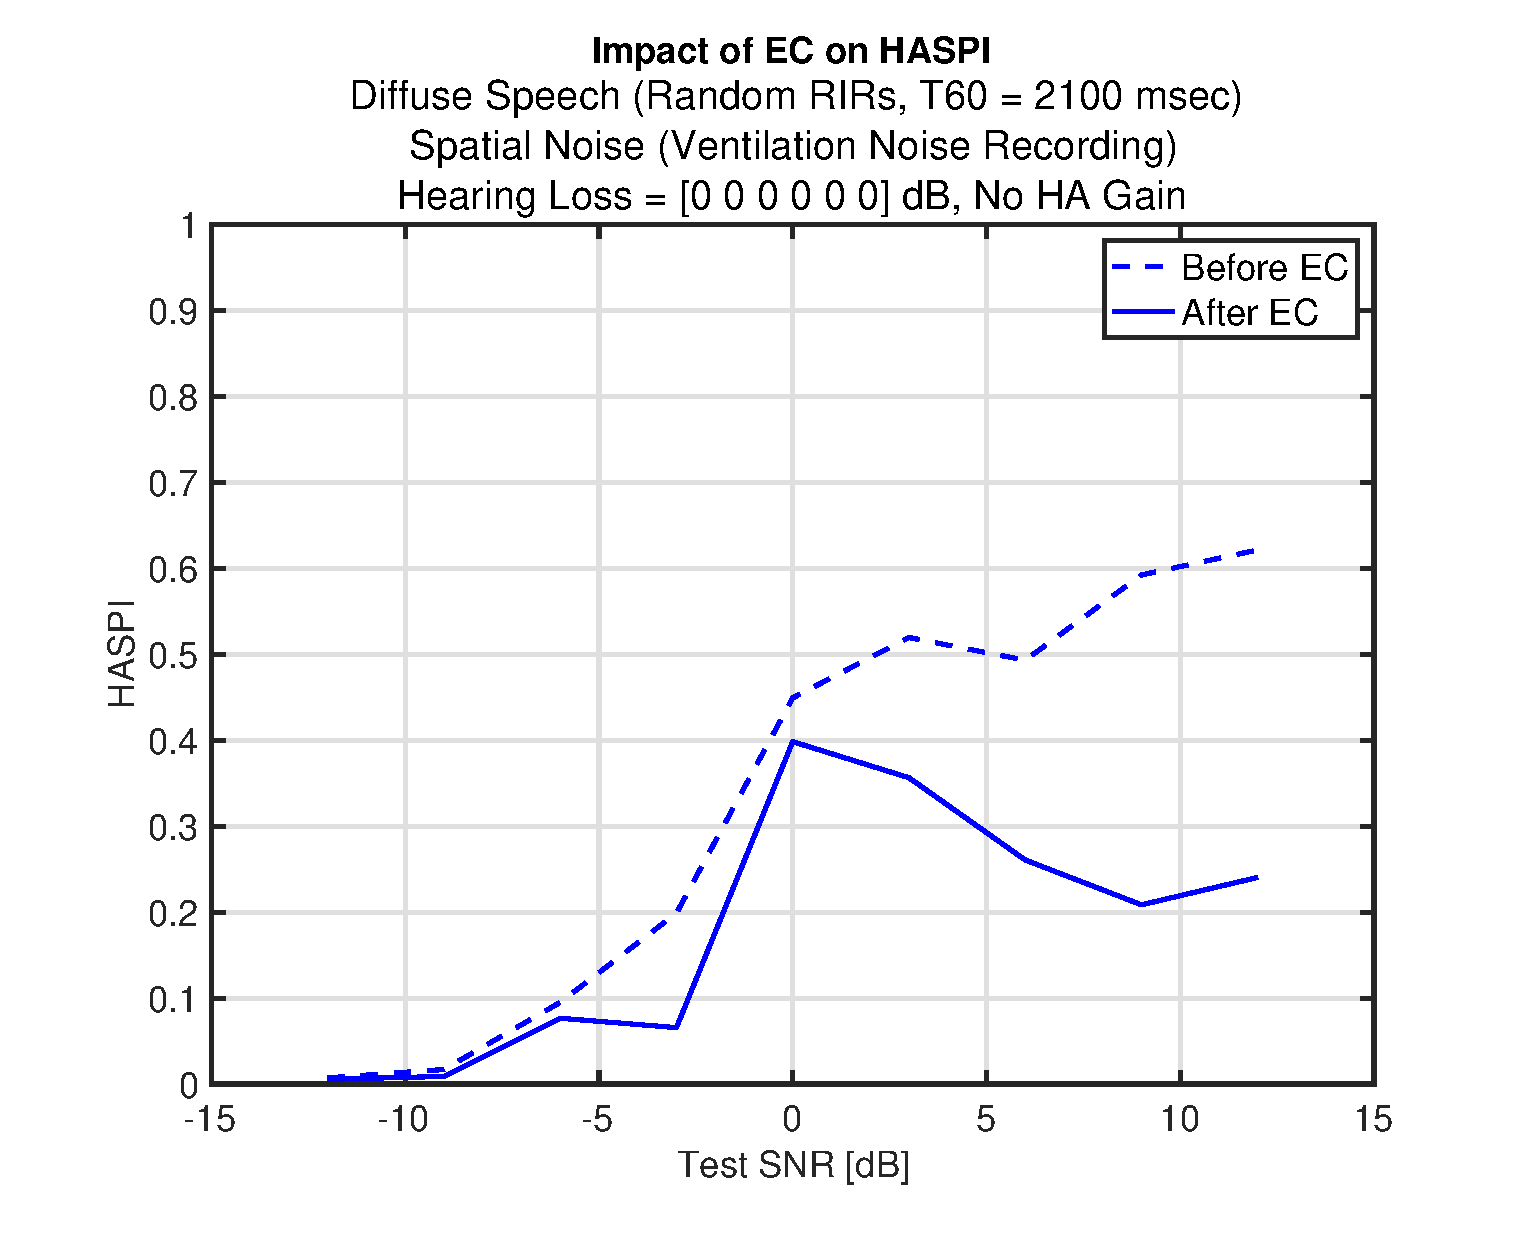
\includegraphics[width=\textwidth]{EC_SRM_DiffuseSpeech_SpatialNoiseRecording}
	\end{subfigure}
	\hfill
	\begin{subfigure}[b]{0.49\textwidth}
		\centering
		\includegraphics[width=\textwidth]{EC_SRM_DiffuseSpeech_DiffuseNoise}
	\end{subfigure}
	\hfill
	\caption{Impact of EC algorithm on speech intelligibility (using HASPI) as a function of SNR, for diffuse speech and various noise types (anechoic directional, reverberant, spatial recording, diffuse)}
	\label{fig:EC_SRM_DiffuseSpeech}
\end{figure}


\textbf{Impact of reverb on binaural benefit modeled by EC}


\begin{figure}[H]
	\centering
	\begin{subfigure}[b]{0.49\textwidth}
		\centering
		\includegraphics[width=\textwidth]{EC_SRM_T60_SNRm12}
	\end{subfigure}
	\hfill
	\begin{subfigure}[b]{0.49\textwidth}
		\centering
		\includegraphics[width=\textwidth]{EC_SRM_T60_SNR0}
	\end{subfigure}
	\caption{Impact of EC algorithm on speech intelligibility (using HASPI) as a function of varying amounts of synthetic reverb, for spatial noise recording with SNR = \qty{-12}{\decibel} and SNR = \qty{0}{\decibel}}
	\label{fig:EC_SRM_T60}
\end{figure}

- Diffuse reverb destroys binaural cues and reduces the binaural benefit modeled by the EC (this provides modeling of the reduction in SRM due to reverb). However at low T60s the RIR is less diffuse and therefore can randomly have more emphasized directions thus sometimes providing some binaural benefit
- Note distinction between SRM for noise and reverb (EC models reduction in SRM due to reverb, but doesnt model reduction in reverb itself)

- SNR = 0 dB: SI is already saturated, so only evaluating impact of reverb (essentially SNR = infinity)

\textbf{Does EC capture any of the benefits of early reflections?}


\begin{figure}[H]
	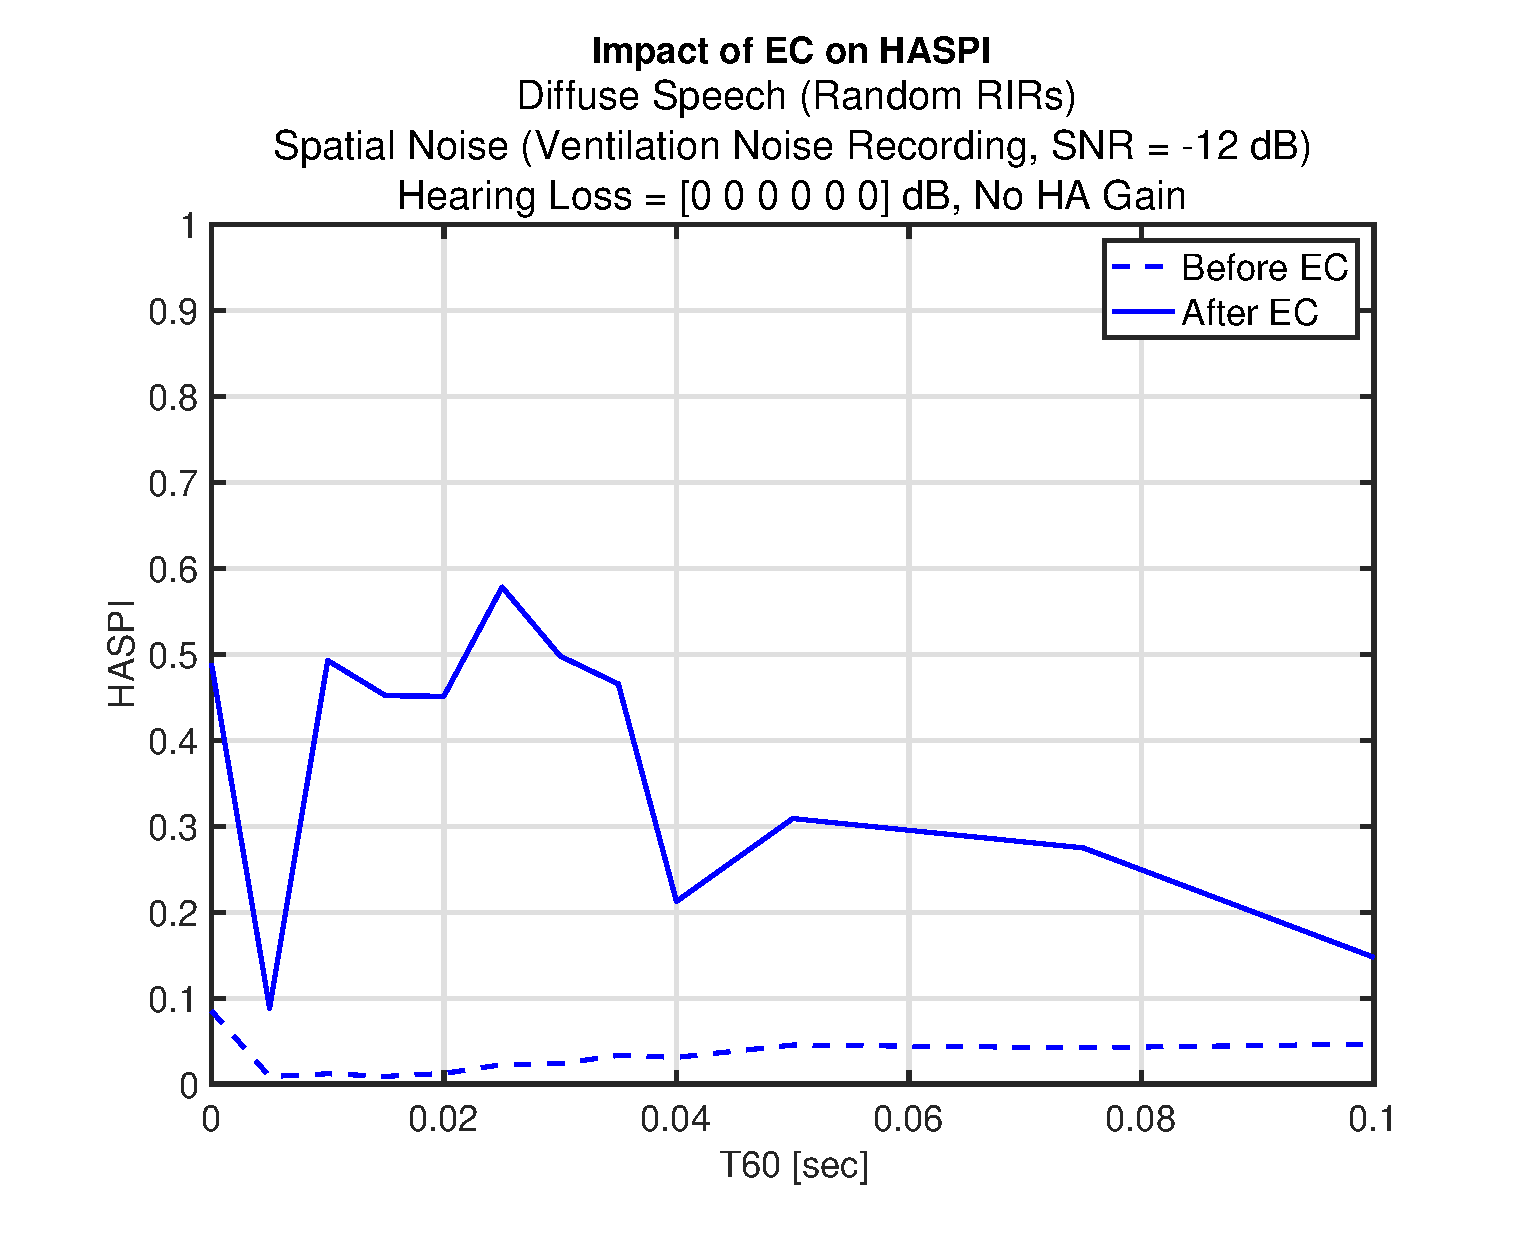
\includegraphics[width=0.7\textwidth]{EC_ERs}
	\centering
	\caption{Impact of EC algorithm on speech intelligibility (using HASPI) as a function of varying amounts of synthetic reverb, for spatial noise recording with SNR = \qty{-12}{\decibel}  }
	\label{fig:EC_ReverbSNRBoost}
\end{figure}

- Diffuse reverb (white noise) used to focus on temporal integration rather than spatial separation -- Most significant binaural benefit for T60 = 0 (no benefit of early reflections) -- However repeating the experiment several times reveals occasional benefit depending on the randomly generated RIR -- assumed this is just due to sometimese the very short number of simulated reflections effectively coming from similar directions thus providing SRM

- I would expect that using real RIRs would result in some SRM from early reflections (since they tend not to be diffuse)

- Essentially all this shows that EC may provide some modeling of BINAURAL benefit of reverb in low SNR environments (SRM), but no modeling of MONAURAL benefit of reverb (PE temporal integration)


\textbf{EC on reverb only}

\begin{figure}[H]
	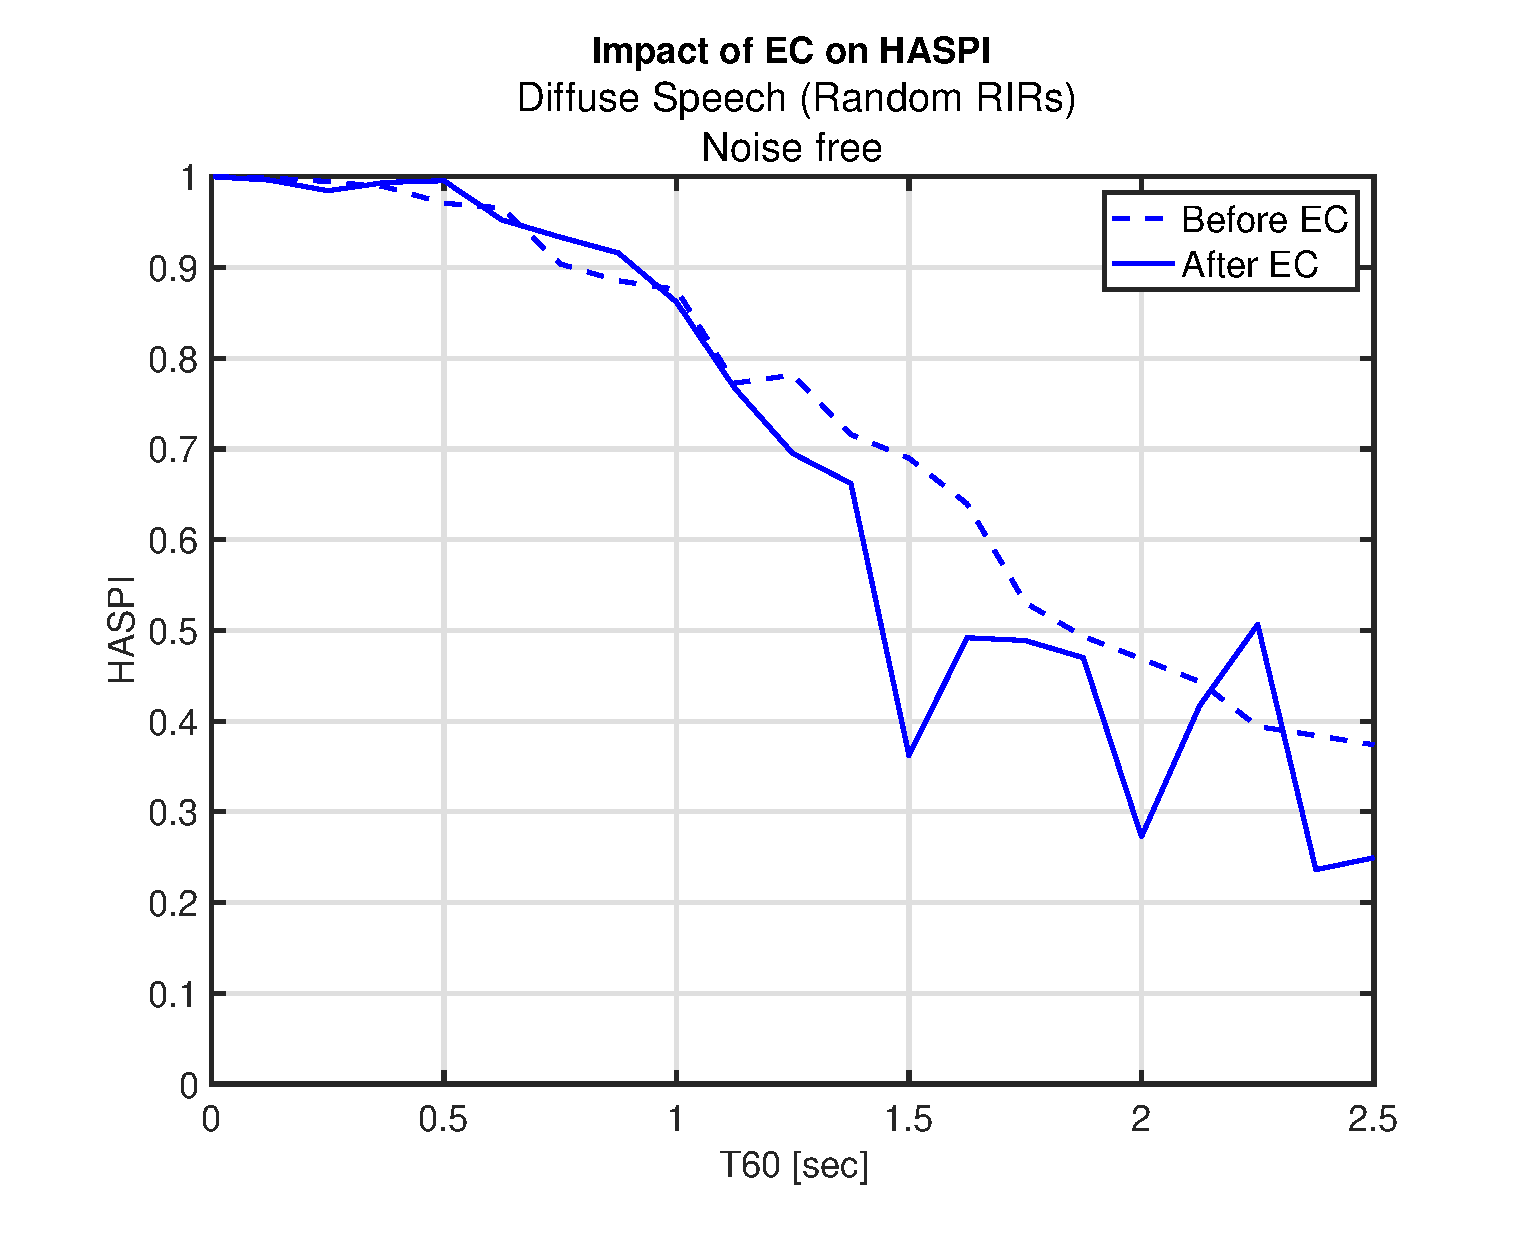
\includegraphics[width=0.7\textwidth]{EC_SRM_T60_SNR300}
	\centering
	\caption{Impact of EC algorithm on speech intelligibility (using HASPI) as a function of varying amounts of synthetic reverb, noise-free}
	\label{fig:EC_SRM_T60_SNR300}
\end{figure}

- EC does not provide binaural benefit in reverb

- EC focuses on canceling interfering noise from certain directions, which doesnt apply to reducing reverb since (for high T60s) reverb tends towards diffuse, and the interfering reflections are correlated to the clean speech



\subsection{Hearing Aid Gain Comparison}

Ian:

- Loudness recruitment and its influence on WDRC design (Threshold of hearing increasing doesnt increase in upper limit where loudness becomes too much -- reduced dynamic range)

- Question: Do nonlinearities in auditory system still apply at same higher SPL with hearing loss? If so then this is another reason for not doing mirror audiogram compensation (not just comfort, but going to these high levels will distort cues making SI worse -- Shouldnt this be picked up by the metrics?)

- Look at Hearing Aid textbook from Harvey Dillon

- NAL-R ideal at conversational speech, quieter you want closer to mirror audiogram, and louder sounds you want less than NAL-R

- Generally speaking in terms of restoring the representation (maybe also in STMI/NSIM -- pretty sure Ian knows but im missing something) mirror audiogram will be optimal for SI, NAL-R is more about comfort -- We cant do mirror audiogram because users wont like it, NAL-R is better in terms of trade off of SI and comfort

\begin{figure}[H]
	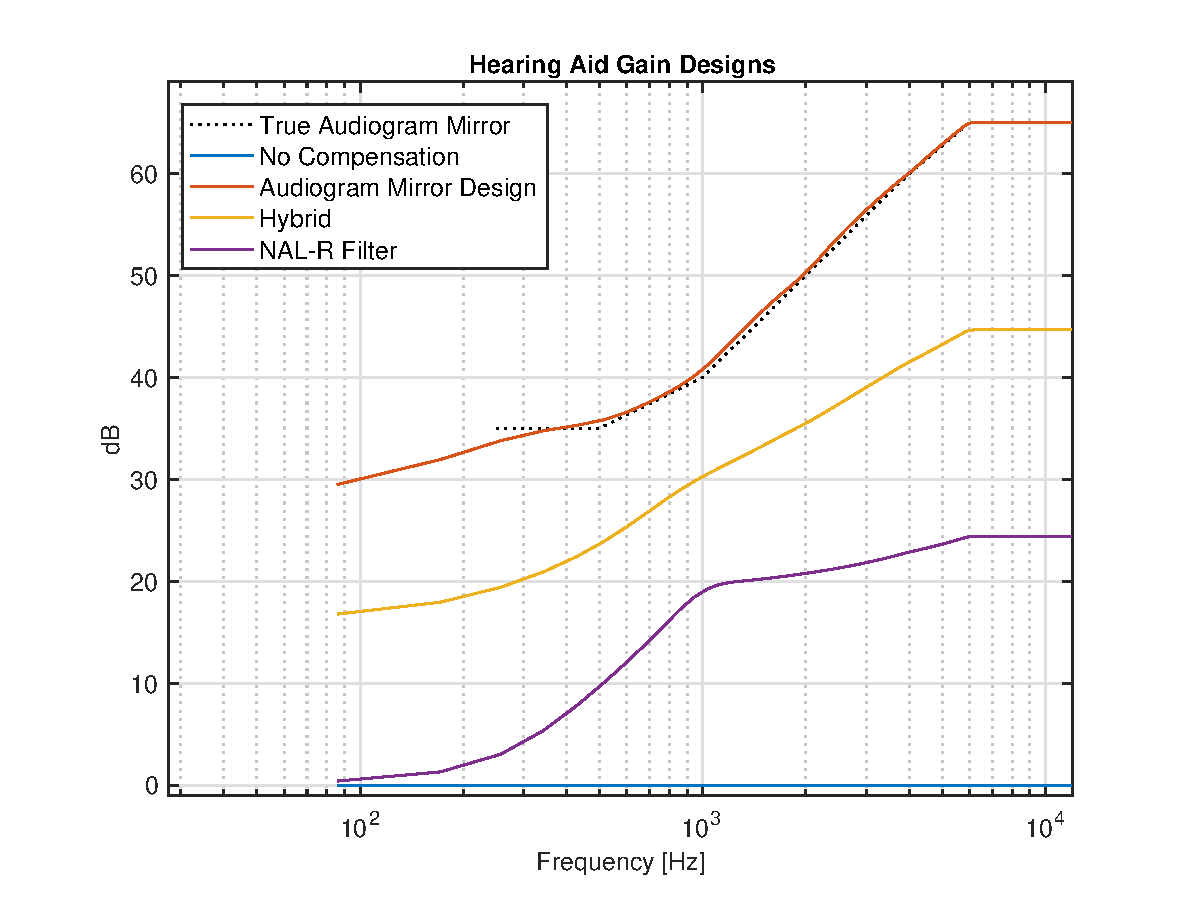
\includegraphics[width=0.7\textwidth]{HearingAidGains}
	\centering
	\caption{Hearing aid gains to be used in evaluation}
	\label{fig:HA_Gains}
\end{figure}

\begin{figure}[H]
	\centering
	\begin{subfigure}[b]{0.49\textwidth}
		\centering
		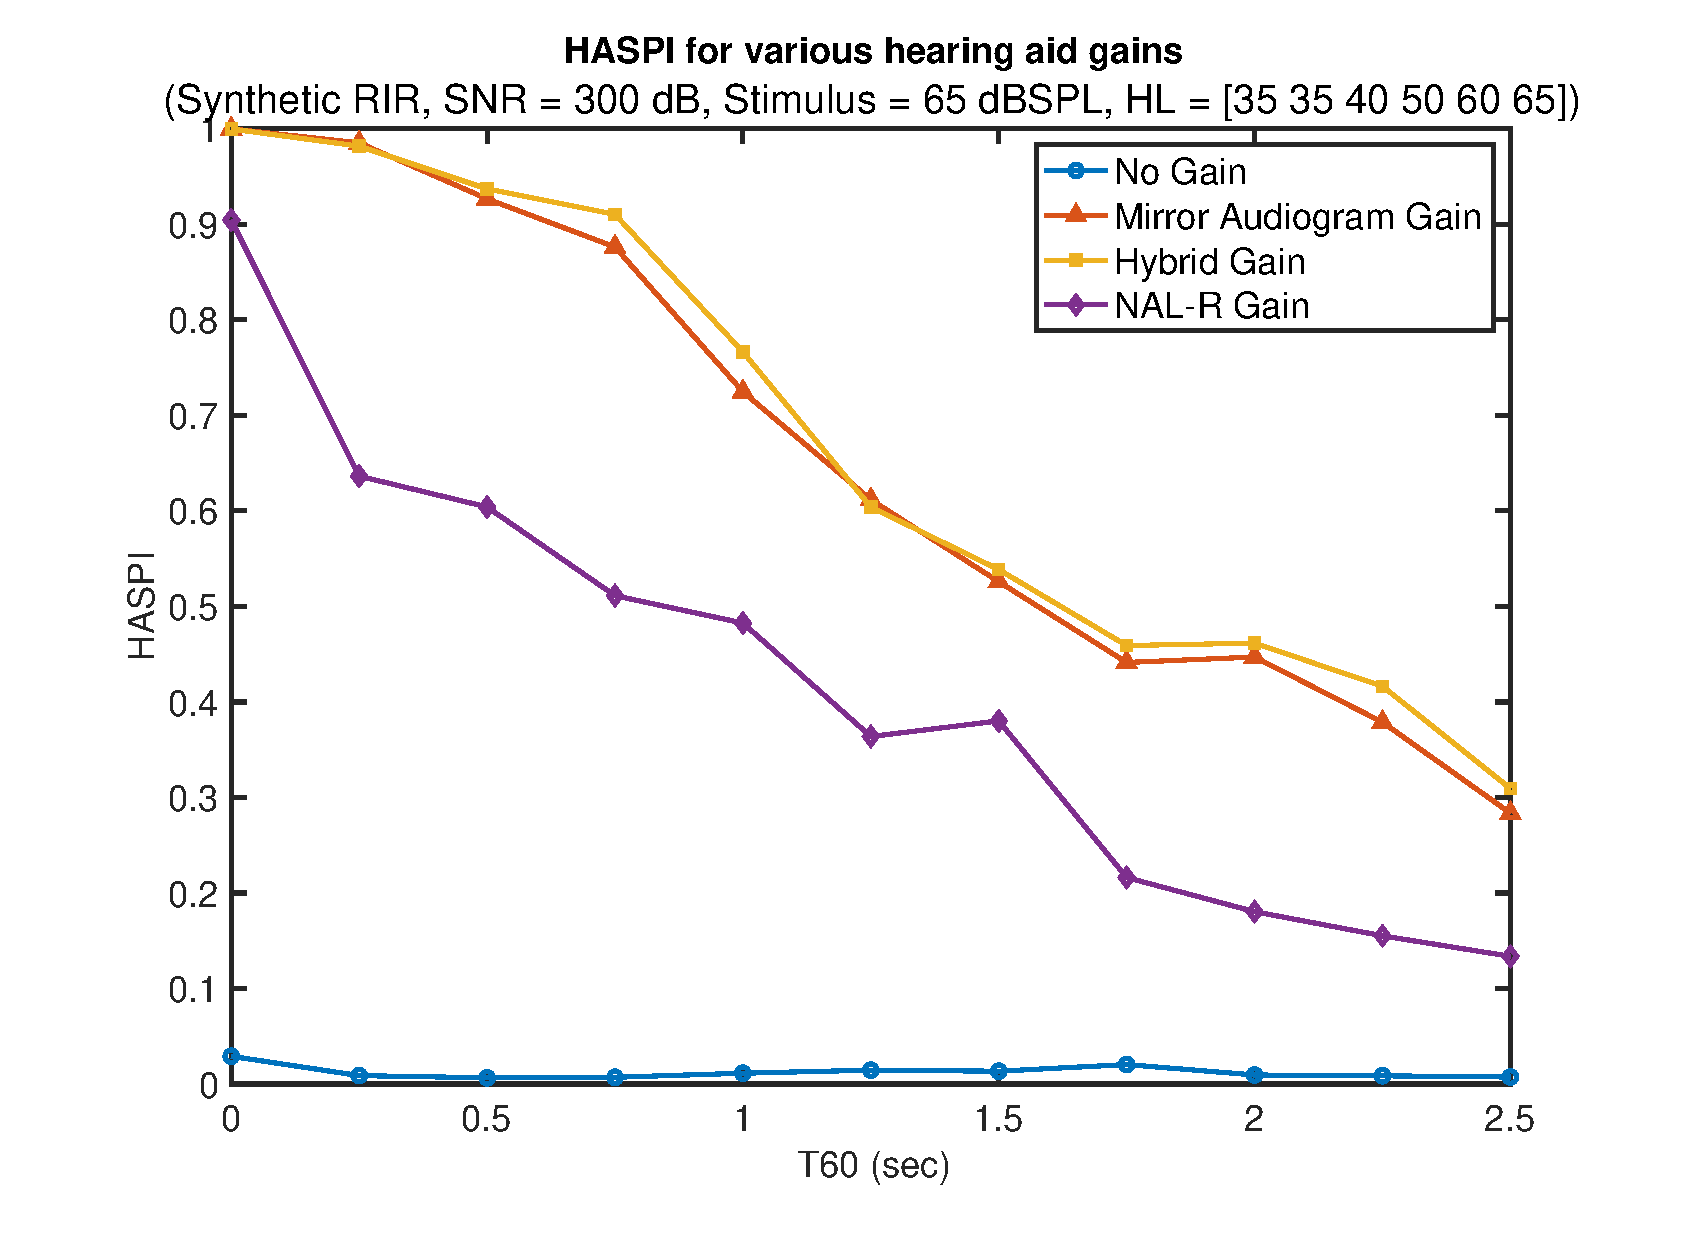
\includegraphics[width=\textwidth]{HASPI_v_T60_variousHAGains}
	\end{subfigure}
	\hfill
	\begin{subfigure}[b]{0.49\textwidth}
		\centering
		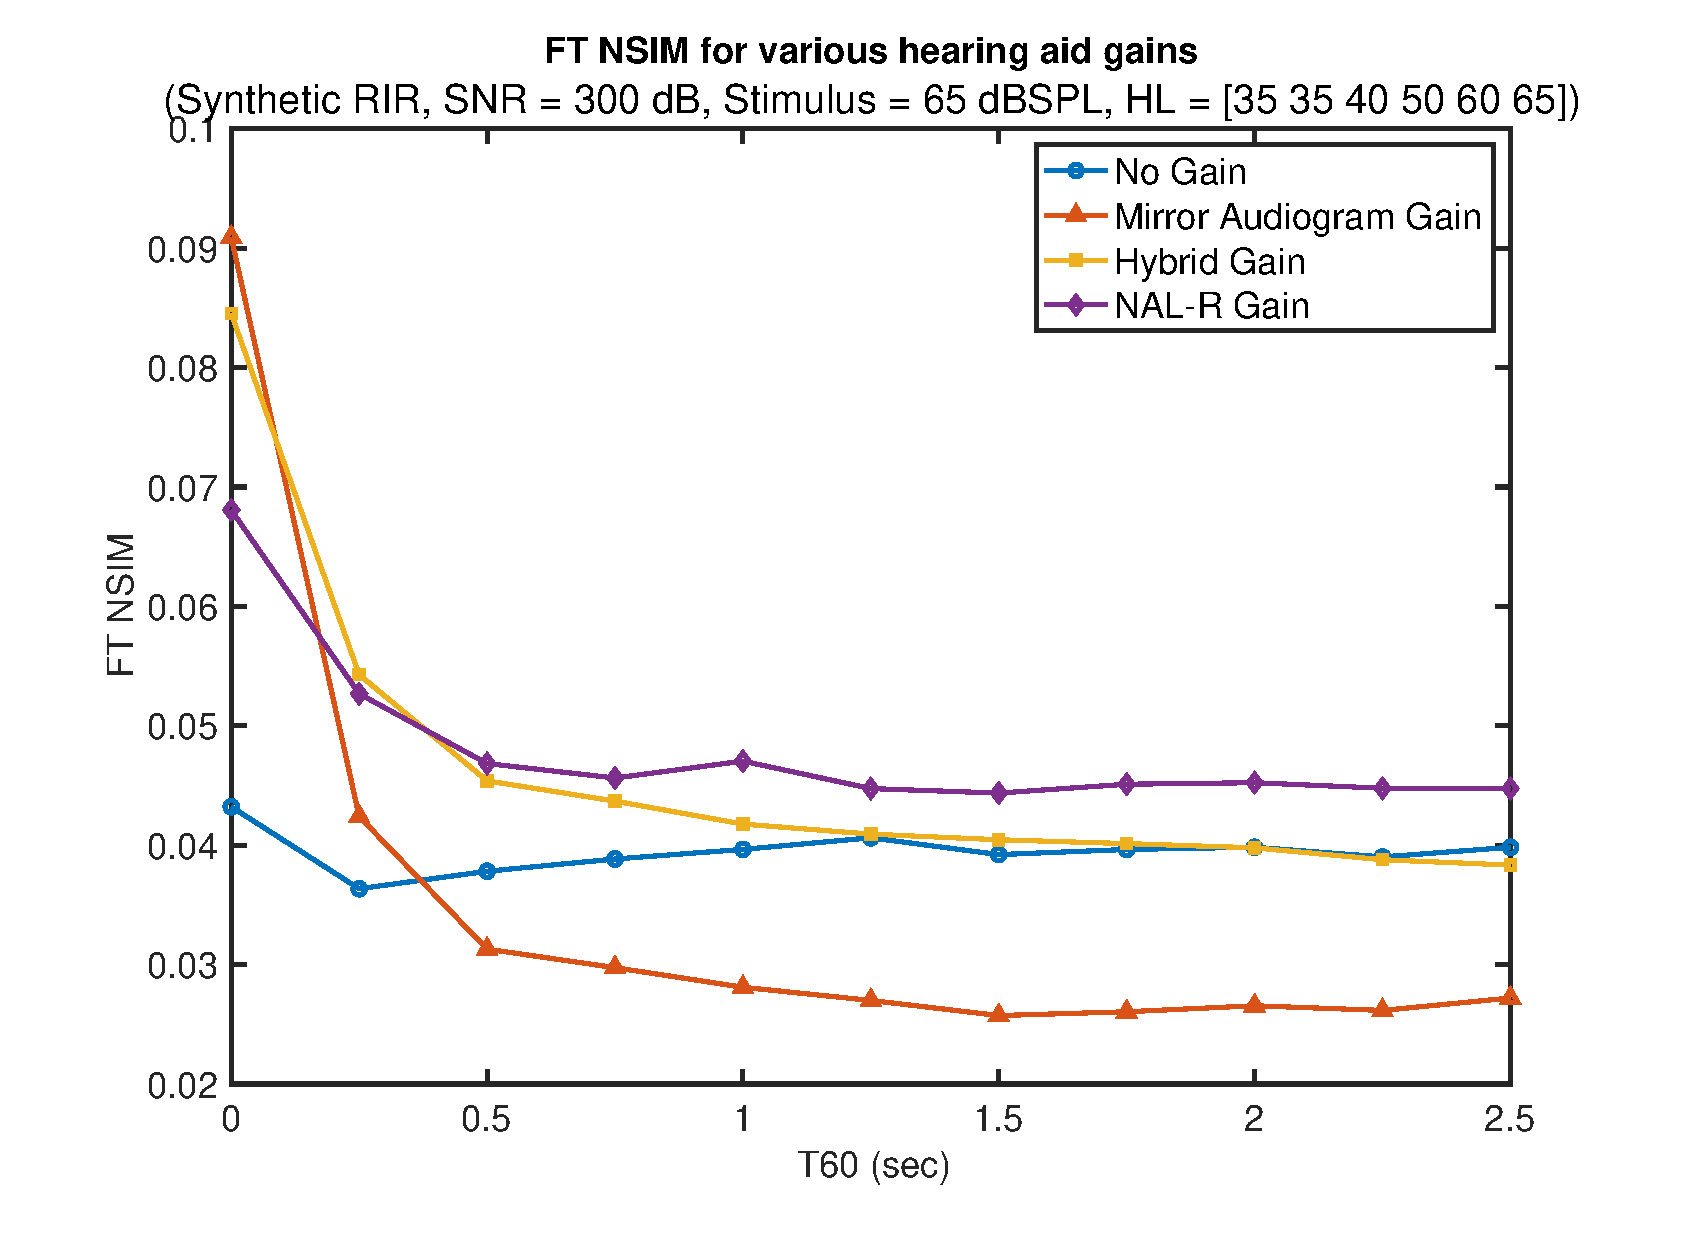
\includegraphics[width=\textwidth]{NSIM_FT_v_T60_variousHAGains}
	\end{subfigure}
	\hfill
	\begin{subfigure}[b]{0.49\textwidth}
		\centering
		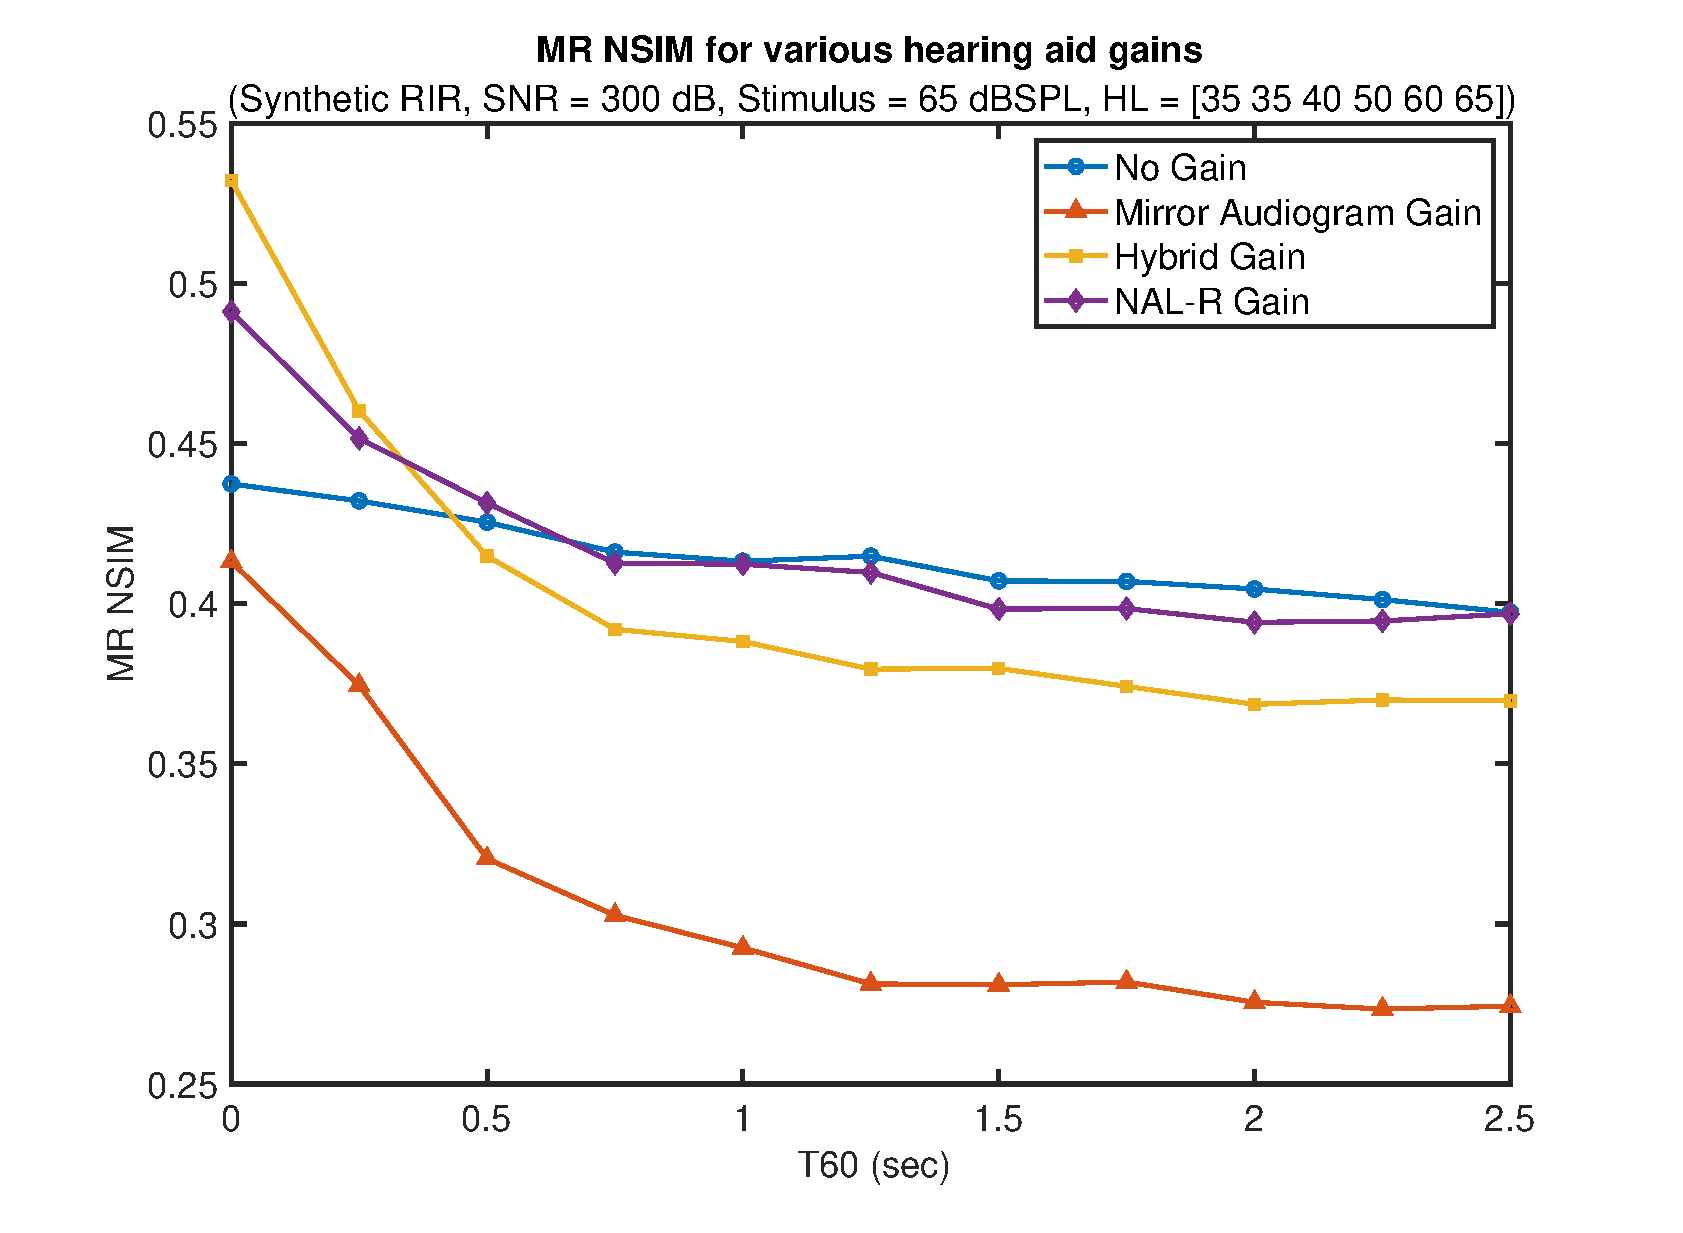
\includegraphics[width=\textwidth]{NSIM_MR_v_T60_variousHAGains}
	\end{subfigure}
	\hfill
	\begin{subfigure}[b]{0.49\textwidth}
		\centering
		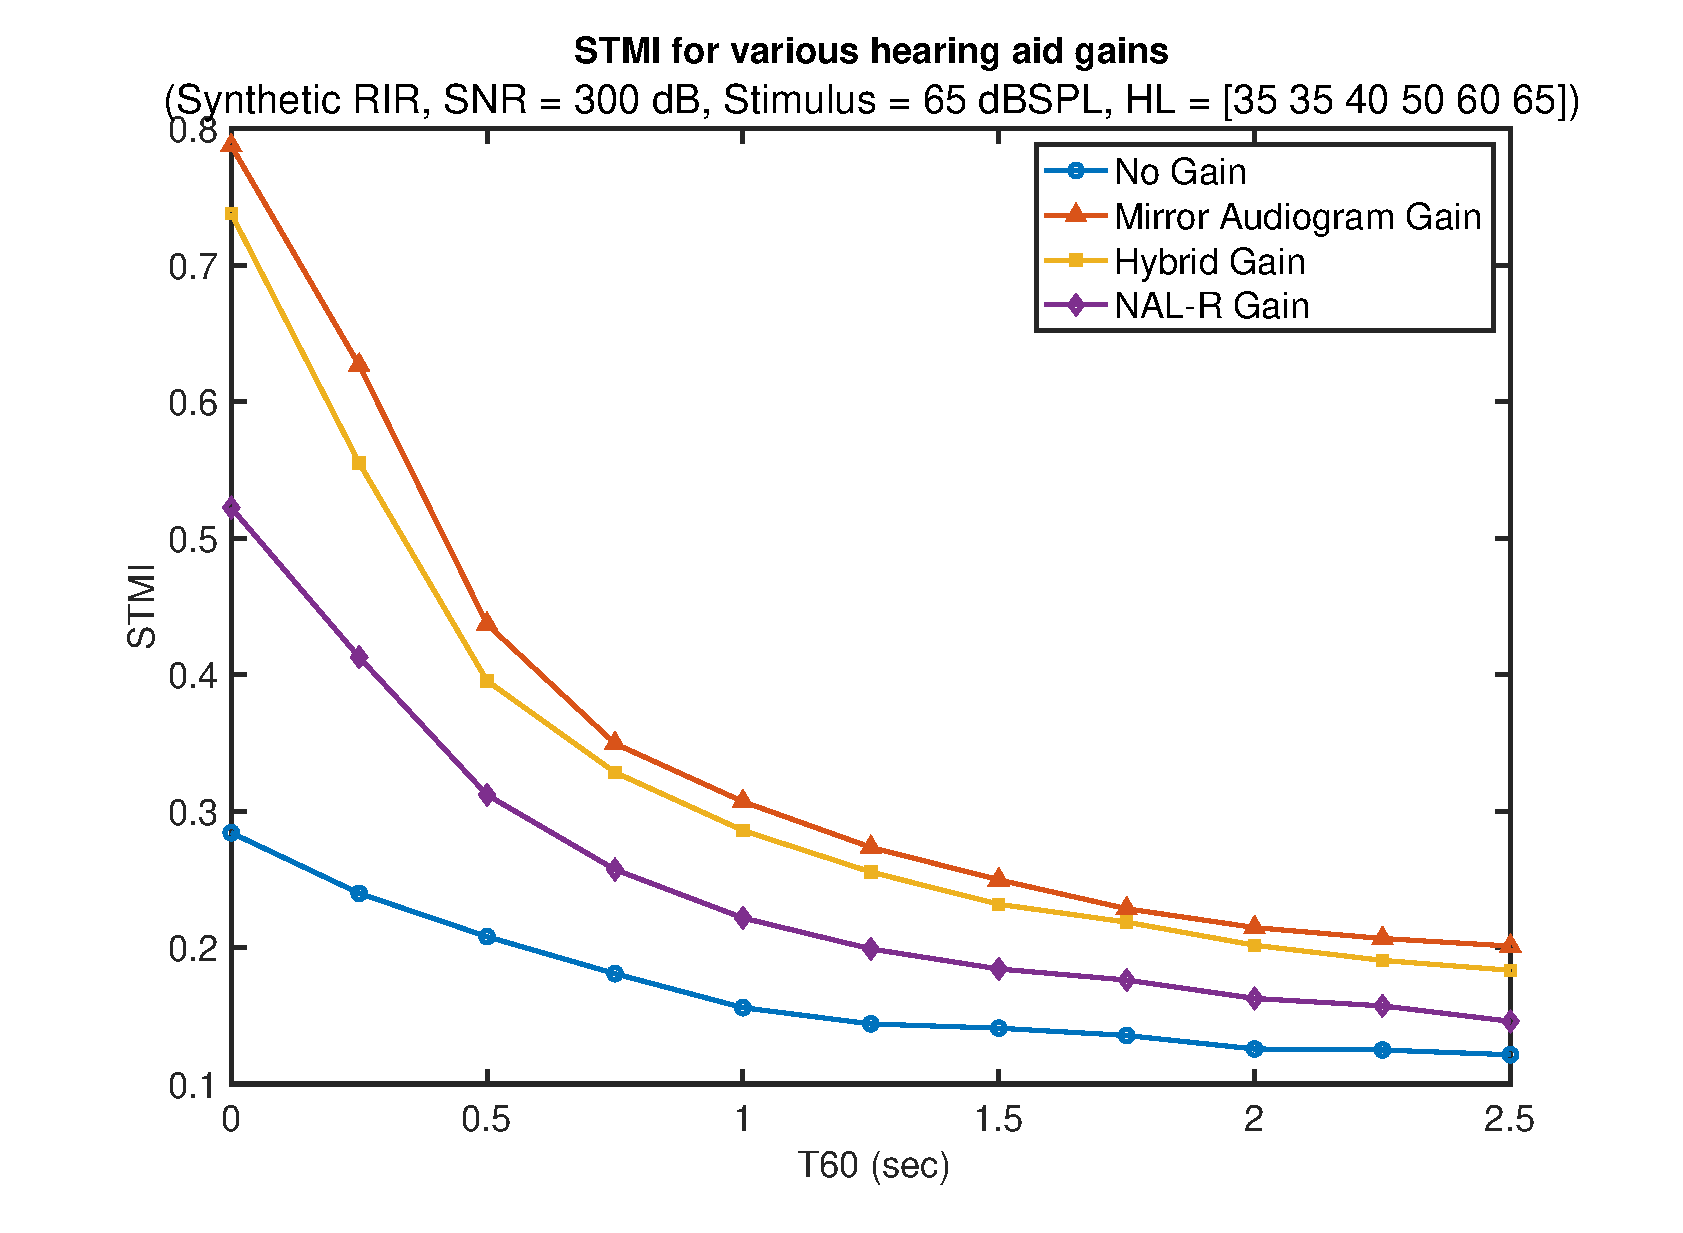
\includegraphics[width=\textwidth]{STMI_v_T60_variousHAGains}
	\end{subfigure}
	\hfill
	\caption{Comparison of perceptual benefit of four different linear hearing aid gains in the presence of reverb. Moderate high frequency hearing loss used in the perceptual models (IEC 60118-15 Moderate HL, Moderately Sloping Group), and RIRs were generated synthetically}
	\label{fig:HA_GainComparison}
\end{figure}



\subsection{Evaluation of Monaural Speech Intelligibility Metrics In Context of Reverberation}


\begin{figure}[H]
	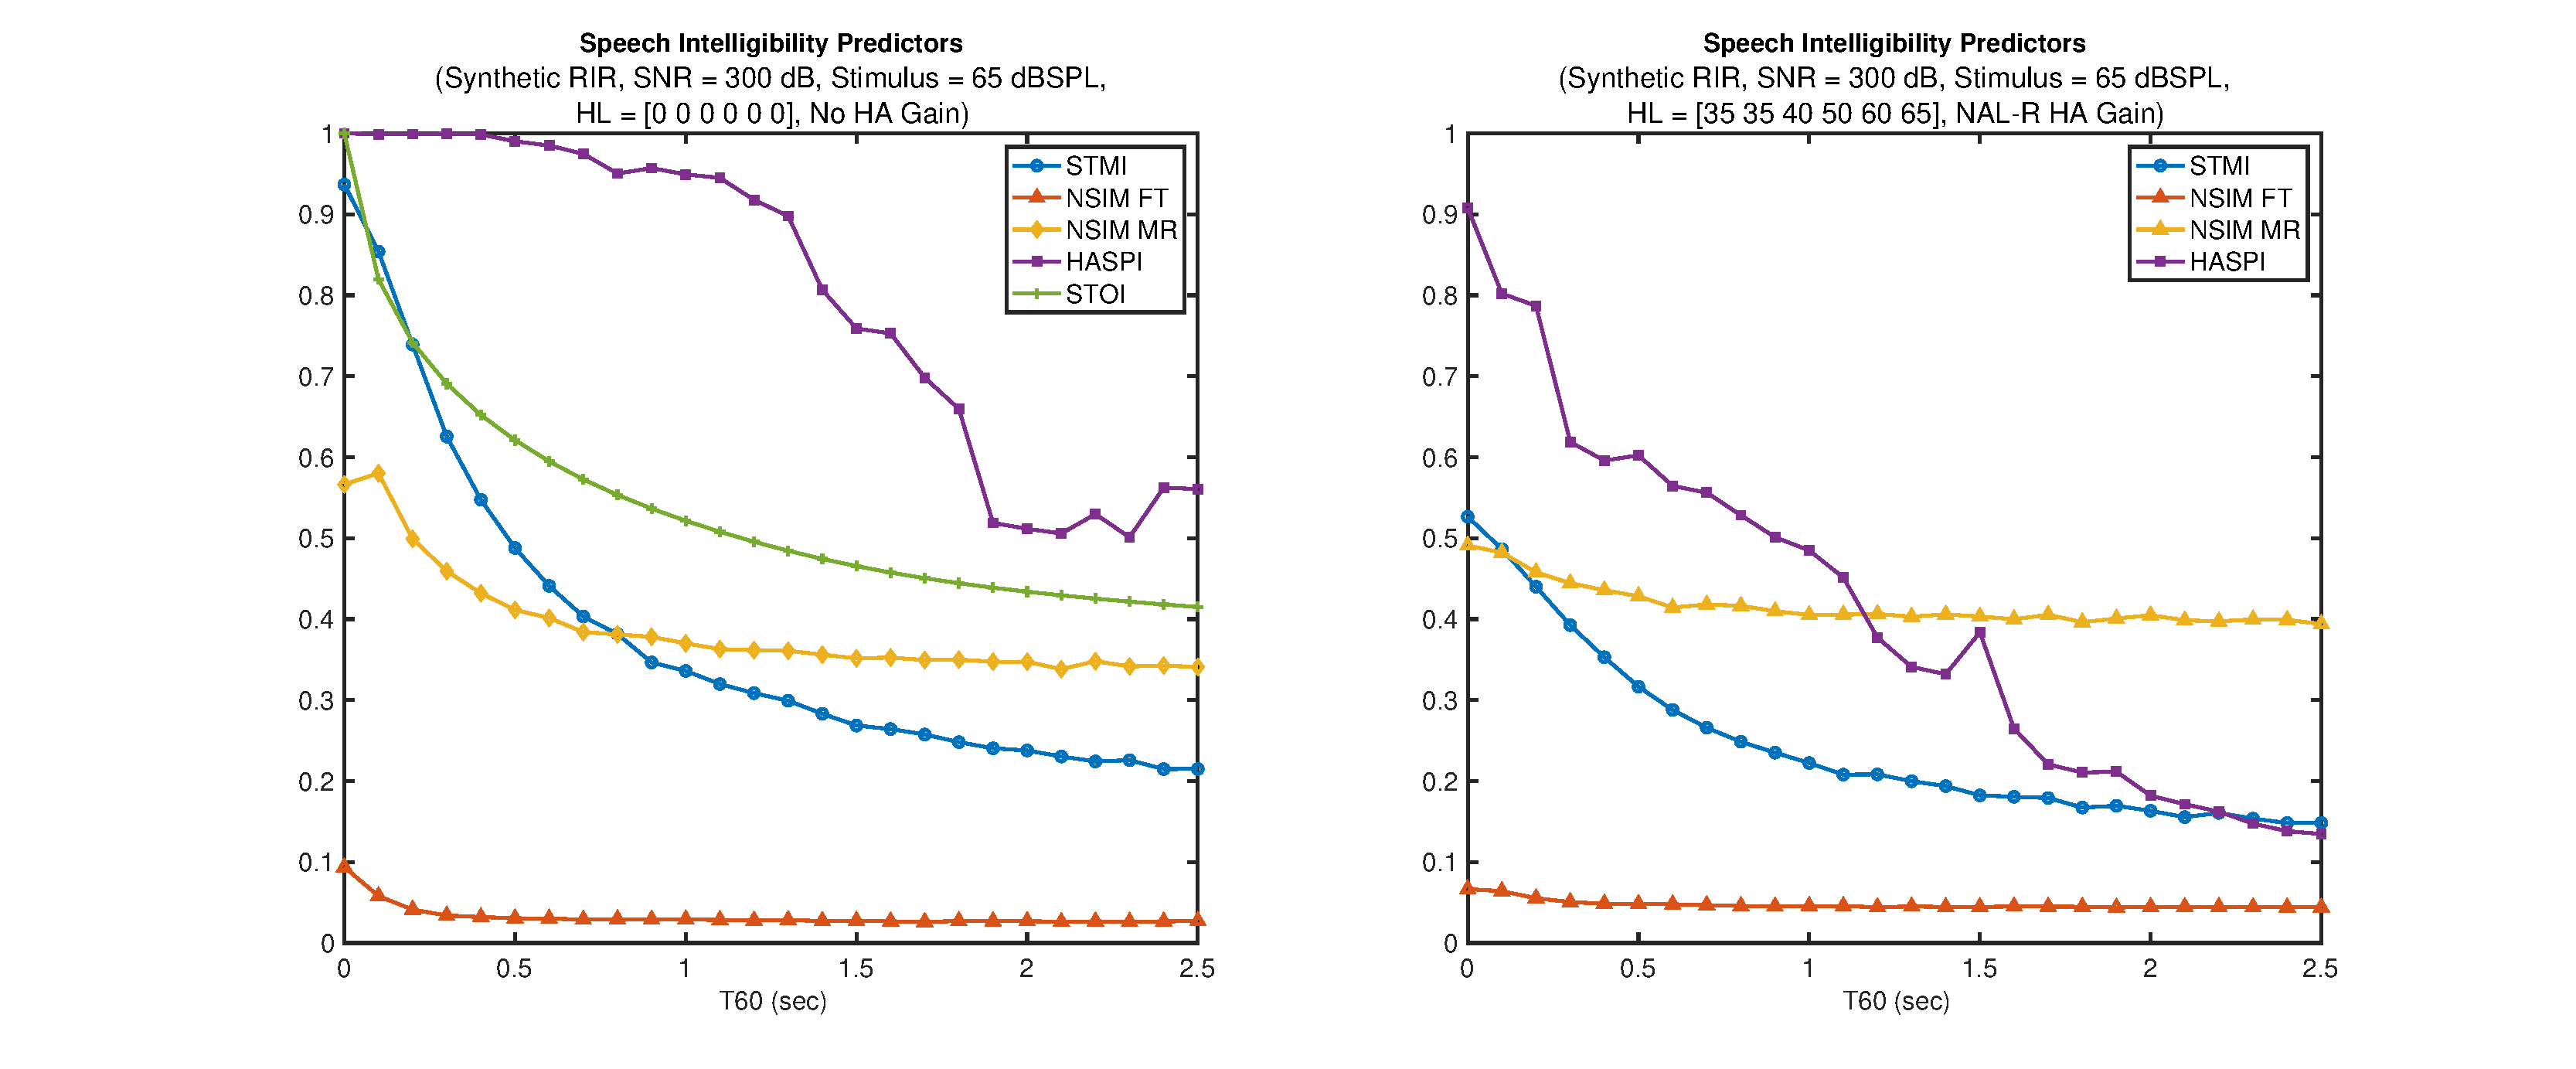
\includegraphics[width=0.98\textwidth]{SIMetricsEval_Synthetic}
	\centering
	\caption{Impact of synthetic reverberation (exponentially decaying gaussian RIRs) on SI predictors with and without hearing loss. NAL-R linear hearing aid amplification included in hearing loss case for metrics that including modeling of hearing loss}
	\label{fig:SIMetricsEval_Synthetic}
\end{figure}

\begin{figure}[H]
	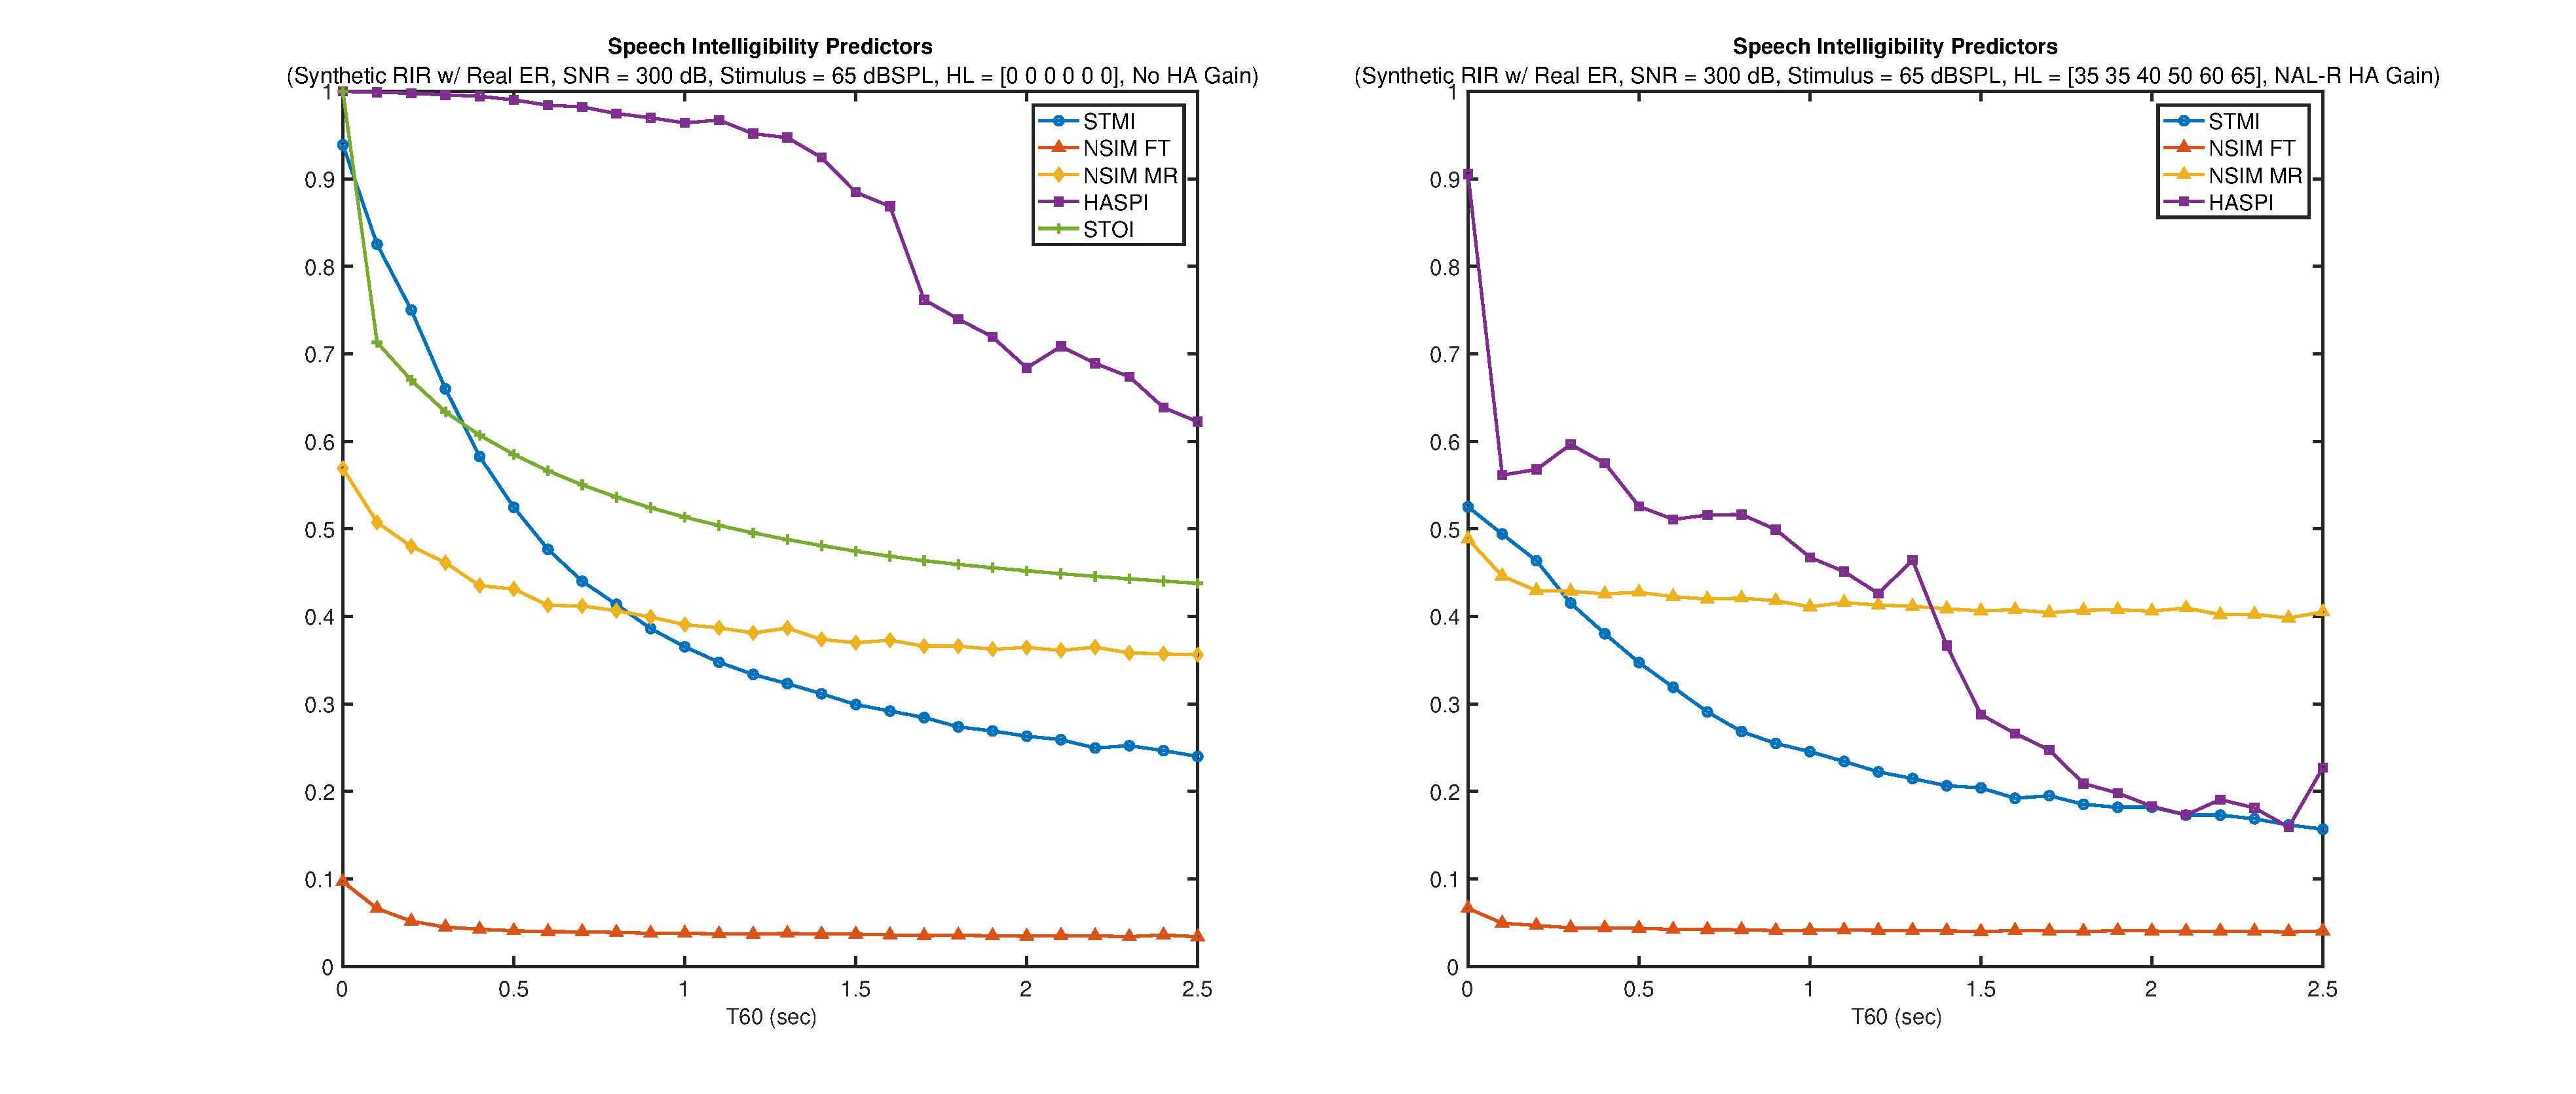
\includegraphics[width=0.98\textwidth]{SIMetricsEval_Synthetic_RealER}
	\centering
	\caption{Impact of synthetic reverberation (exponentially decaying gaussian RIRs) with added real early reflections generated by truncating a real RIR  (Office II RIR from the HRIR database) on SI predictors with and without hearing loss. NAL-R linear hearing aid amplification included in hearing loss case for metrics that including modeling of hearing loss}
	\label{fig:SIMetricsEval_Synthetic_RealER}
\end{figure}

\begin{figure}[H]
	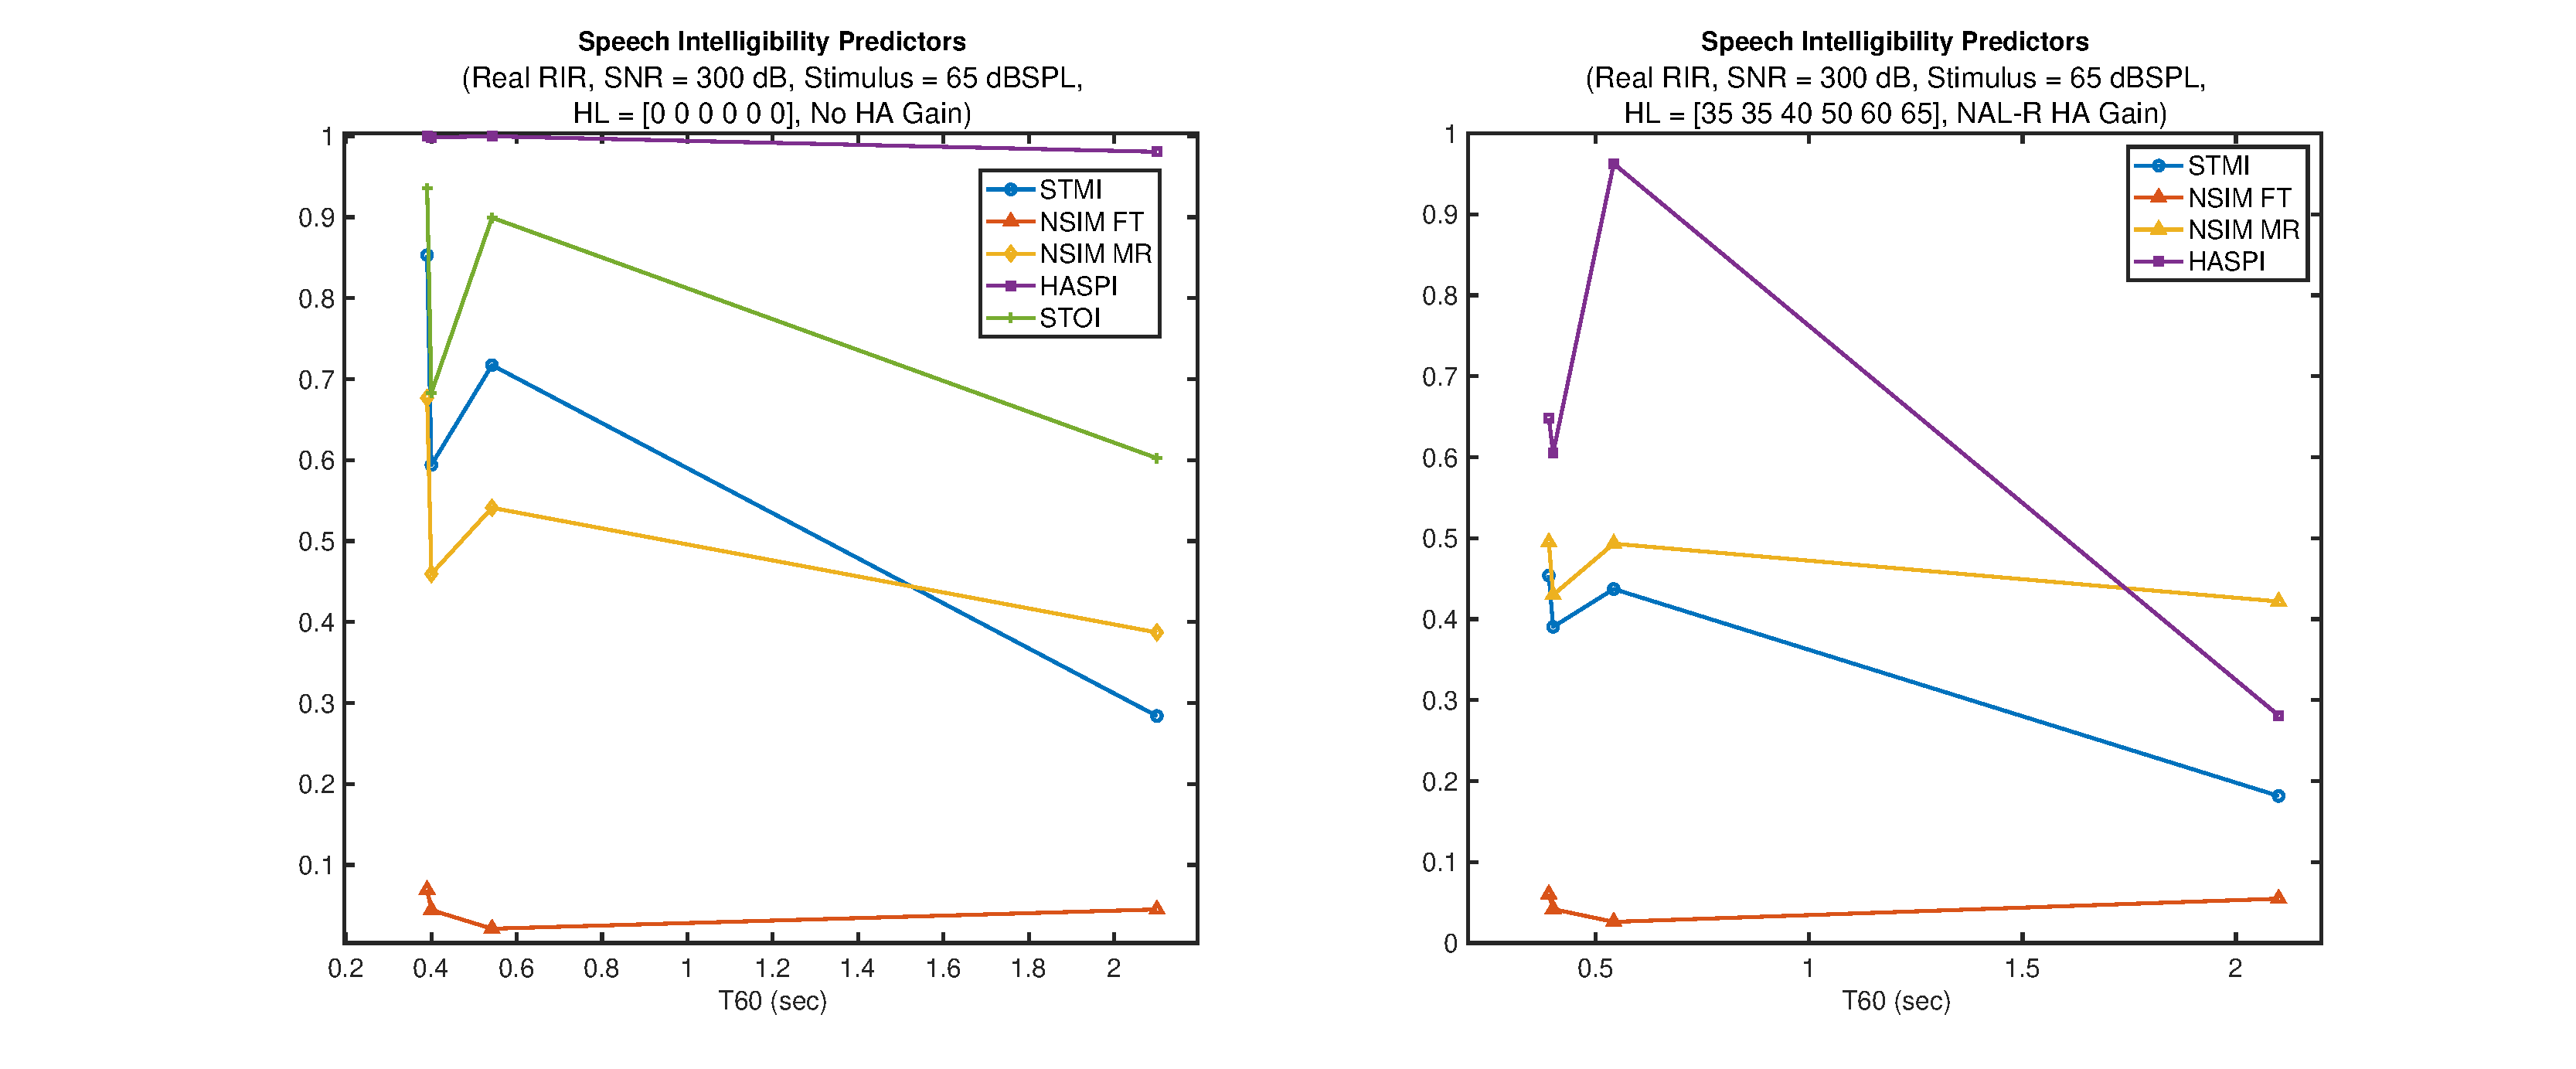
\includegraphics[width=0.98\textwidth]{SIMetricsEval_Real}
	\centering
	\caption{Impact of practical reverberation (several real measured RIRs) on SI predictors with and without hearing loss. NAL-R linear hearing aid amplification included in hearing loss case for metrics that including modeling of hearing loss}
	\label{fig:SIMetricsEval_Real}
\end{figure}

- Discussion of how SAL was truncated synthetically to control T60

\begin{figure}[H]
	\centering
	\begin{subfigure}[b]{0.49\textwidth}
		\centering
		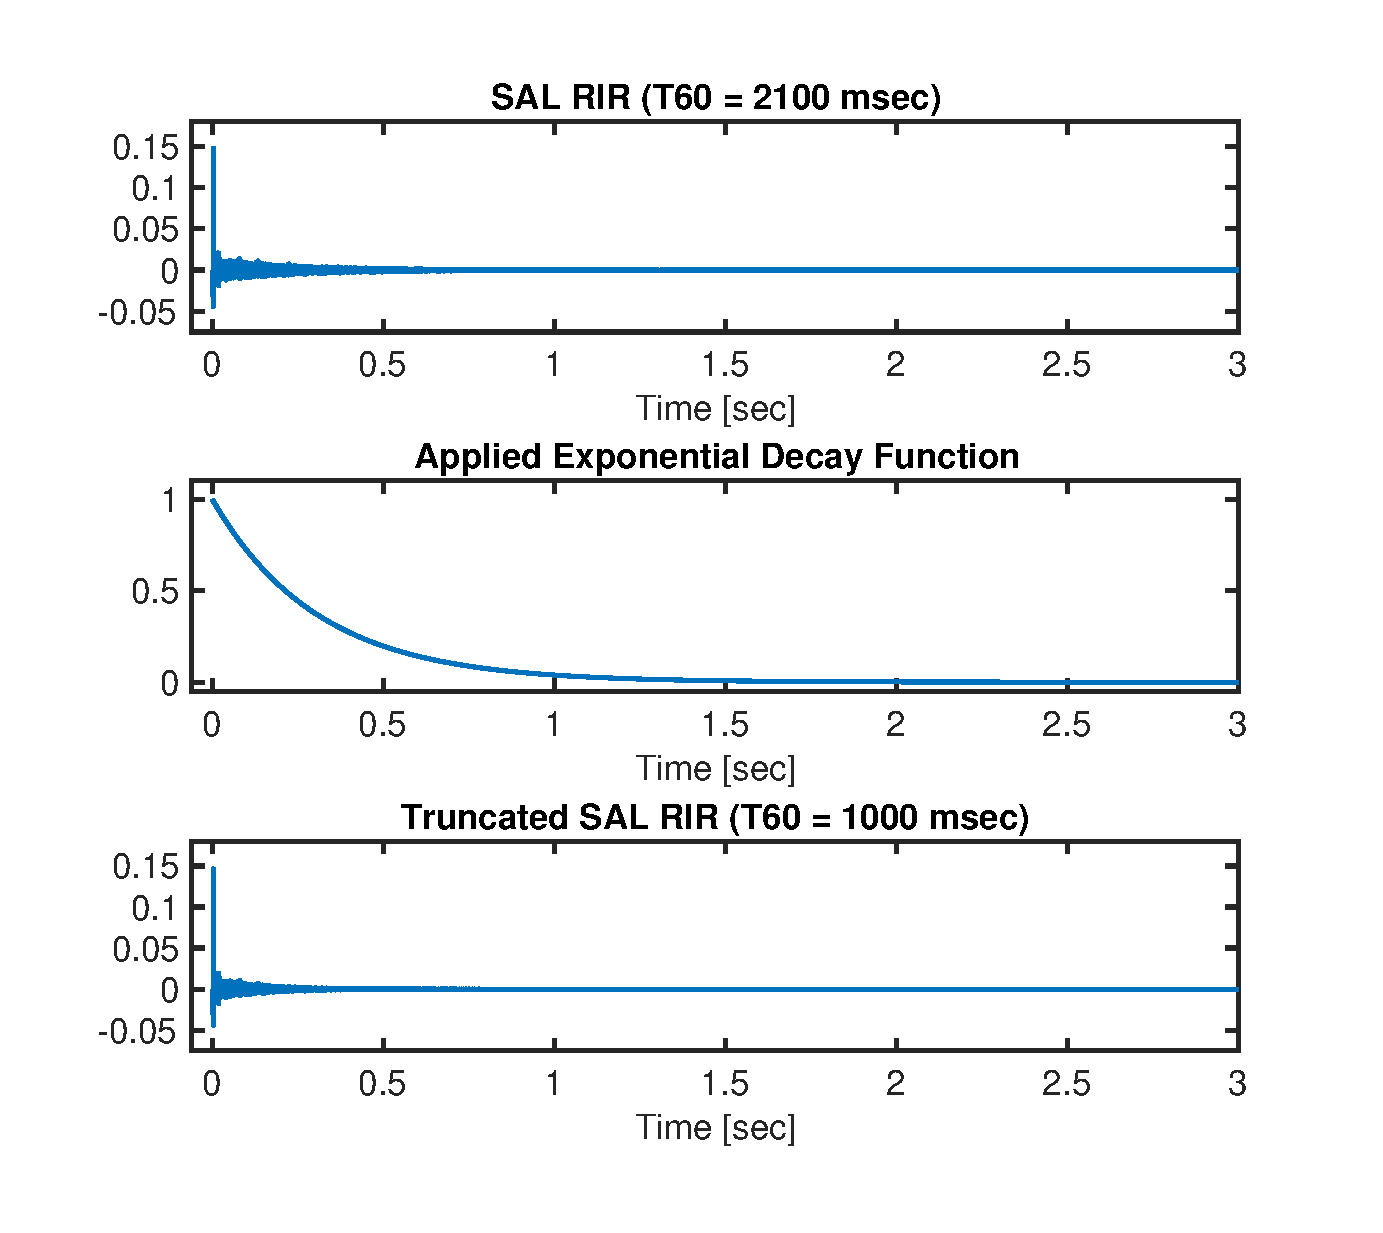
\includegraphics[width=\textwidth]{SALTruncationExample_RIR}
	\end{subfigure}
	\hfill
	\begin{subfigure}[b]{0.49\textwidth}
		\centering
		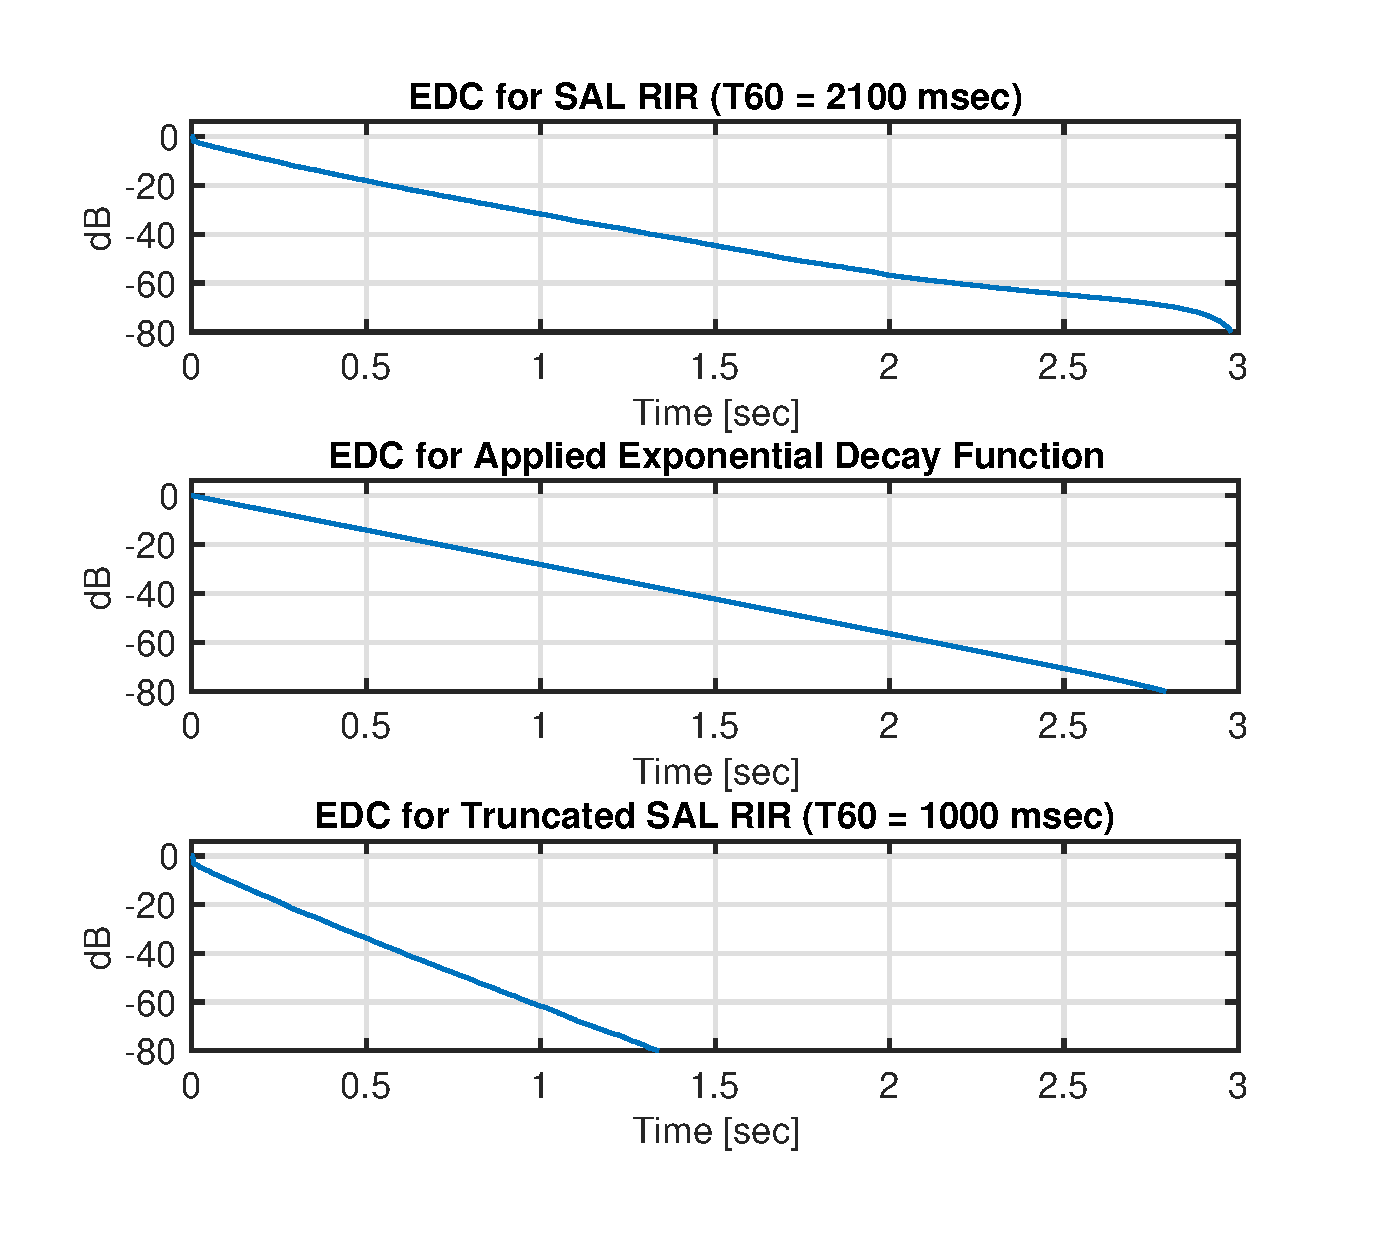
\includegraphics[width=\textwidth]{SALTruncationExample_EDC}
	\end{subfigure}
	\hfill
	\caption{TODO: REPLOT THIS WITH SAME X-AXIS USED IN ALL PLOTS FOR EDC. Example of how SAL was truncated by applying additional exponential decay as a window to manipulate T60 synthetically}
	\label{fig:SALTruncationExample}
\end{figure}

\begin{figure}[H]
	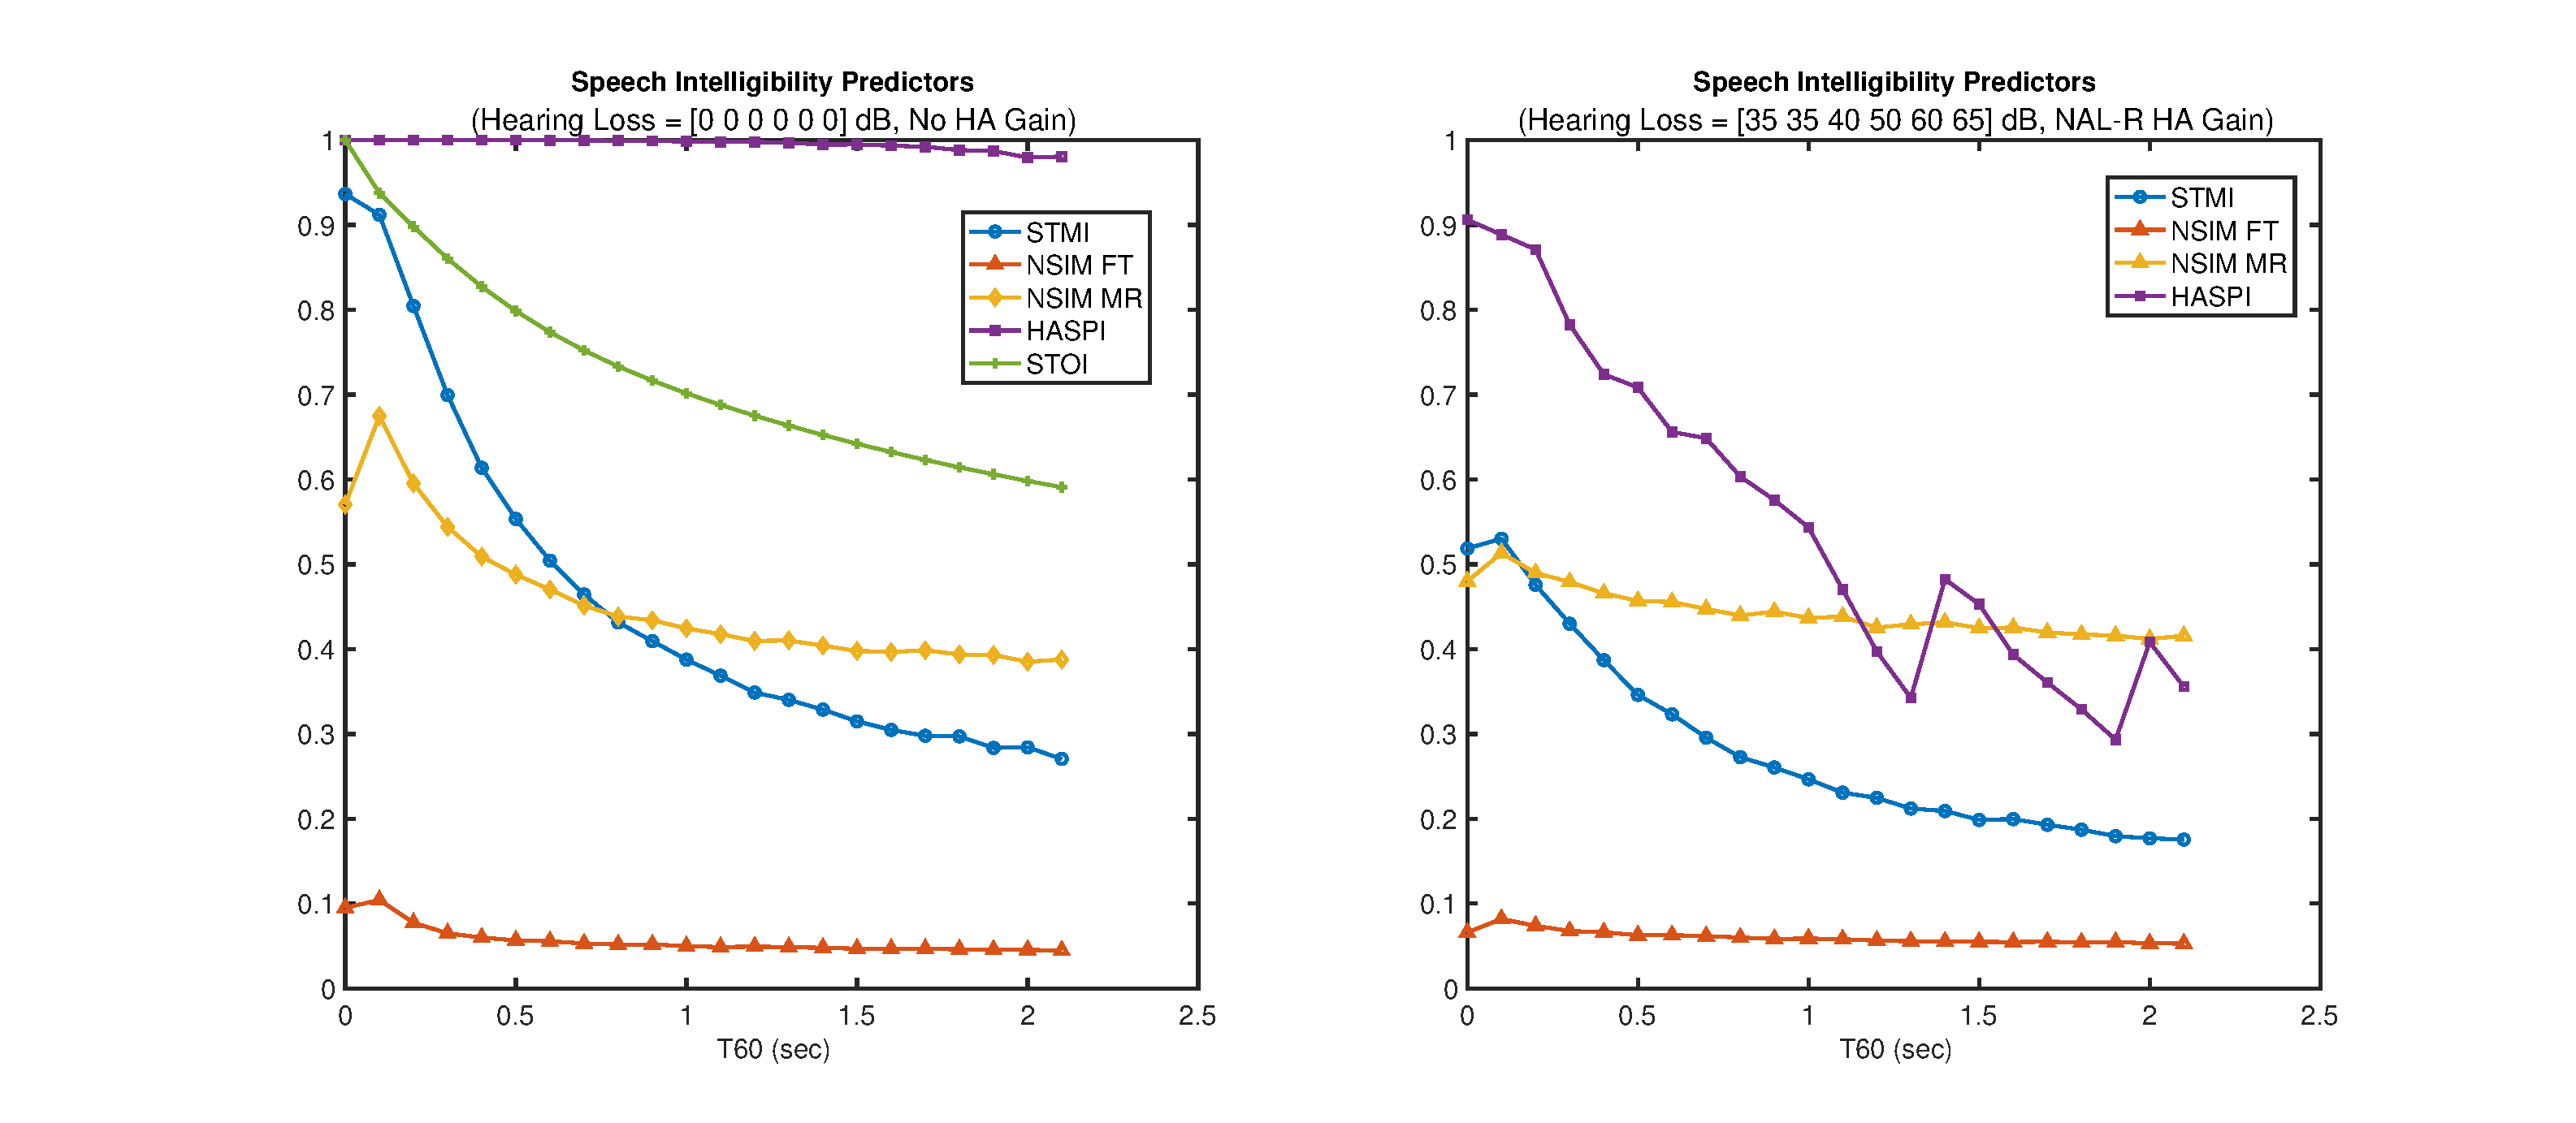
\includegraphics[width=0.98\textwidth]{SIMetricsEval_TruncatedSAL}
	\centering
	\caption{Impact of practical reverberation (SAL room from MYRiAD database exponentially truncated to control T60) on SI predictors with and without hearing loss. NAL-R linear hearing aid amplification included in hearing loss case for metrics that including modeling of hearing loss}
	\label{fig:SIMetricsEval_TruncatedSAL}
\end{figure}

- Discussion of how ER of SAL were reduced to make reverberation effect stronger


\begin{figure}[H]
	\centering
	\begin{subfigure}[b]{0.49\textwidth}
		\centering
		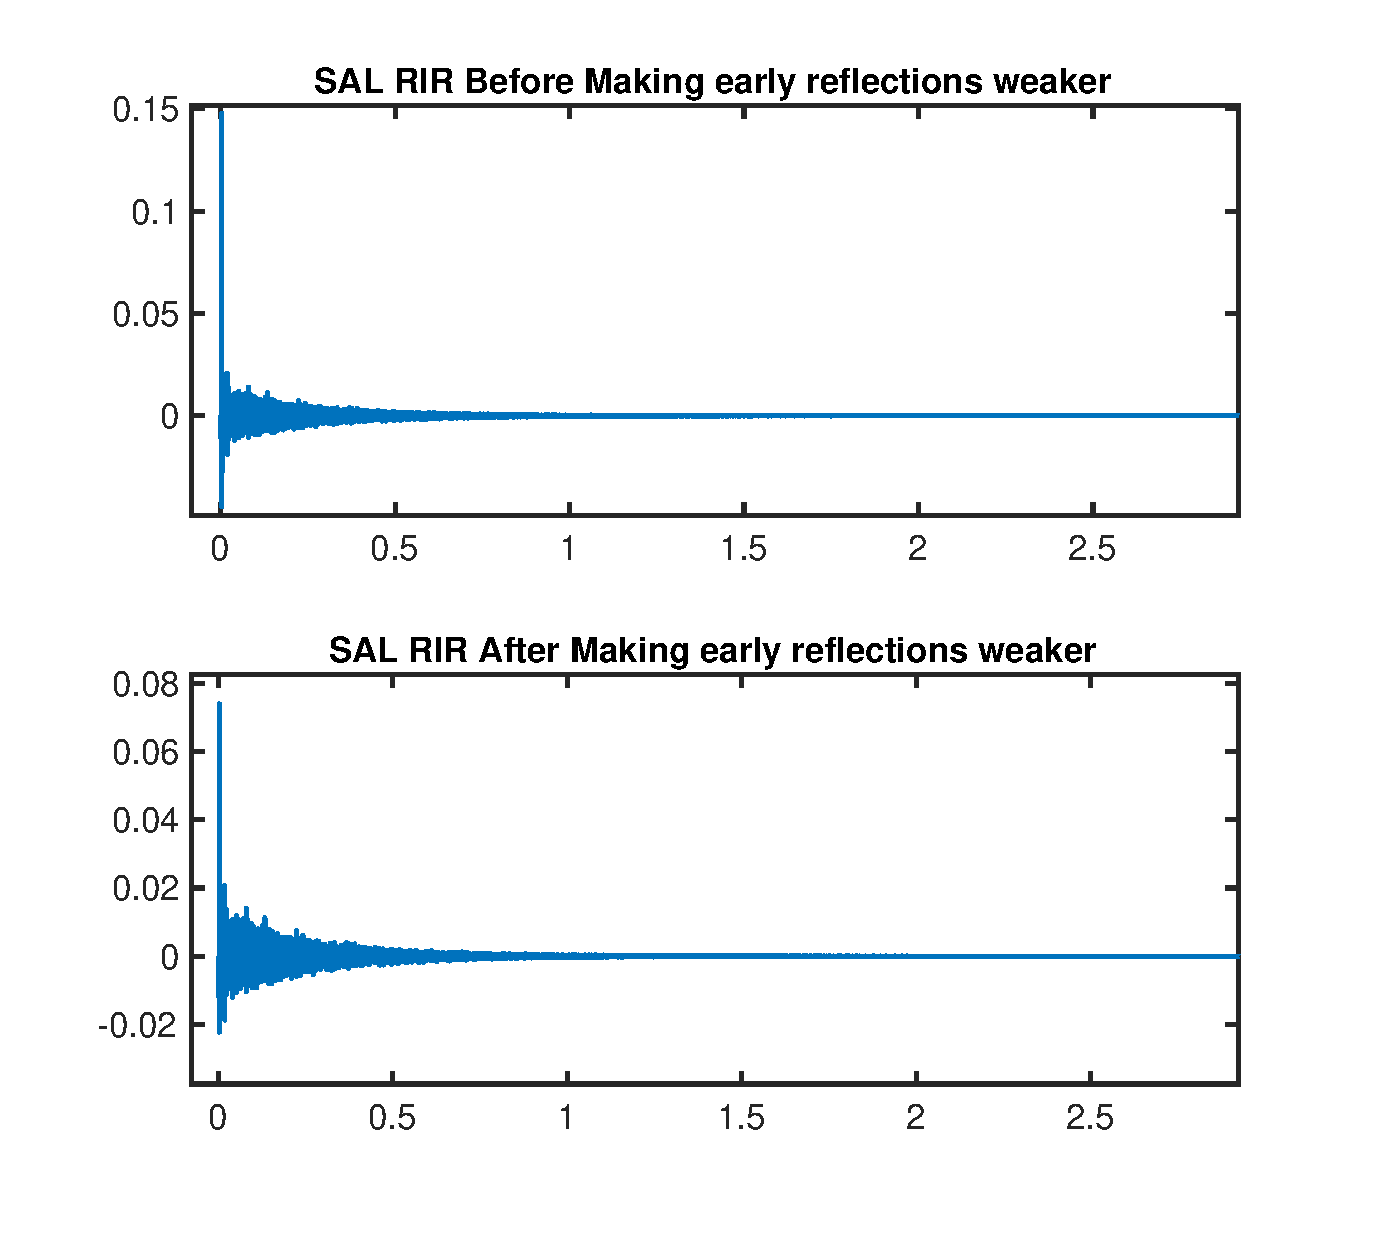
\includegraphics[width=\textwidth]{SAL_ERProcessingExample_Div2_RIR}
	\end{subfigure}
	\hfill
	\begin{subfigure}[b]{0.49\textwidth}
		\centering
		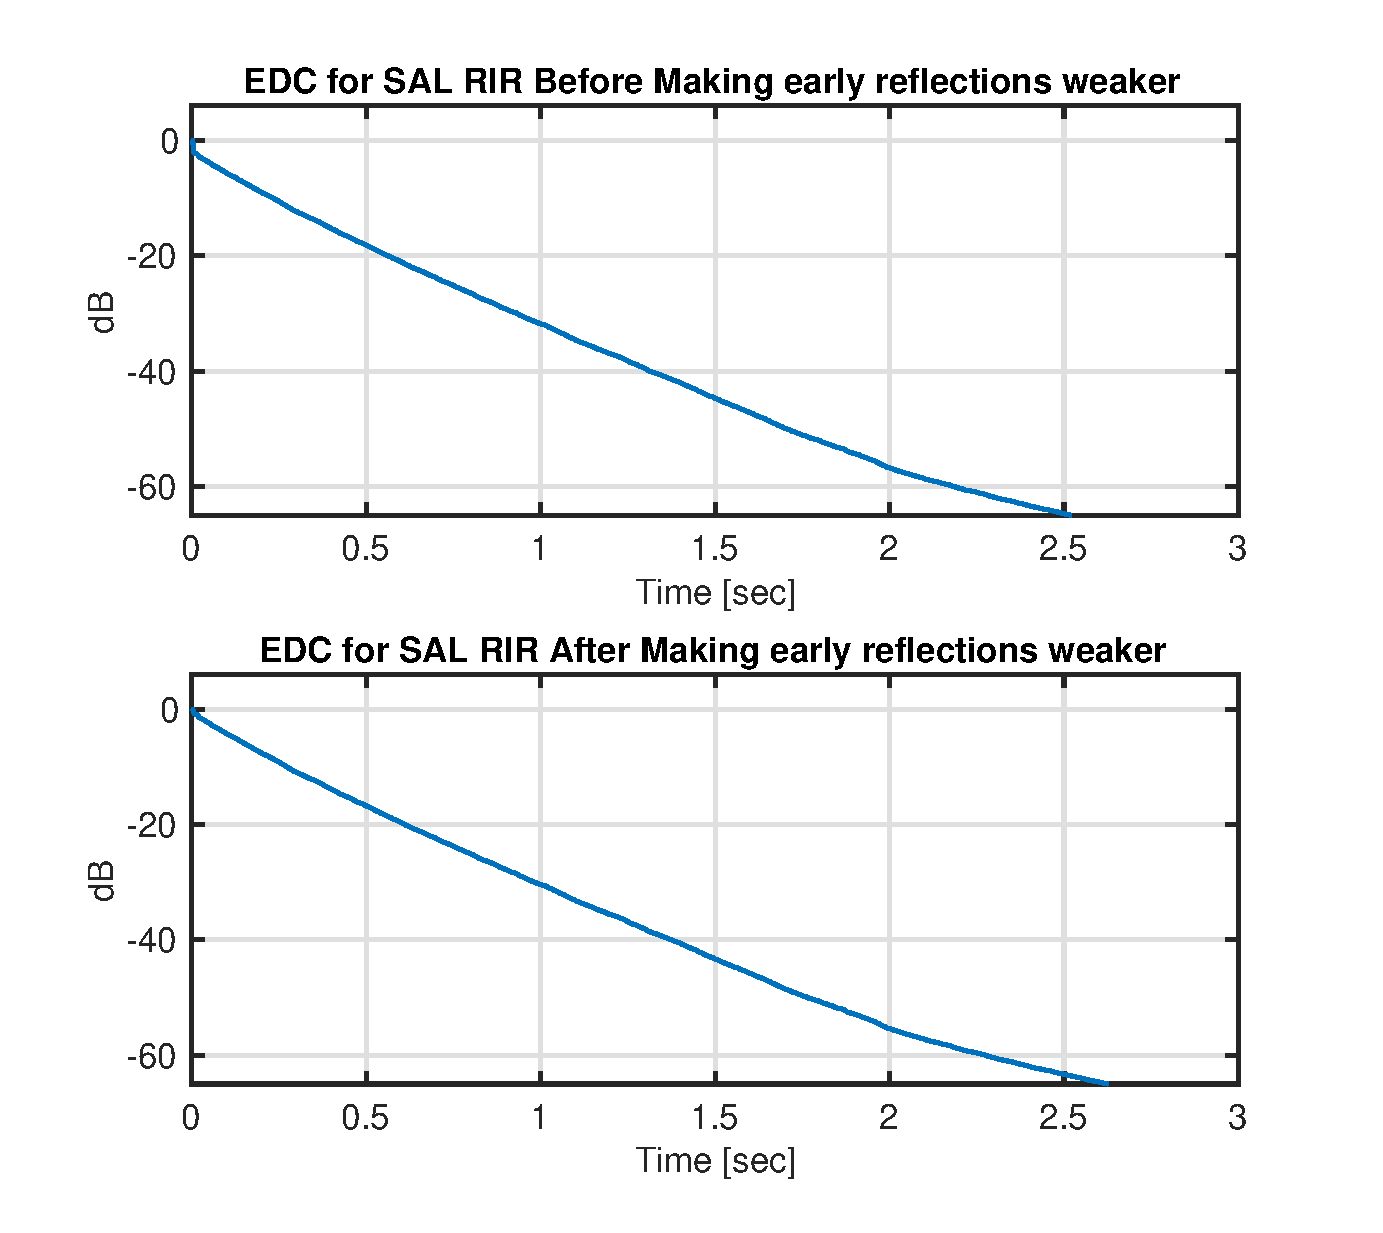
\includegraphics[width=\textwidth]{SAL_ERProcessingExample_Div2_EDC}
	\end{subfigure}
	\caption{Example of how early reflections of SAL RIR were reduced in magnitude (by 6 dB) to make reverberation effect stronger}
	\label{fig:SAL_ERProcessing_Div2}
\end{figure}

\begin{figure}[H]
	\centering
	\begin{subfigure}[b]{0.98\textwidth}
		\centering
		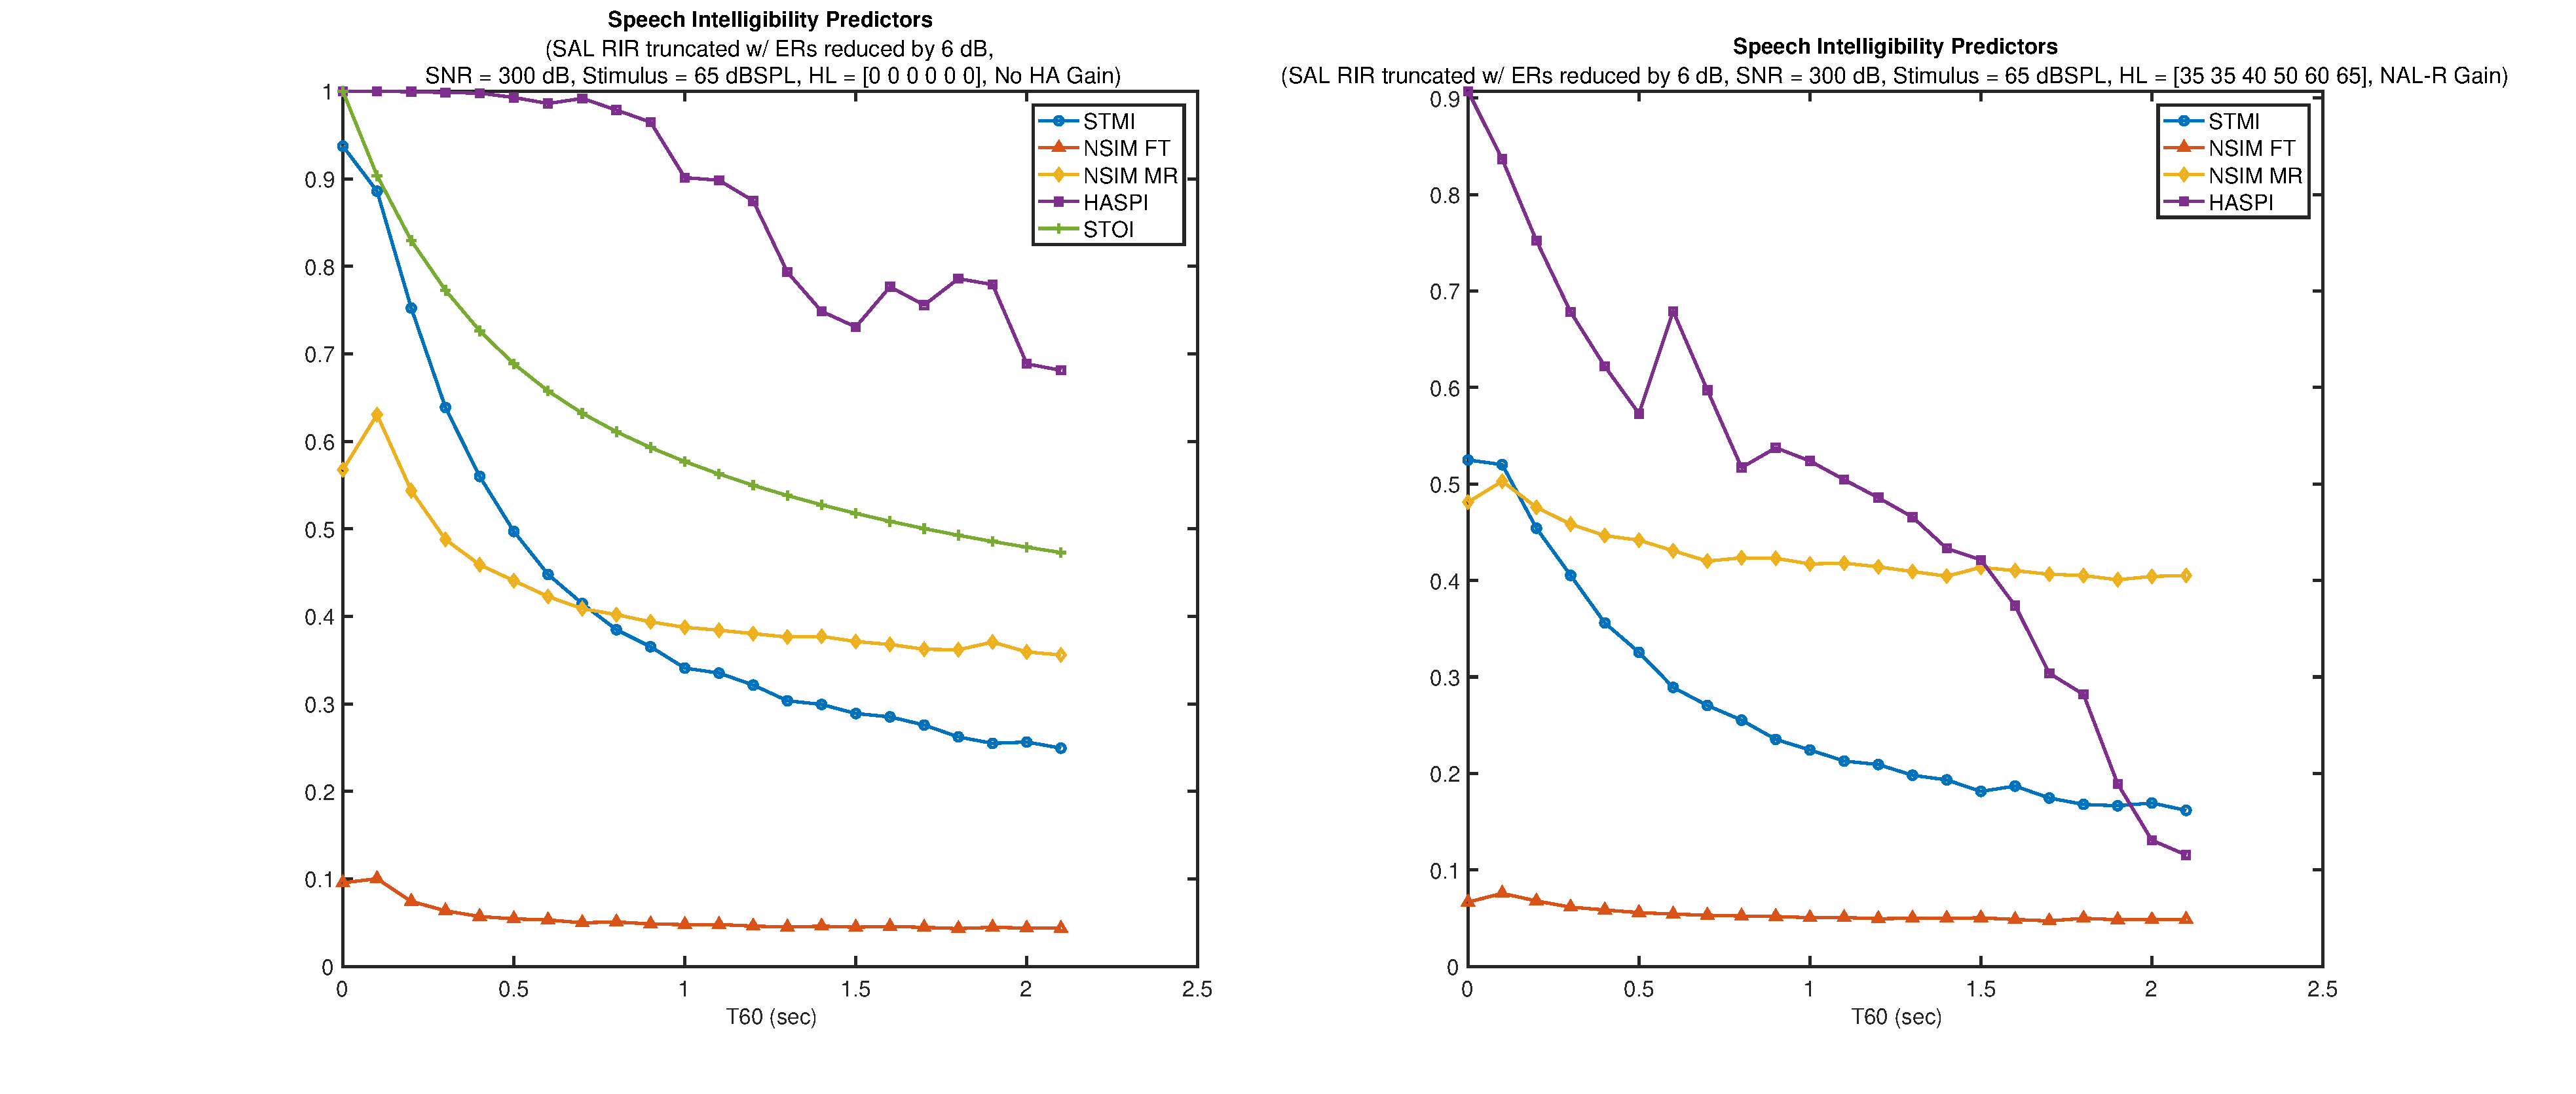
\includegraphics[width=\textwidth]{SAL_ERProcessingExample_Div2_SI}
	\end{subfigure}
	\caption{Impact of reducing early reflections of SAL RIR (i.e., Figure \ref{fig:SAL_ERProcessing_Div2}). SI shown before RIR processing (left) and after RIR processing (right) for comparison}
\label{fig:SAL_ERProcessing_Div2_SI_Results}
\end{figure}


- Discussion of how T60 is not a complete picture of the effects of reverb, EDT and SI together provide a more complete description. Generally speaking these are both encapsulated collectively in DRR

- Discussion of how NSIM and STMI continue to increase where HASPI plateaus suggesting that they can be used to reflect listening effort (NSIM and STMI still have some saturation, but not as much as subjective speech intelligibility). NSIM, STMI have no explicit application of a nonlinear  P/I function to map to SI, see notes about on how P/I function varies greatly depending on many factors so cant really be universal. The exact value of NSIM and STMI is not as meaningful, its moreso the how it changes with respect to control variables

- HASPI is mapped to SI, but I dont think it has an explicity P/I function -- not clear need to investigate. It clearly does strongly saturate in a way the resembles subjective SI more accurately

- Discussion of how NSIM and STMI were scaled (with a constant scaling factor accross all plots) to better view the trends accross all metrics on the same plot.

\begin{figure}[H]
	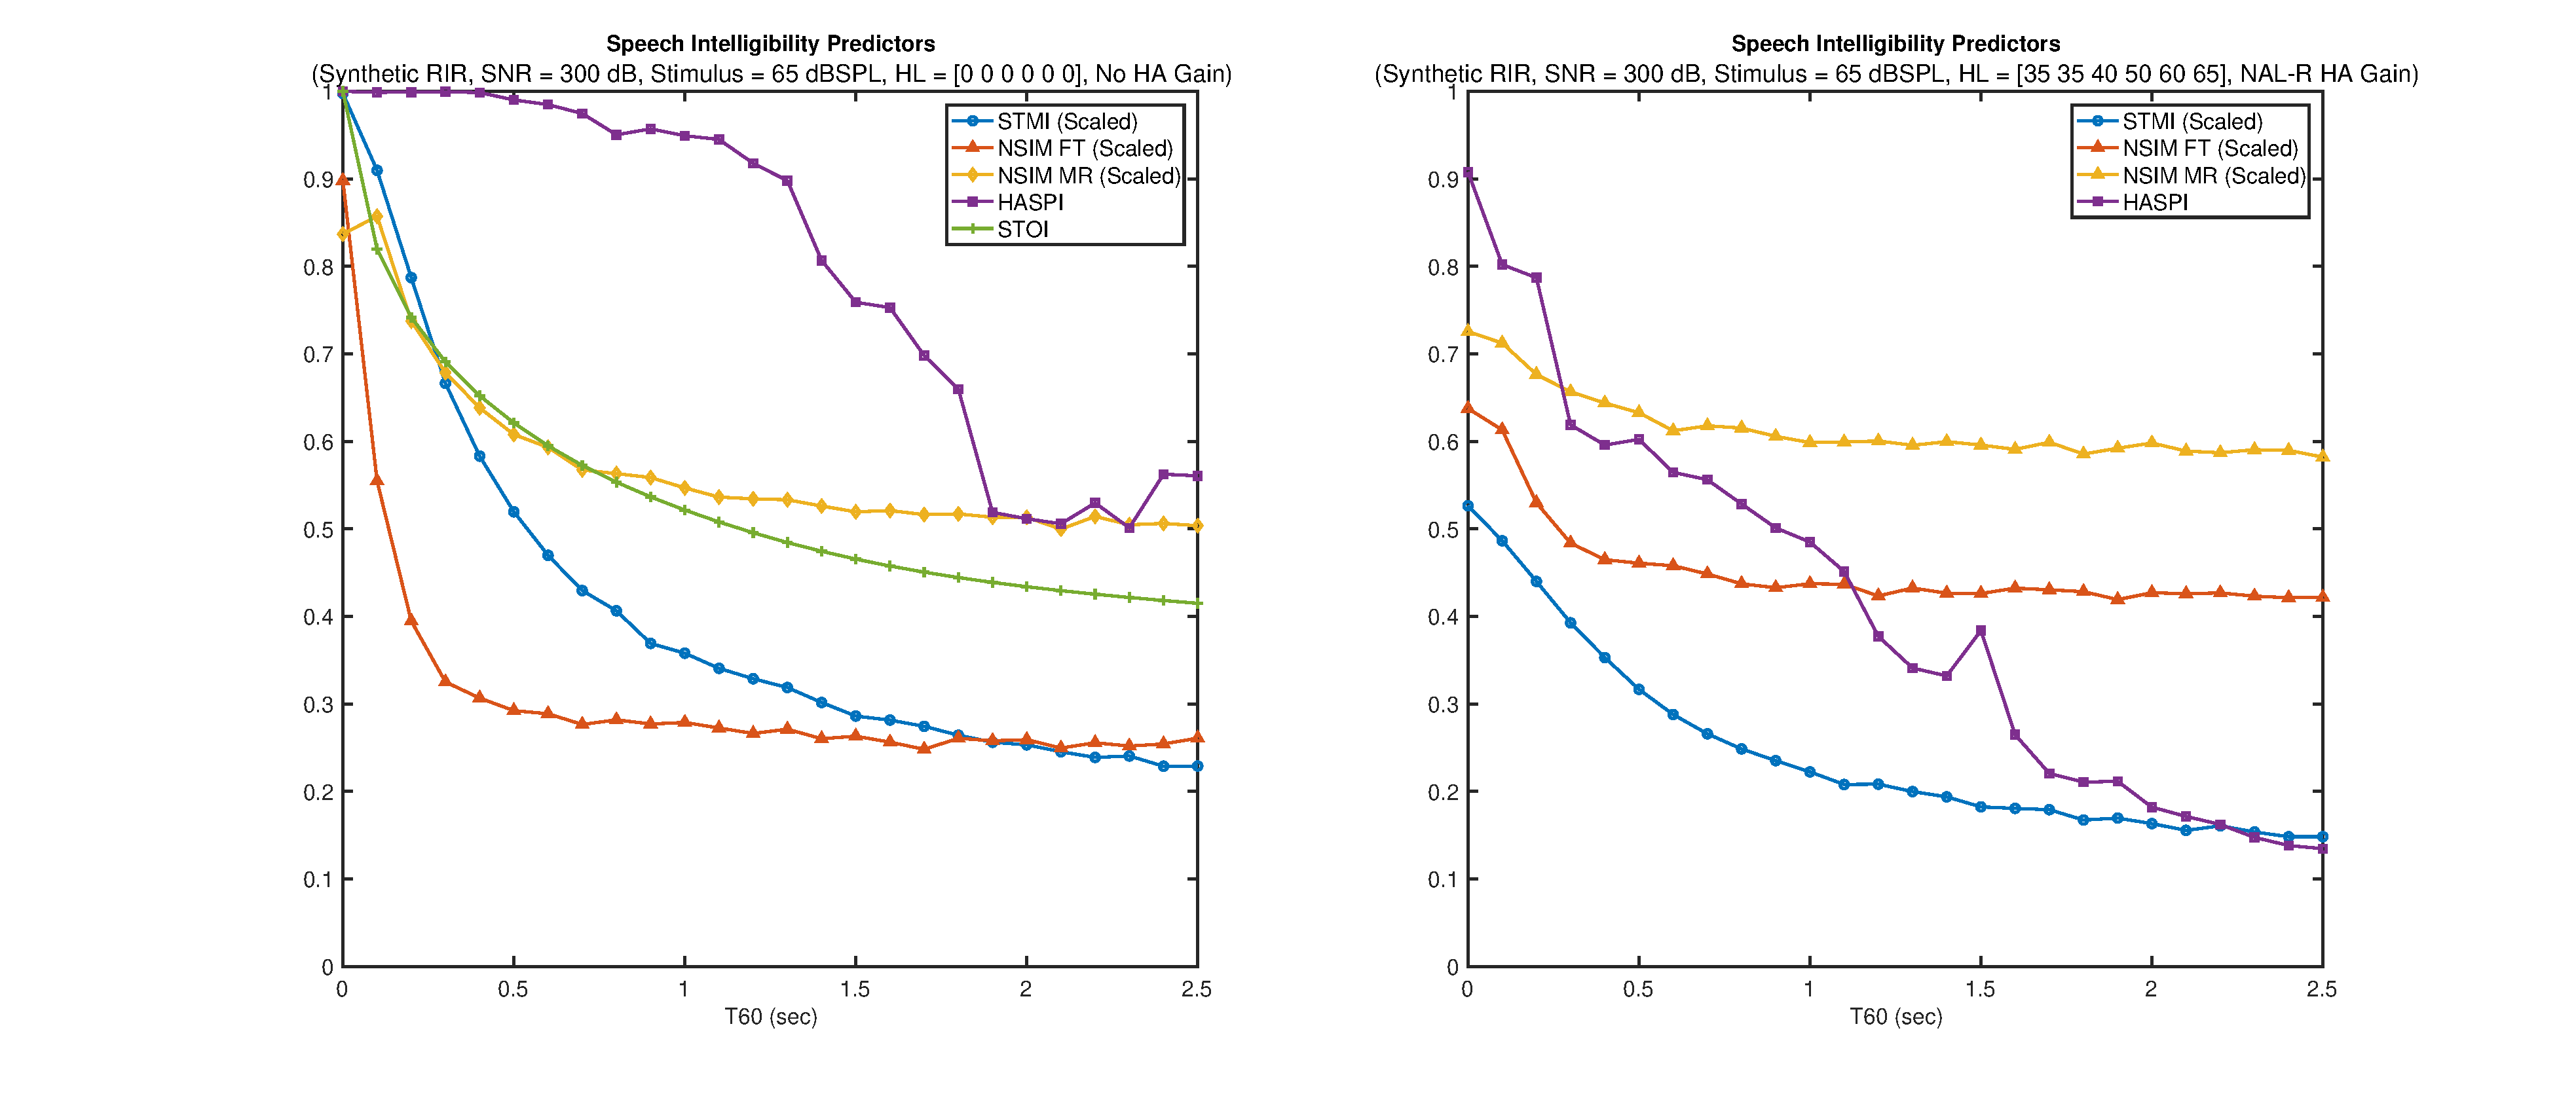
\includegraphics[width=0.98\textwidth]{SIMetricsEval_Synthetic_wScaling}
	\centering
	\caption{Impact of synthetic reverberation (exponentially decaying gaussian RIRs) on SI predictors with and without hearing loss. NAL-R linear hearing aid amplification included in hearing loss case for metrics that including modeling of hearing loss. Scaling applied to NSIM and STMI values to better view all metrics on the same plot.}
	\label{fig:SIMetricsEval_Synthetic_wScaling}
\end{figure}

\begin{figure}[H]
	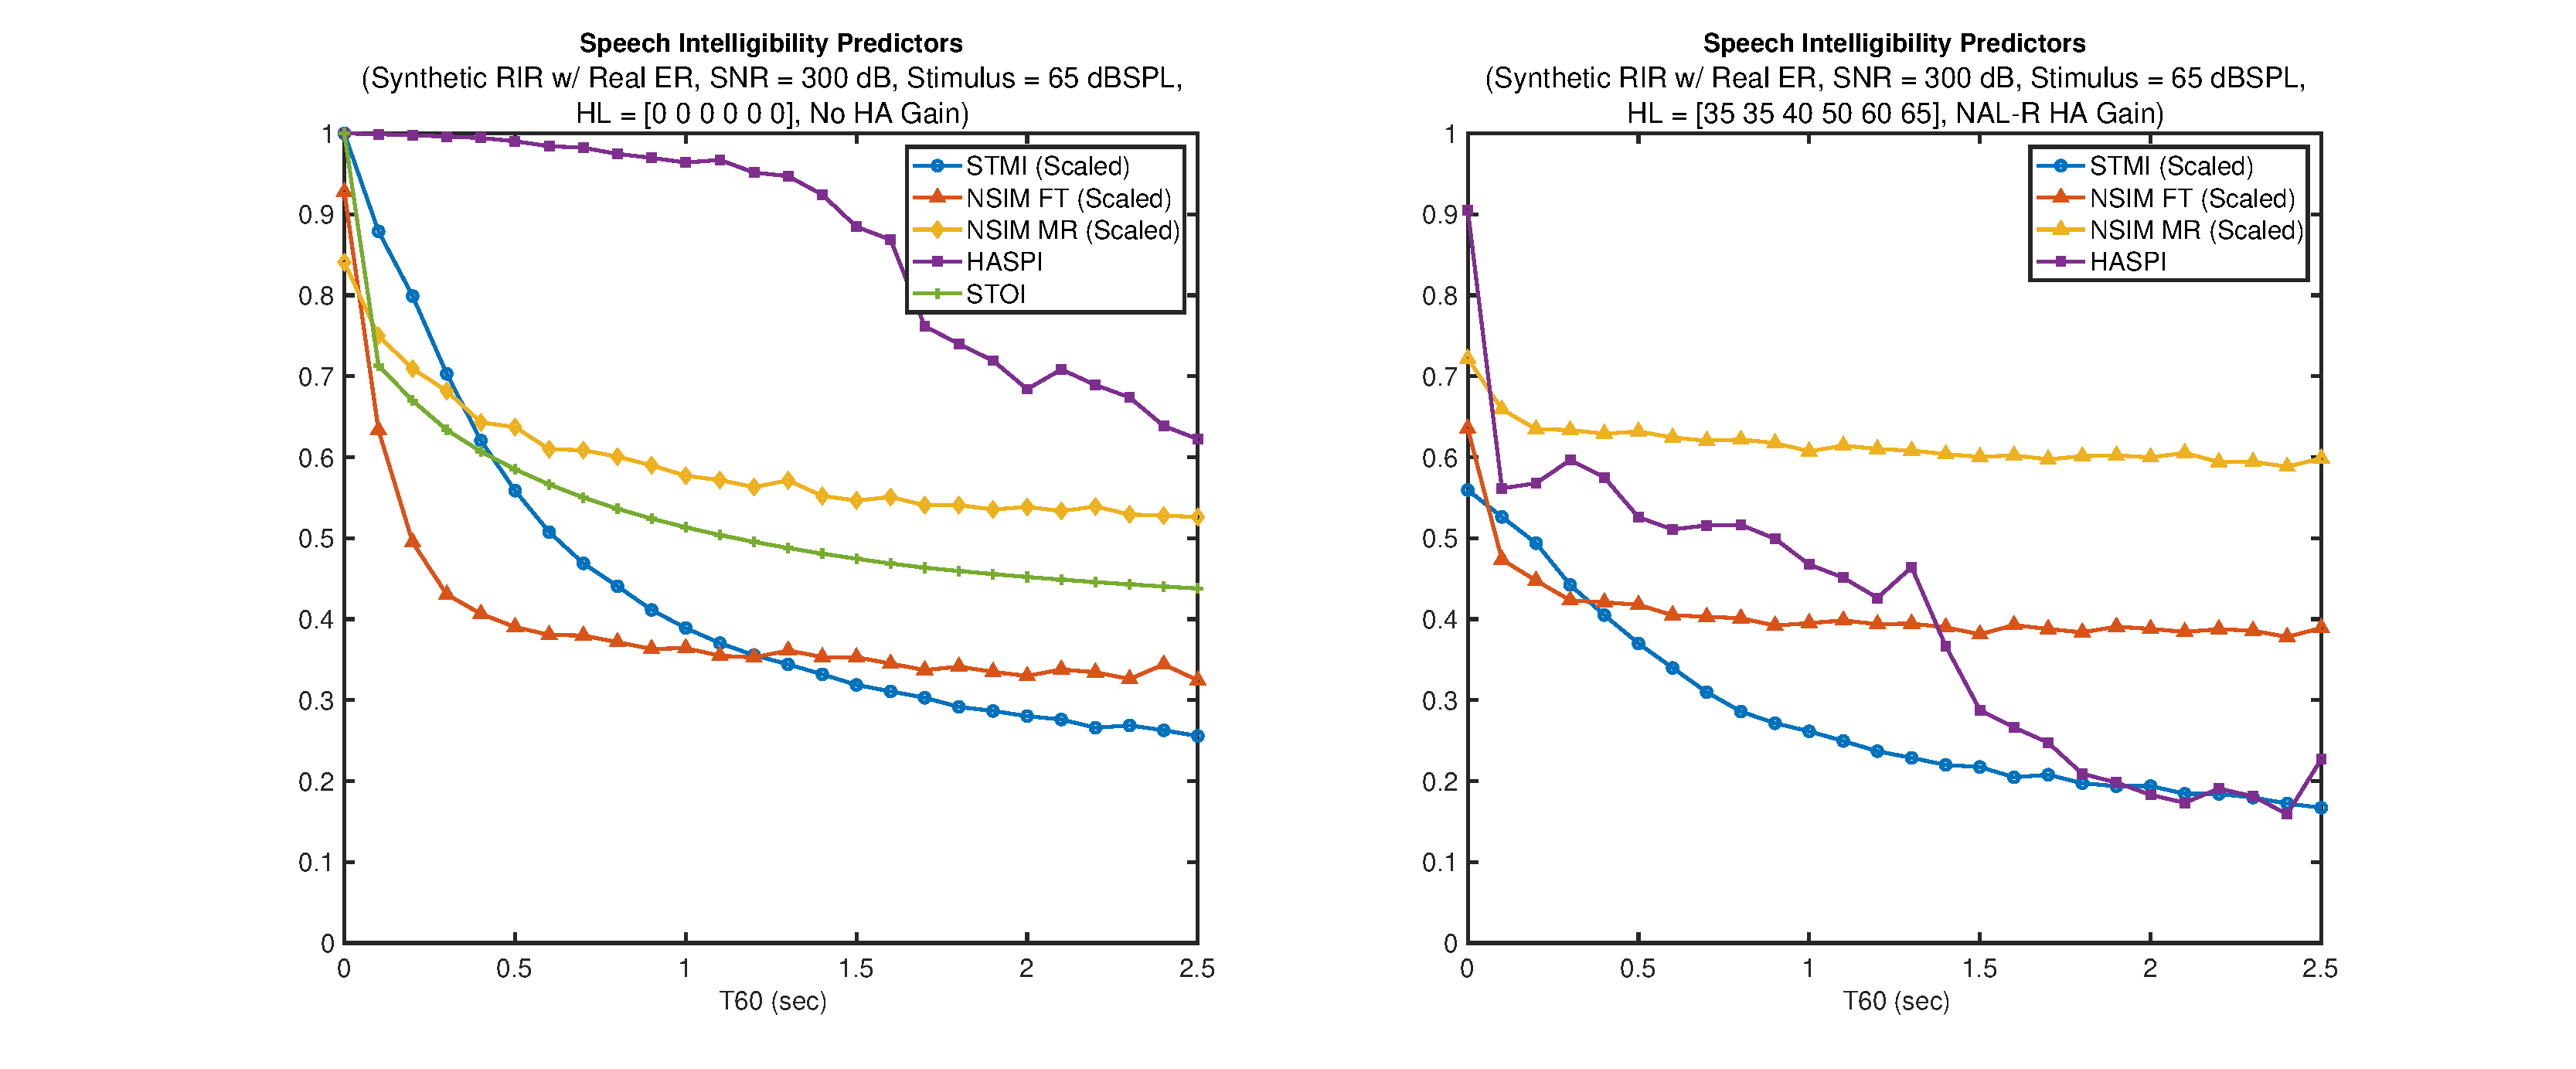
\includegraphics[width=0.98\textwidth]{SIMetricsEval_Synthetic_RealER_wScaling}
	\centering
	\caption{Impact of synthetic reverberation (exponentially decaying gaussian RIRs) with added real early reflections generated by truncating a real RIR  (Office II RIR from the HRIR database) on SI predictors with and without hearing loss. NAL-R linear hearing aid amplification included in hearing loss case for metrics that including modeling of hearing loss. Scaling applied to NSIM and STMI values to better view all metrics on the same plot.}
	\label{fig:SIMetricsEval_Synthetic_RealER_wScaling}
\end{figure}

\begin{figure}[H]
	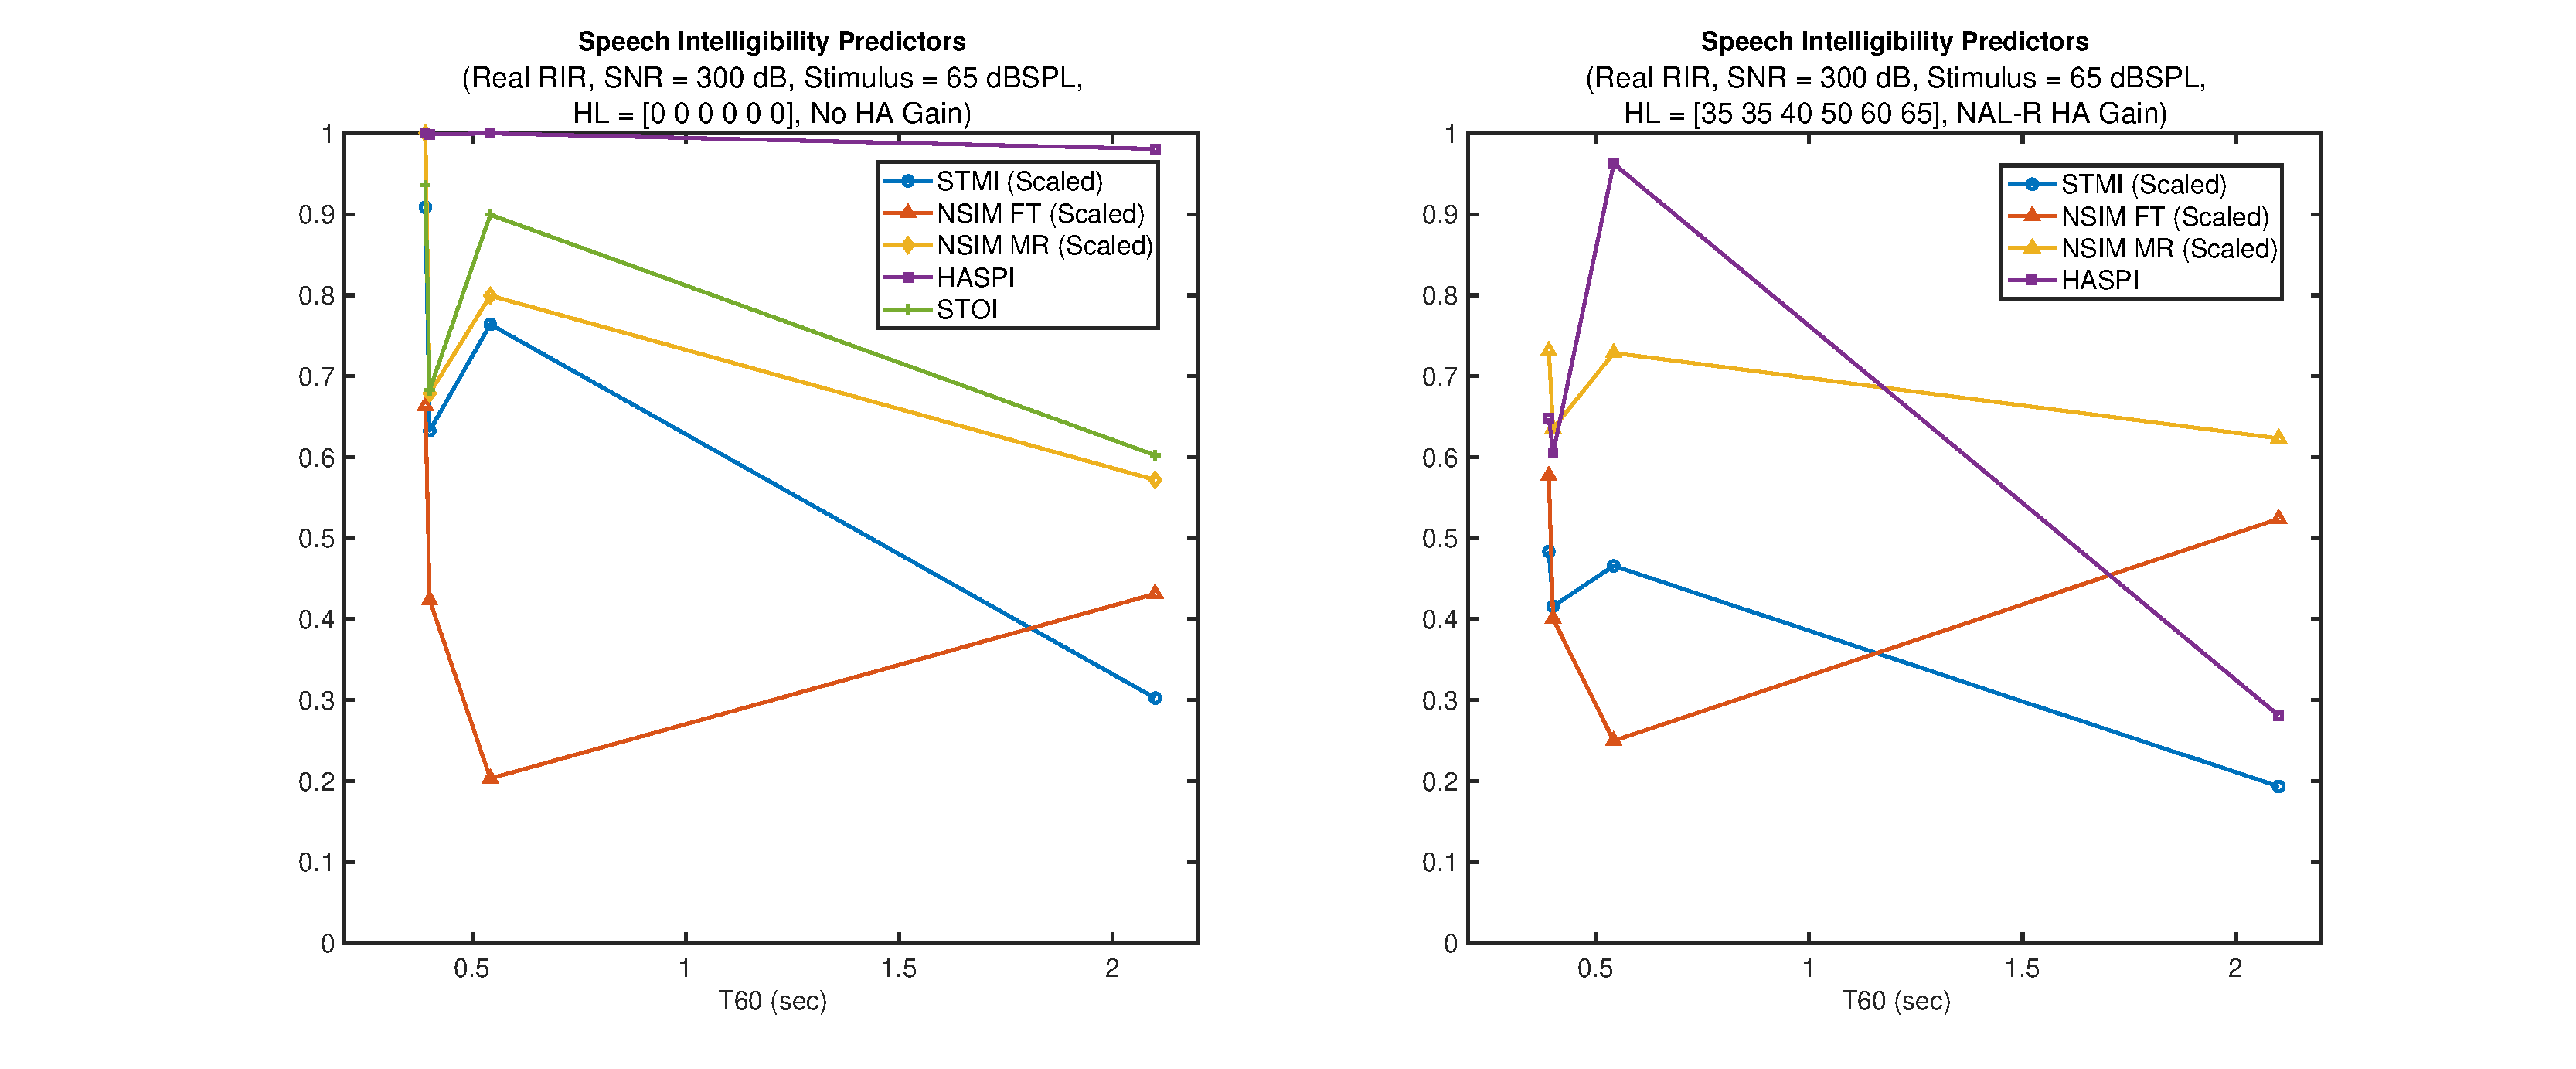
\includegraphics[width=0.98\textwidth]{SIMetricsEval_Real_wScaling}
	\centering
	\caption{Impact of practical reverberation (several real measured RIRs) on SI predictors with and without hearing loss. NAL-R linear hearing aid amplification included in hearing loss case for metrics that including modeling of hearing loss.  Scaling applied to NSIM and STMI values to better view all metrics on the same plot.}
	\label{fig:SIMetricsEval_Real_wScaling}
\end{figure}

\begin{figure}[H]
	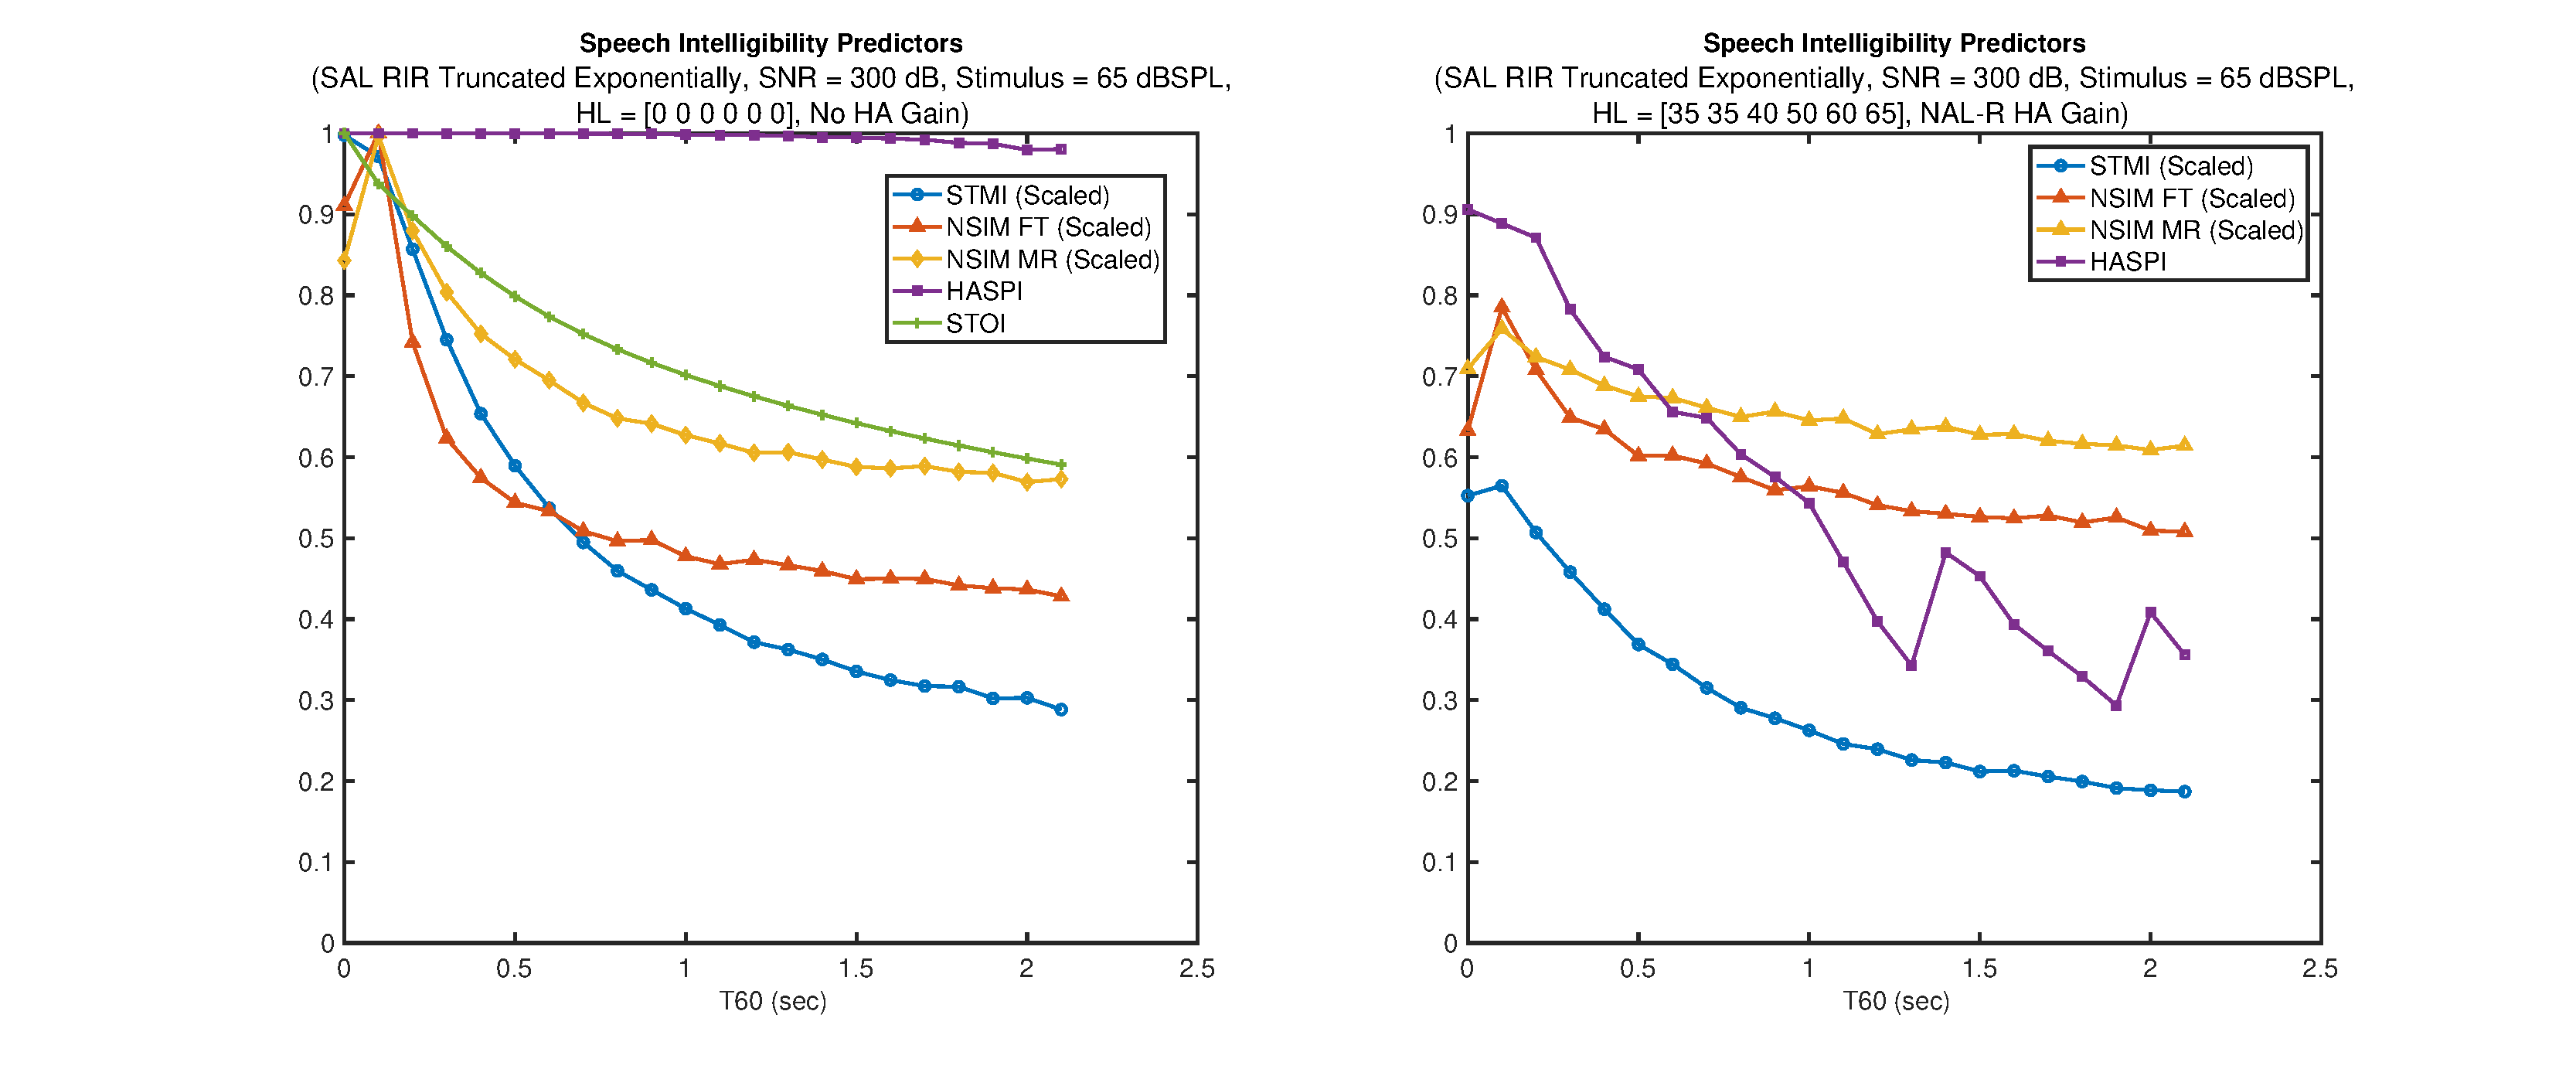
\includegraphics[width=0.98\textwidth]{SIMetricsEval_TruncatedSAL_wScaling}
	\centering
	\caption{Impact of practical reverberation (SAL room from MYRiAD database exponentially truncated to control T60) on SI predictors with and without hearing loss. NAL-R linear hearing aid amplification included in hearing loss case for metrics that including modeling of hearing loss.  Scaling applied to NSIM and STMI values to better view all metrics on the same plot.}
	\label{fig:SIMetricsEval_TruncatedSAL_wScaling}
\end{figure}

\section{Final Method Used}

%\begin{sidewaysfigure}[H]
%	\includegraphics[height=0.9\textheight]{ThesisExperimentMethod}
%	\centering
%	\caption{Block diagram for method used in evaluating dereverberation algorithm performance. Microphone signals include reverberant speech (MYRiAD SAL RIR windowed exponentially to control T60) with added noise signal (real multichannel noise recordings) and added reverberant interference signal. All SI and SQ predictors were computed for the unprocessed microphone signals and the dereverberation output both with and without hearing loss included in all models of speech perception.}
%	\label{fig:Evaluation_Block_Diagram}
%\end{sidewaysfigure}

\begin{sidewaysfigure}
	\includegraphics[width=\columnwidth]{ThesisExperimentMethod}%
	\label{fig:Evaluation_Block_Diagram}
	\caption{Block diagram for method used in evaluating dereverberation algorithm performance. Microphone signals include reverberant speech (MYRiAD SAL RIR windowed exponentially to control T60) with added noise signal (real multichannel noise recordings) and added reverberant interference signal. All SI and SQ predictors were computed for the unprocessed microphone signals and the dereverberation output both with and without hearing loss included in all models of speech perception.}
\end{sidewaysfigure}




\section{Delay-and-Predict Dereverberation Evaluation with Synthetic Reverberation}

\textbf{SI/SQ/Clarity v T60 w/ no noise}

\begin{figure}[H]
	\centering
	\begin{subfigure}[b]{0.47\textwidth}
		\centering
		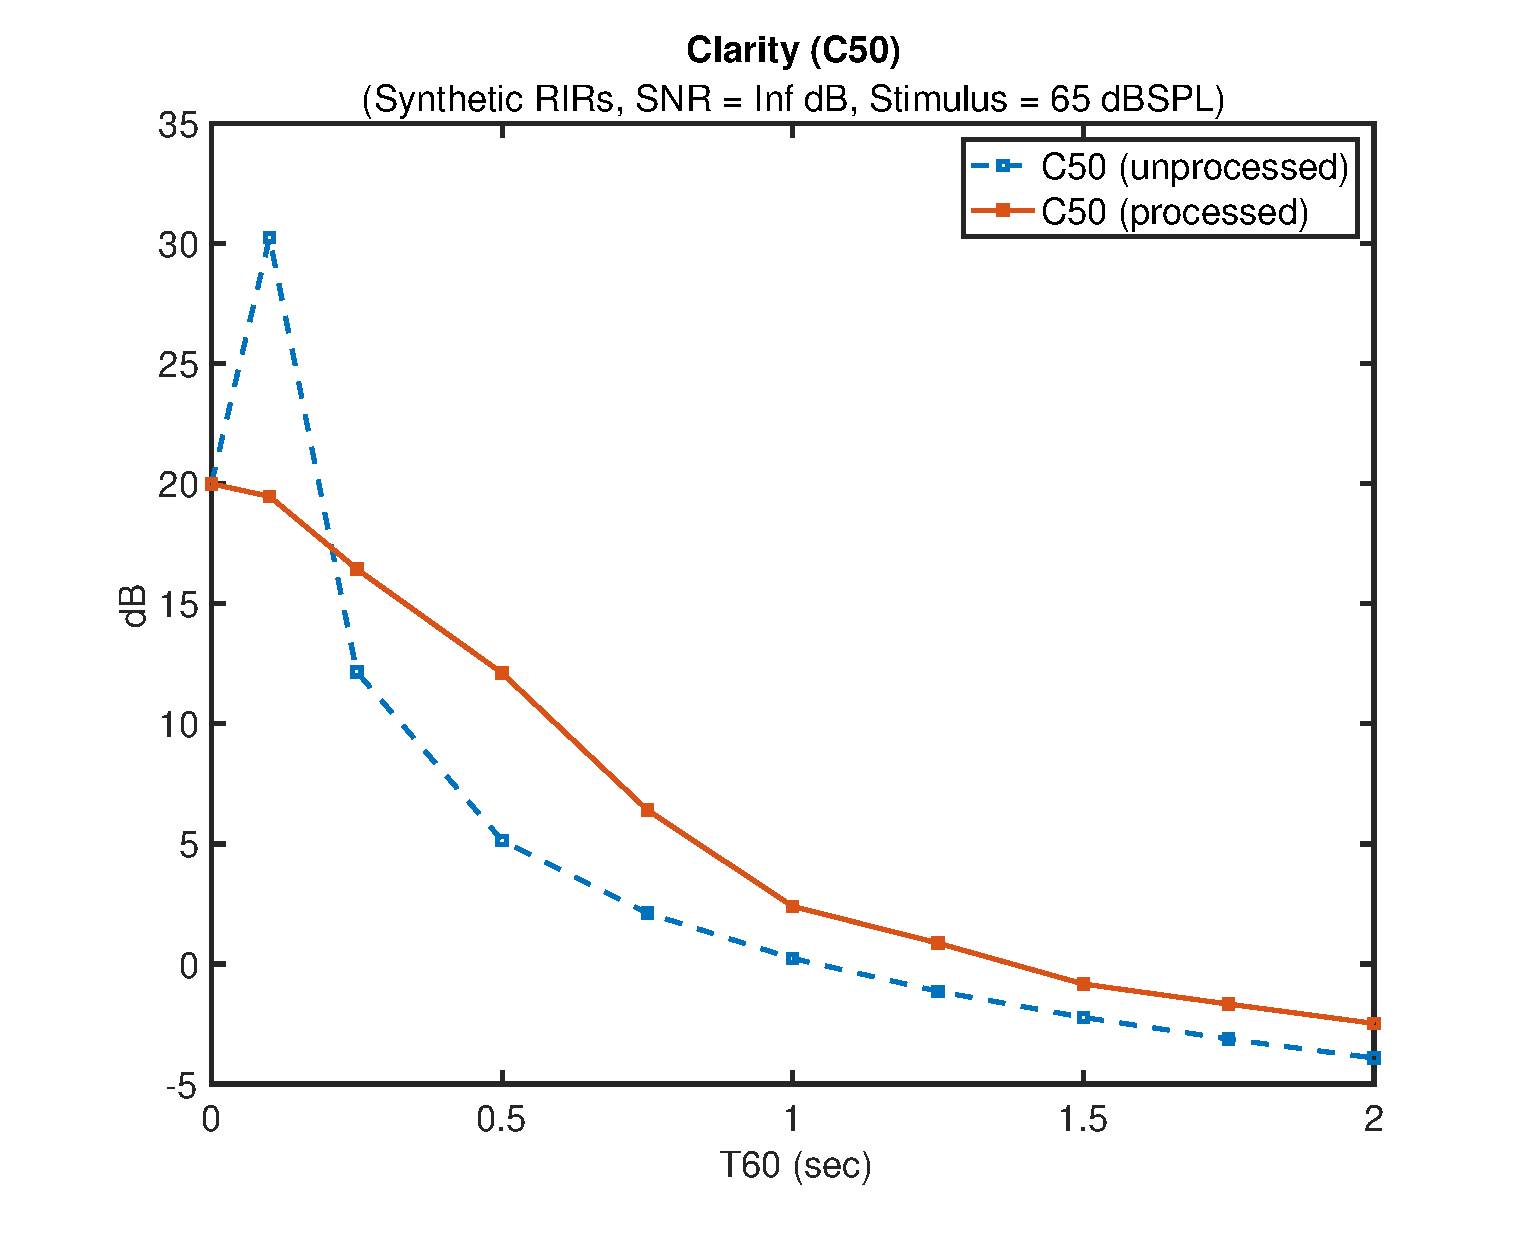
\includegraphics[width=\textwidth]{DAP_EvalT60Sweep_Synthetic_NoNoise_C50_v_T60}
	\end{subfigure}
	\begin{subfigure}[b]{0.92\textwidth}
		\centering
		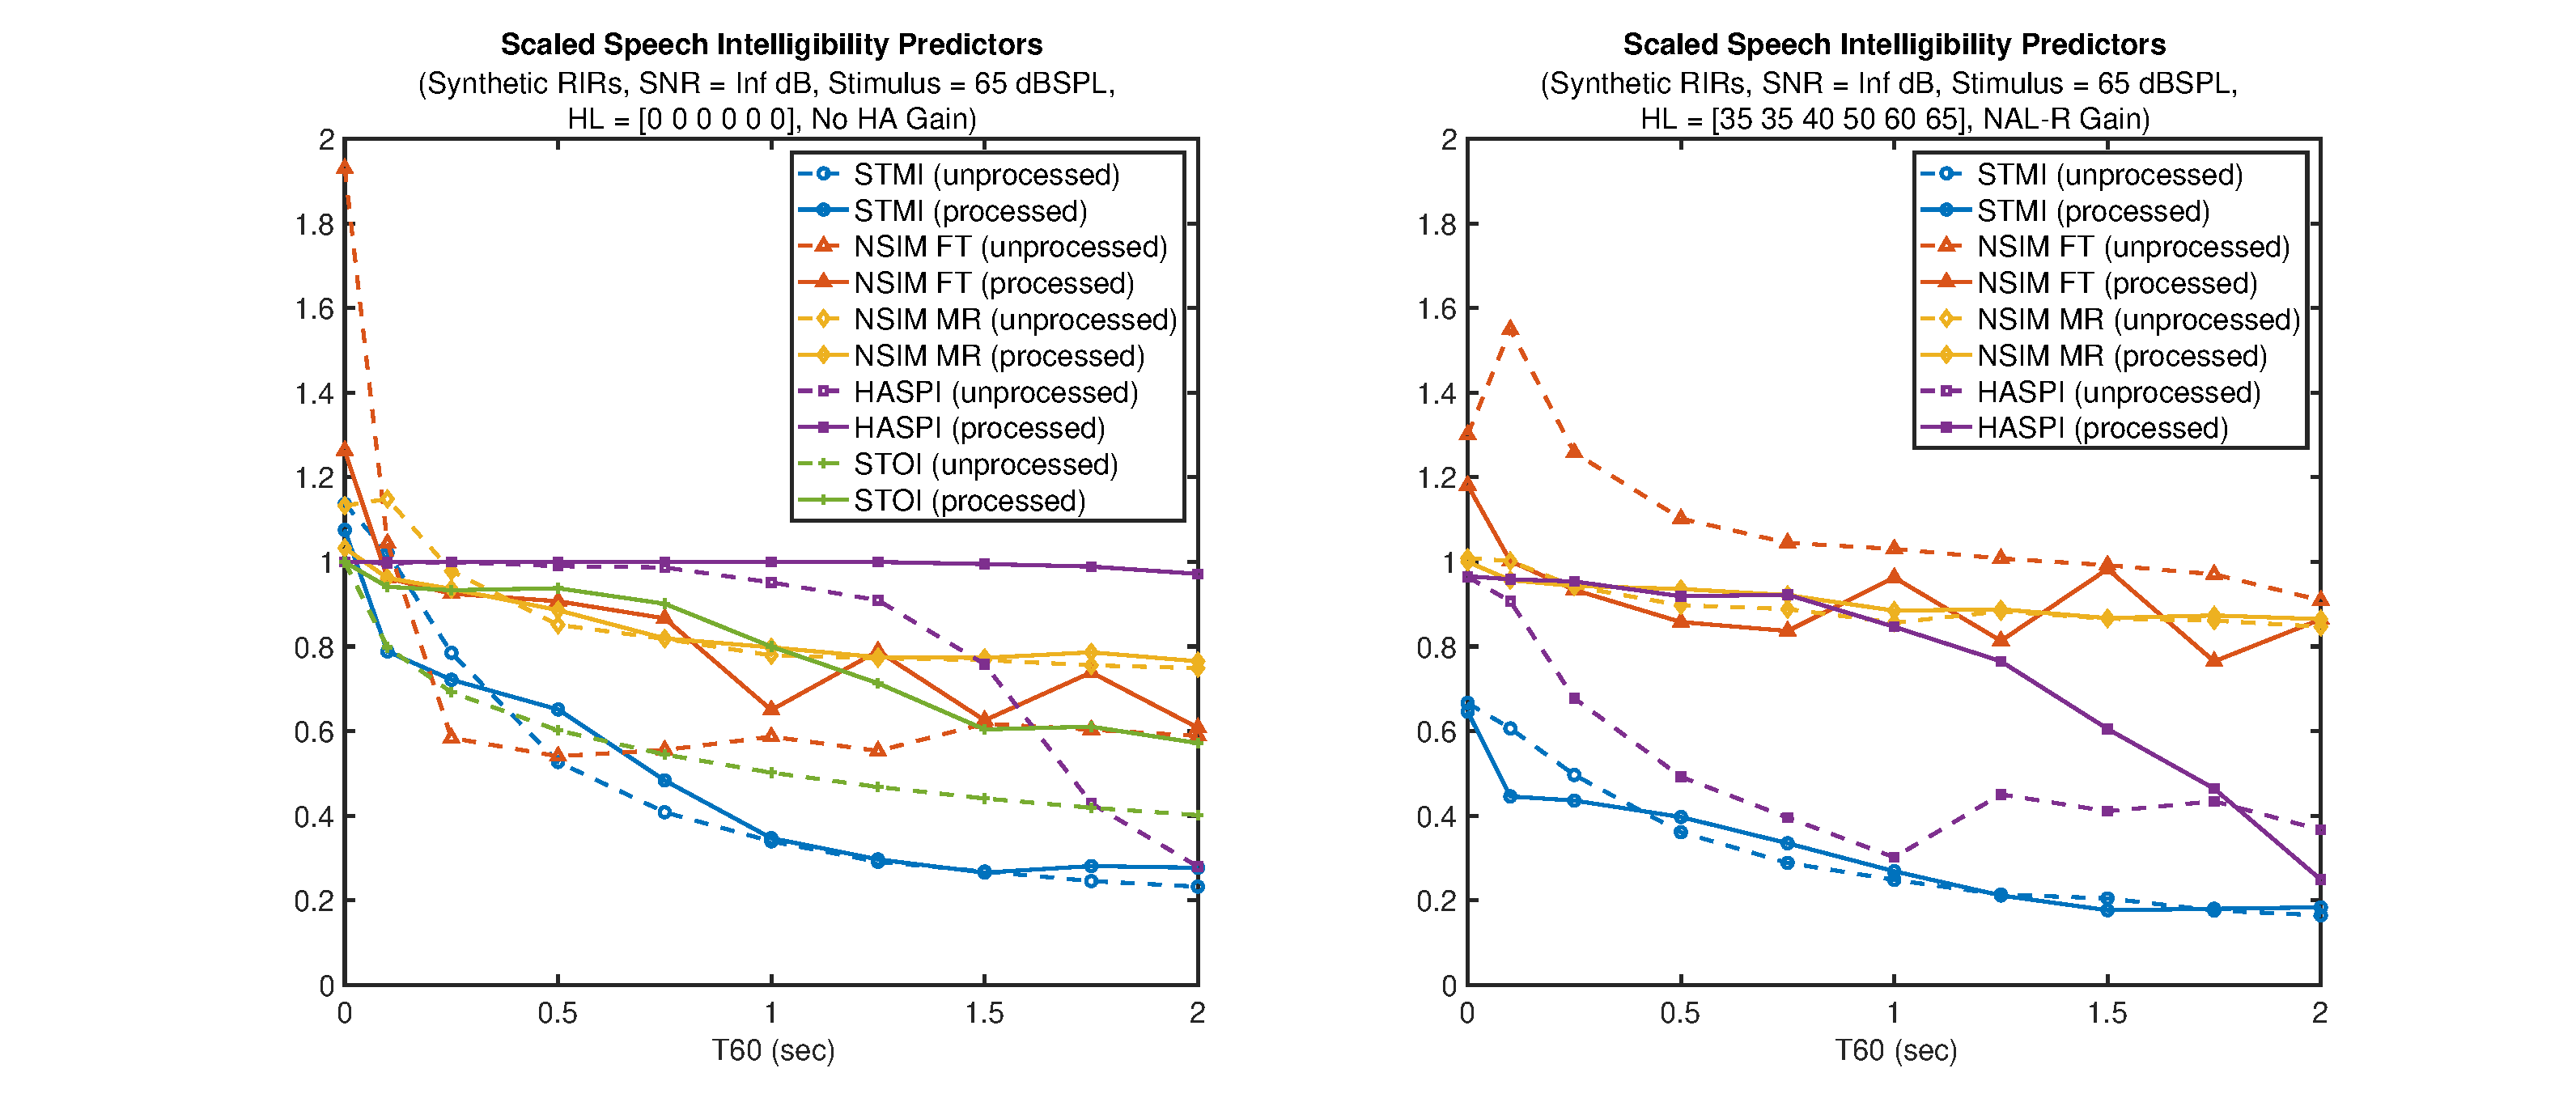
\includegraphics[width=\textwidth]{DAP_EvalT60Sweep_Synthetic_NoNoise_SI_v_T60}
	\end{subfigure}
	\begin{subfigure}[b]{0.92\textwidth}
		\centering
		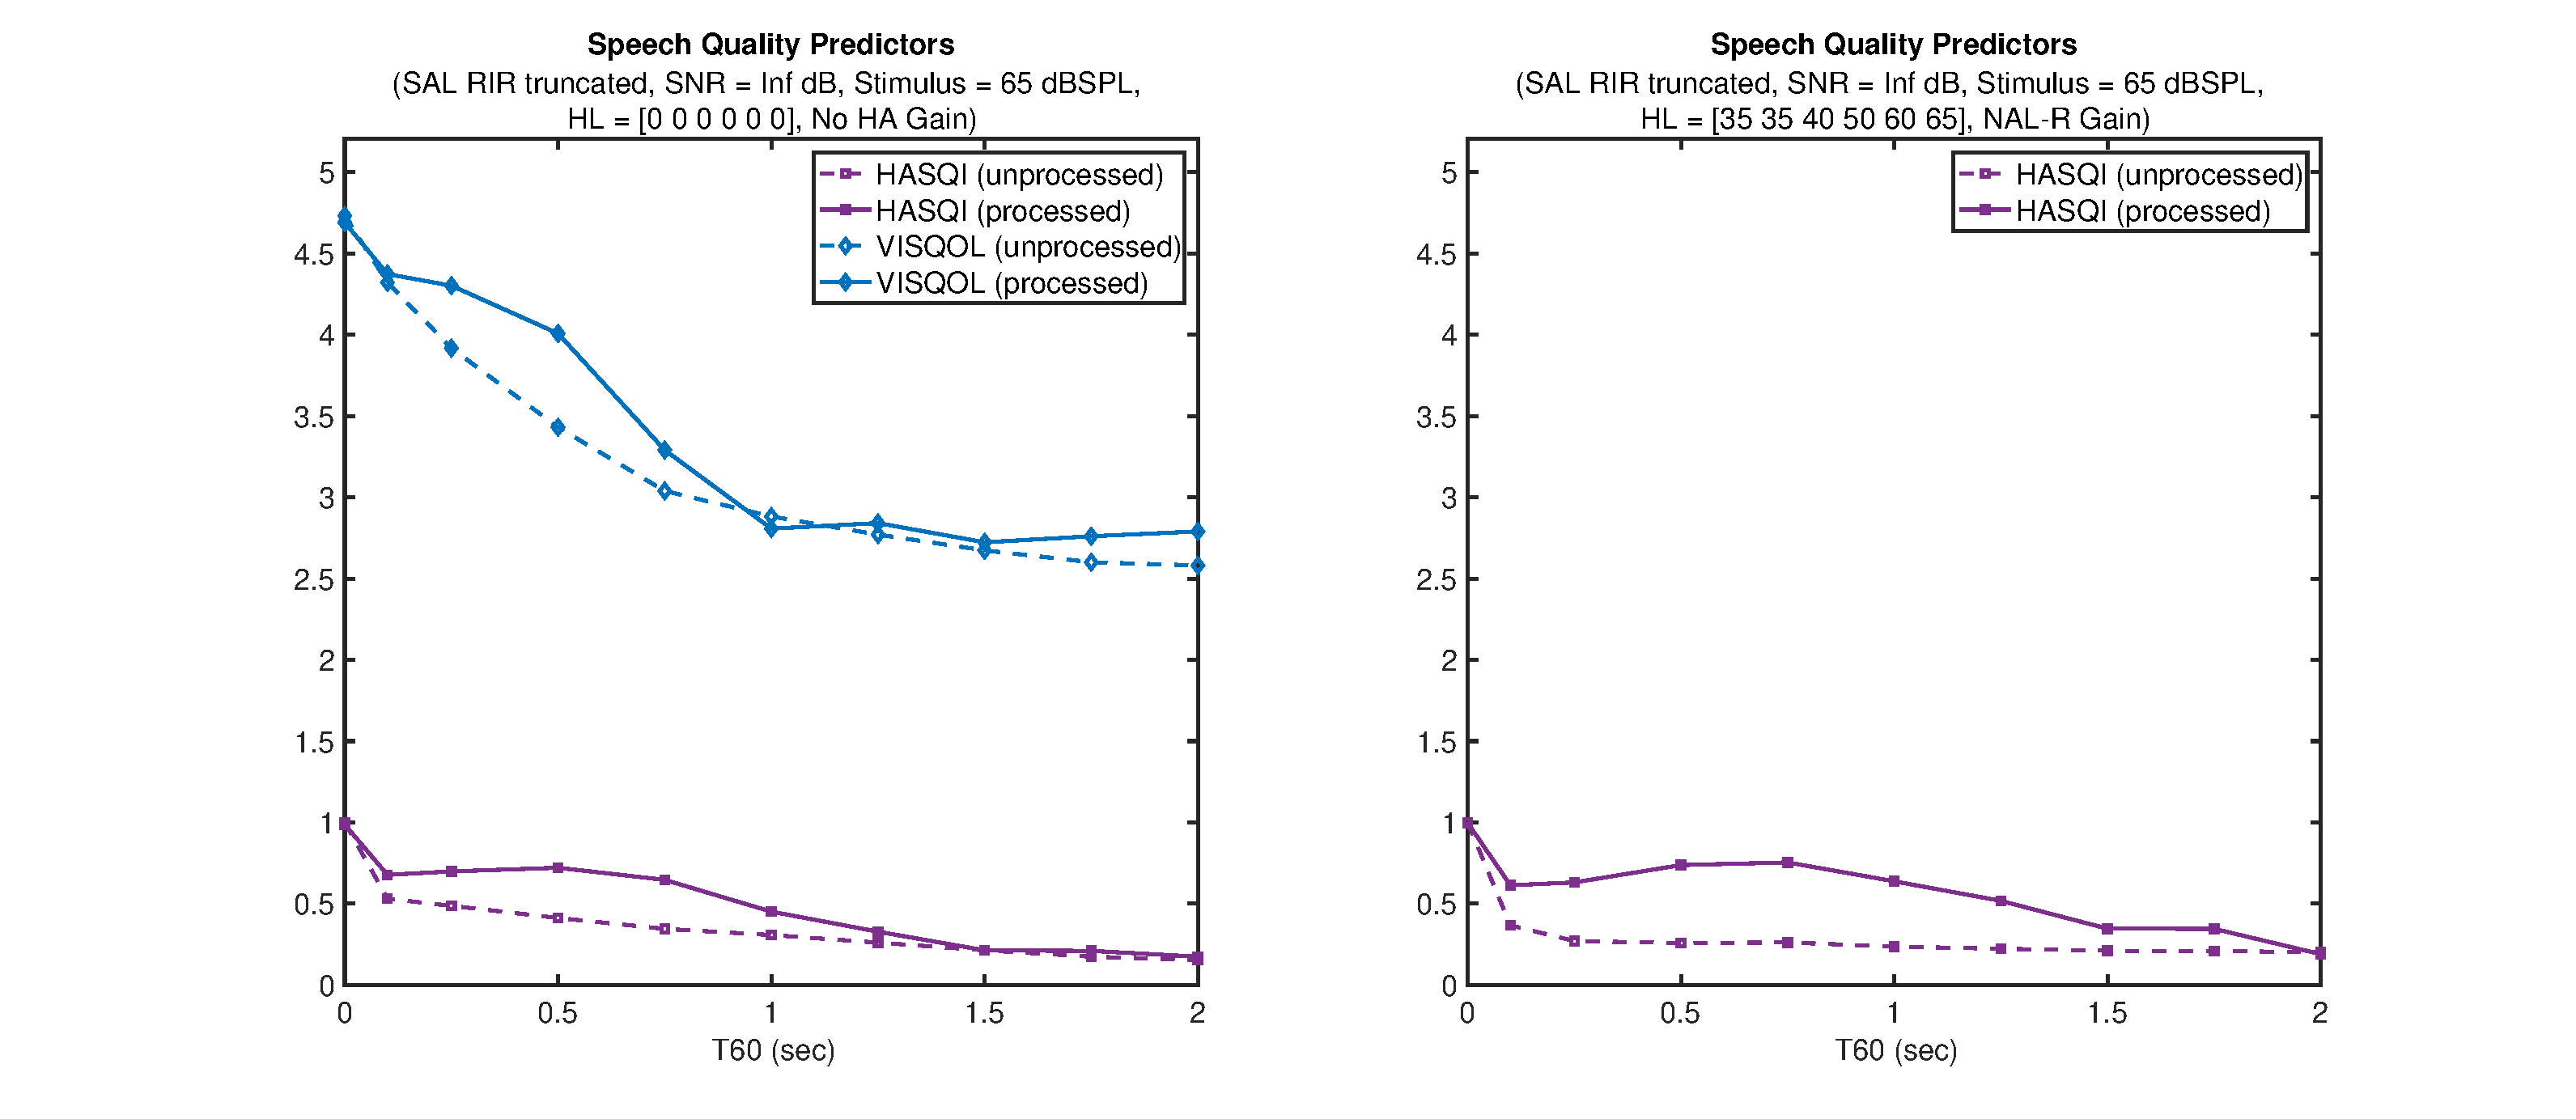
\includegraphics[width=\textwidth]{DAP_EvalT60Sweep_Synthetic_NoNoise_SQ_v_T60}
	\end{subfigure}
	\caption{Evaluation of delay-and-predict dereverberation performance as a function of T60. RIRs were synthetically generated by applying a variable decay-rate exponential window to sequences of uncorrelated Gaussian white noise.}
	\label{fig:DAP_EvalT60Sweep_Synthetic_NoNoise}
\end{figure}

\section{Delay-and-Predict Dereverberation Evaluation with Realistic Reverberation}

\textbf{SI/SQ/Clarity v T60 w/ no noise}

\begin{figure}[H]
	\centering
	\begin{subfigure}[b]{0.47\textwidth}
		\centering
		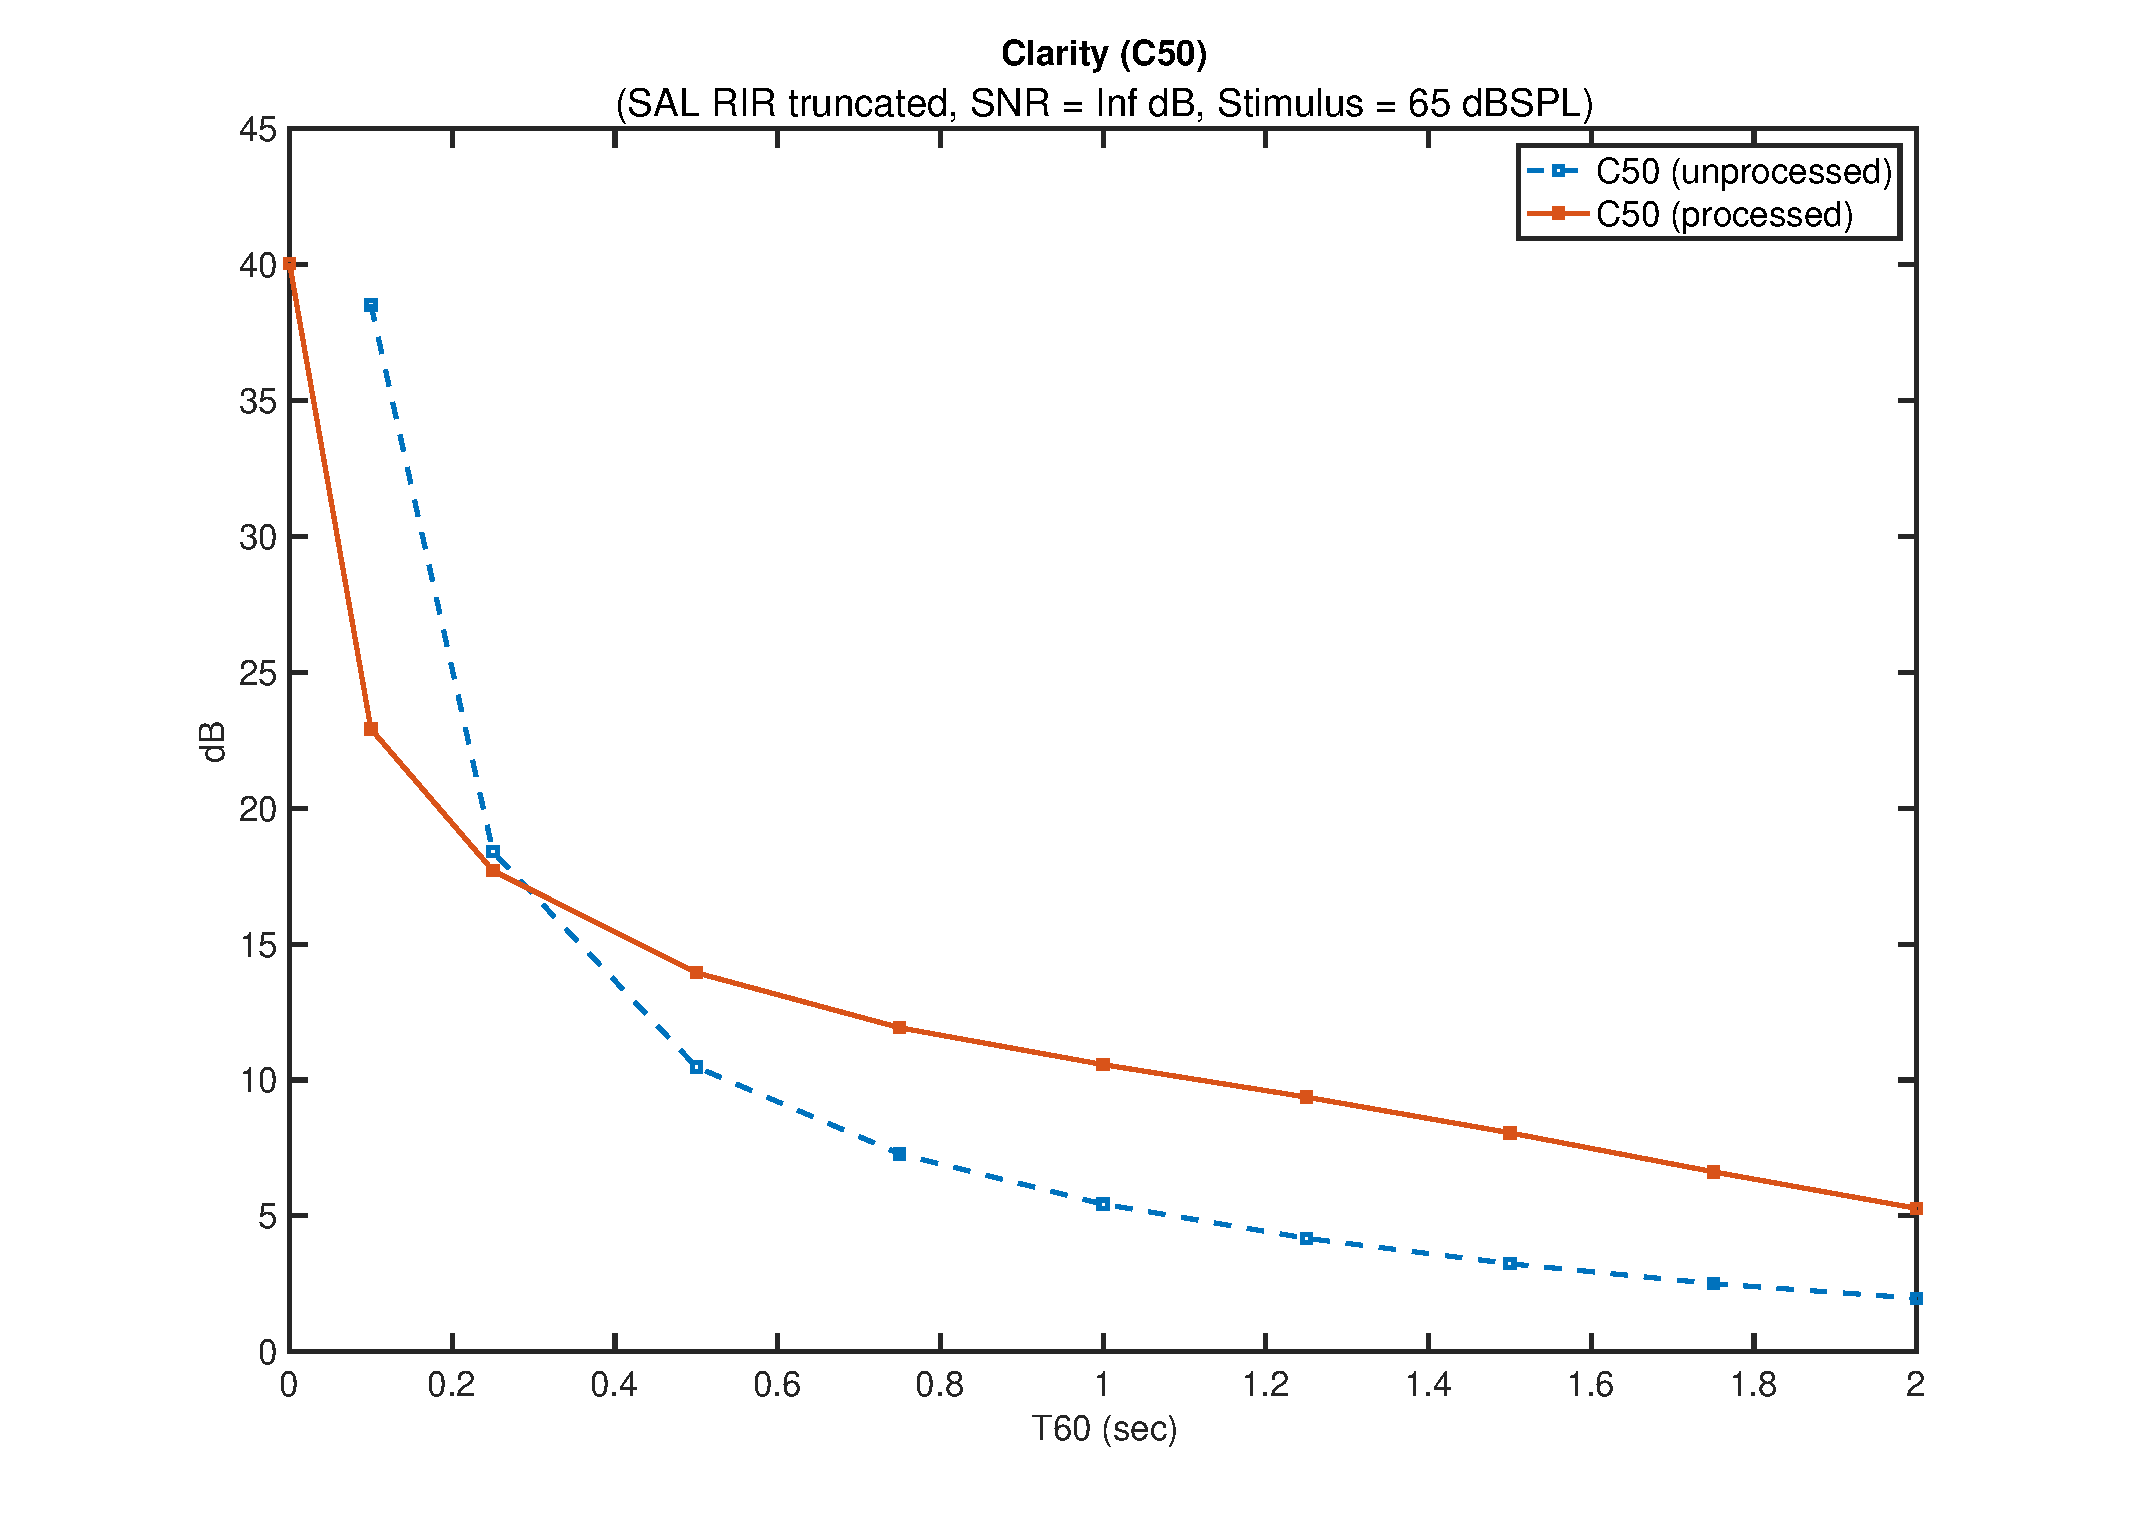
\includegraphics[width=\textwidth]{DAP_EvalT60Sweep_TruncatedSAL_NoNoise_C50_v_T60}
	\end{subfigure}
	\begin{subfigure}[b]{0.92\textwidth}
		\centering
		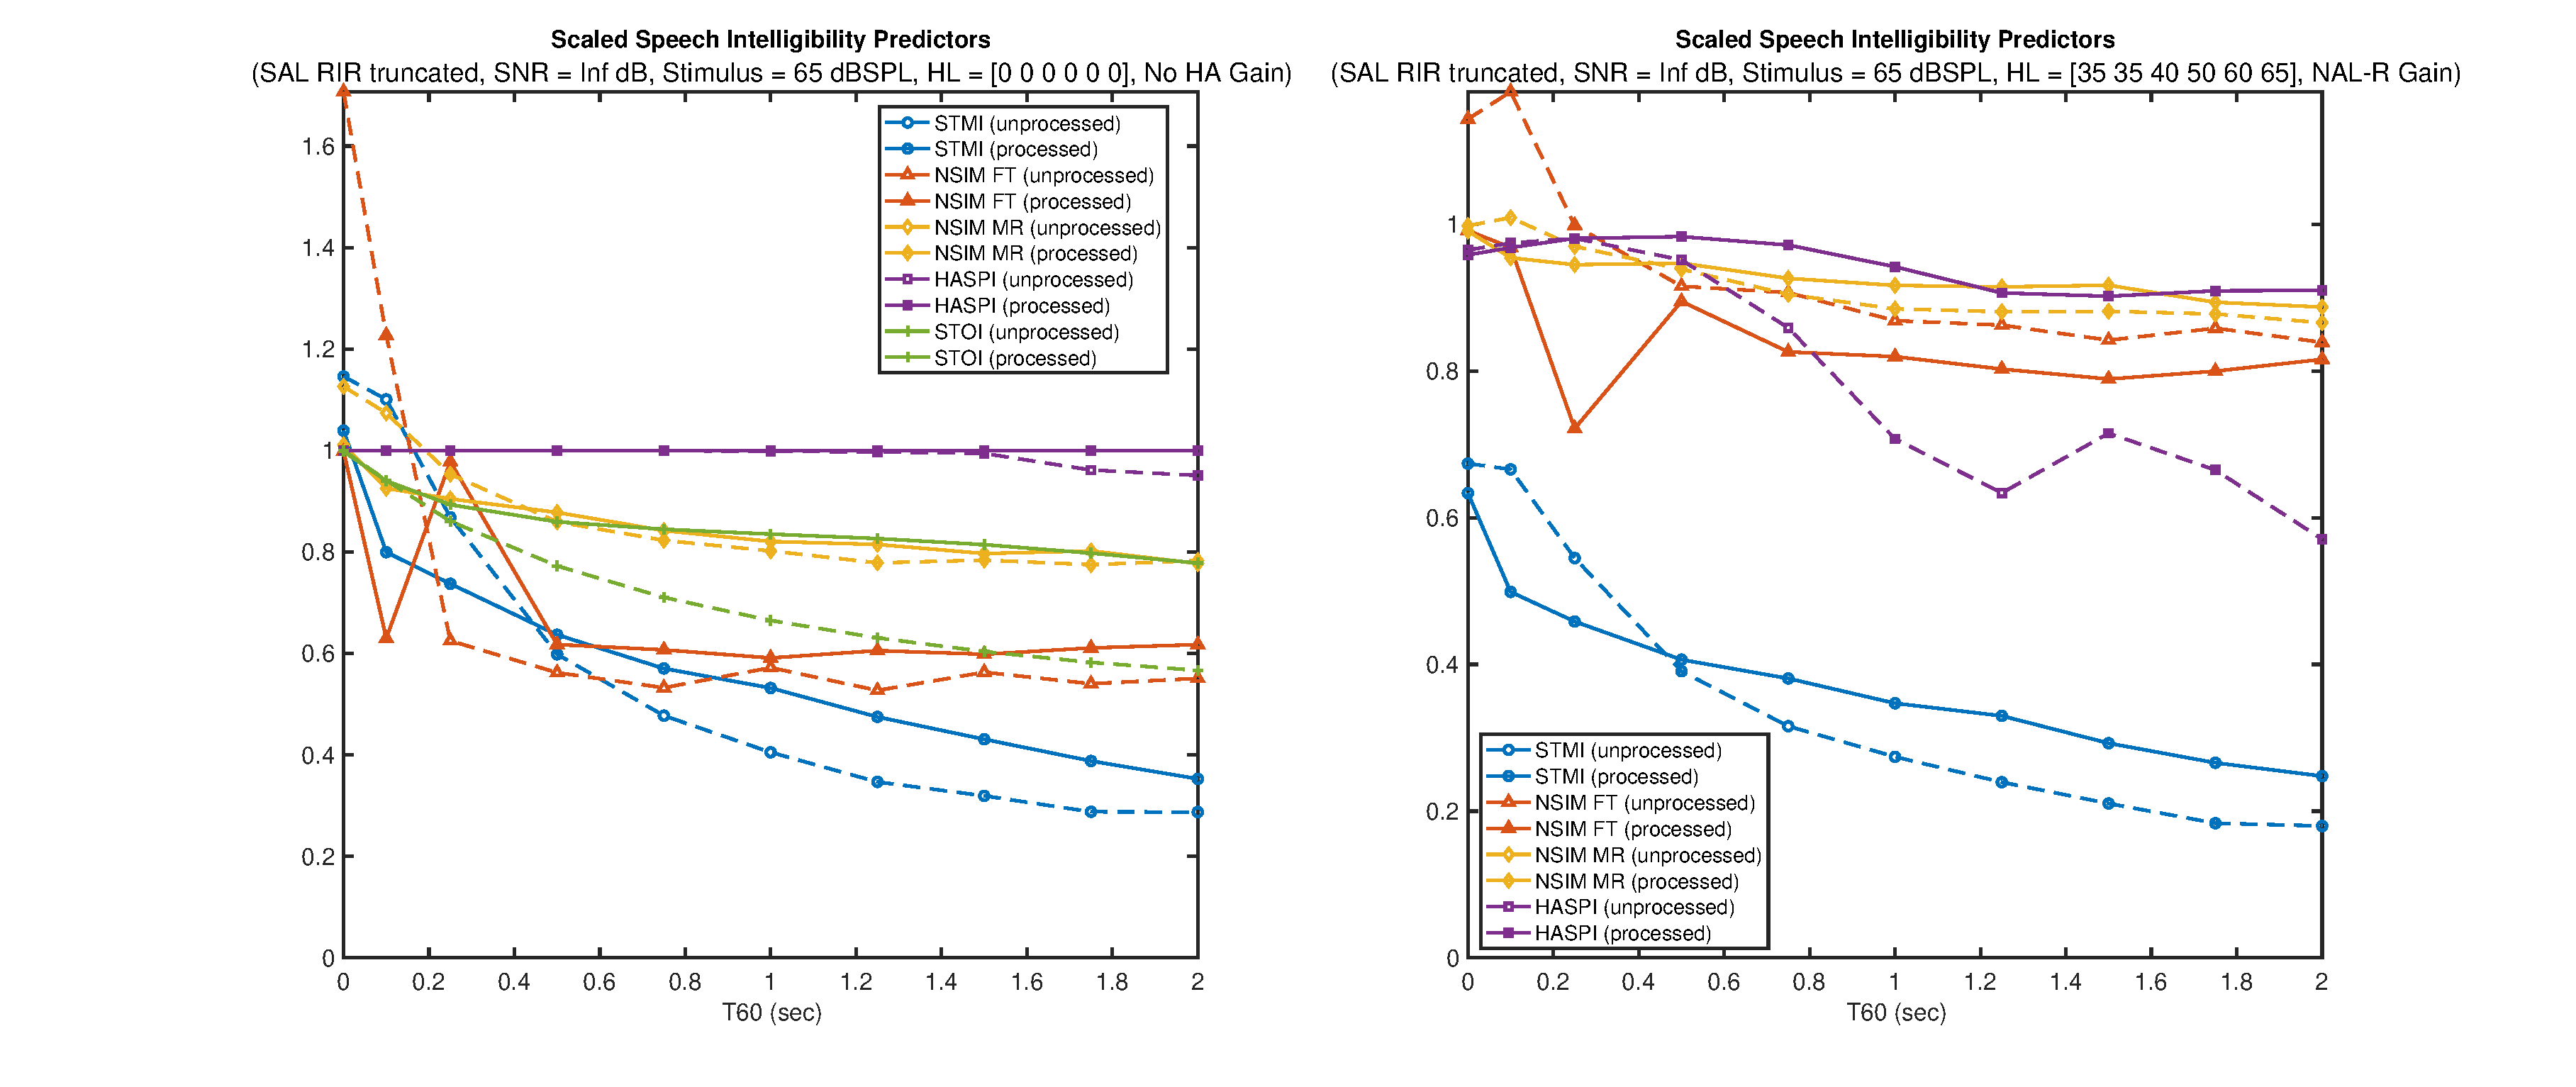
\includegraphics[width=\textwidth]{DAP_EvalT60Sweep_TruncatedSAL_NoNoise_SI_v_T60}
	\end{subfigure}
	\begin{subfigure}[b]{0.92\textwidth}
		\centering
		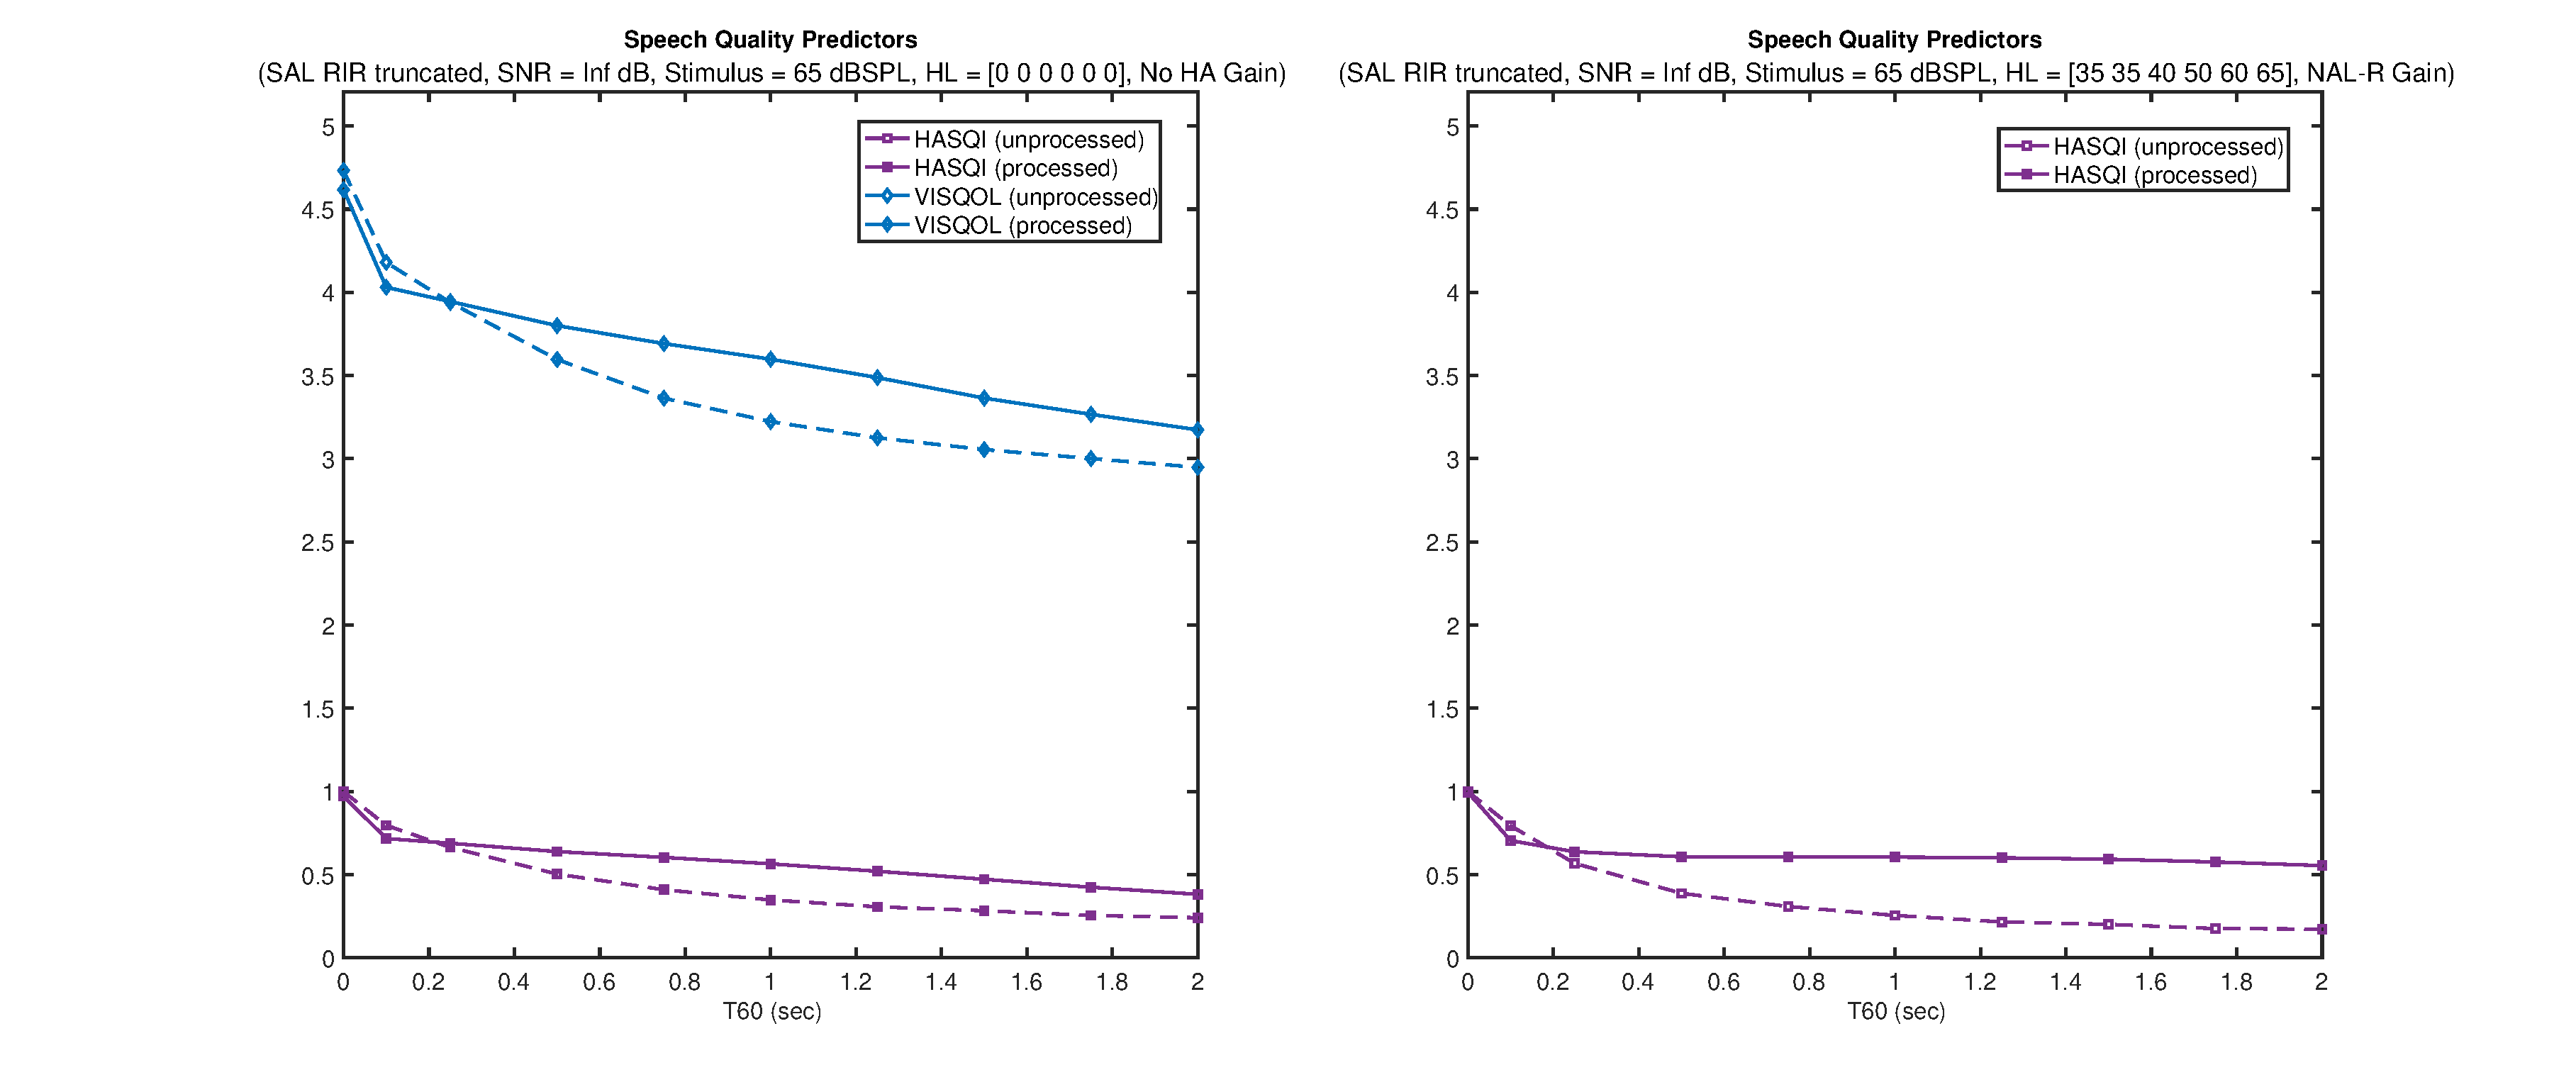
\includegraphics[width=\textwidth]{DAP_EvalT60Sweep_TruncatedSAL_NoNoise_SQ_v_T60}
	\end{subfigure}
	\caption{Evaluation of delay-and-predict dereverberation performance as a function of T60. RIRs were generated by applying a variable decay-rate exponential window to a measured RIR (The SAL room from the MYRiAD database, T60 = 2.2 sec) to control T60.}
	\label{fig:DAP_EvalT60Sweep_TruncatedSAL_NoNoise}
\end{figure}


\section{Impact of Noise on Performance}

\textbf{NOTE: metrics computed on dereverberated speech with noise removed to  neglect the impact of noise on perception (only looking at impacts of reverberation)}

\textbf{SI/SQ/Clarity v T60 w/ SNR = [0 or 12] dB depending on whats needed to show cost}


\begin{figure}[H]
	\centering
	\begin{subfigure}[b]{0.47\textwidth}
		\centering
		\includegraphics[width=\textwidth]{DAP_EvalT60Sweep_TruncatedSAL_SNR12dB_C50_v_T60}
	\end{subfigure}
	\begin{subfigure}[b]{0.92\textwidth}
		\centering
		\includegraphics[width=\textwidth]{DAP_EvalT60Sweep_TruncatedSAL_SNR12dB_SI_v_T60}
	\end{subfigure}
	\begin{subfigure}[b]{0.92\textwidth}
		\centering
		\includegraphics[width=\textwidth]{DAP_EvalT60Sweep_TruncatedSAL_SNR12dB_SQ_v_T60}
	\end{subfigure}
	\caption{Evaluation of delay-and-predict dereverberation performance in the presence of noise as a function of T60. RIRs were generated by applying a variable decay-rate exponential window to a measured RIR (The SAL room from the MYRiAD database, T60 = 2.2 sec) to control T60. Noise was a multichannel recording of approximately stationary noise (Office ventillation noise from the HRIR database), and SNR was set to 12 dB.}
	\label{fig:DAP_EvalT60Sweep_TruncatedSAL_SNR12dB}
\end{figure}

\textbf{SI/SQ/Clarity v SNR w/ T60 = 1 second, stationary noise}

\begin{figure}[H]
	\centering
	\begin{subfigure}[b]{0.47\textwidth}
		\centering
		\includegraphics[width=\textwidth]{DAP_EvalSNRSweepStationary_TruncatedSAL_1000T60_C50_v_SNR}
	\end{subfigure}
	\begin{subfigure}[b]{0.92\textwidth}
		\centering
		\includegraphics[width=\textwidth]{DAP_EvalSNRSweepStationary_TruncatedSAL_1000T60_SI_v_SNR}
	\end{subfigure}
	\begin{subfigure}[b]{0.92\textwidth}
		\centering
		\includegraphics[width=\textwidth]{DAP_EvalSNRSweepStationary_TruncatedSAL_1000T60_SQ_v_SNR}
	\end{subfigure}
	\caption{Evaluation of delay-and-predict dereverberation performance in the presence of noise as a function of SNR. RIRs were generated by applying a variable decay-rate exponential window to a measured RIR (The SAL room from the MYRiAD database, T60 = 2.2 sec) to set T60 = 1 second. Noise was a multichannel recording of approximately stationary noise (Office ventillation noise from the HRIR database).}
	\label{fig:DAP_EvalSNRSweepStationary_TruncatedSAL_1000T60}
\end{figure}

\textbf{SI/SQ/Clarity v SNR w/ T60 = 1 second, Non-Stationary noise}

\begin{figure}[H]
	\centering
	\begin{subfigure}[b]{0.47\textwidth}
		\centering
		\includegraphics[width=\textwidth]{DAP_EvalSNRSweepNonStationary_TruncatedSAL_1000T60_C50_v_SNR}
	\end{subfigure}
	\begin{subfigure}[b]{0.92\textwidth}
		\centering
		\includegraphics[width=\textwidth]{DAP_EvalSNRSweepNonStationary_TruncatedSAL_1000T60_SI_v_SNR}
	\end{subfigure}
	\begin{subfigure}[b]{0.92\textwidth}
		\centering
		\includegraphics[width=\textwidth]{DAP_EvalSNRSweepNonStationary_TruncatedSAL_1000T60_SQ_v_SNR}
	\end{subfigure}
	\caption{Evaluation of delay-and-predict dereverberation performance in the presence of noise as a function of SNR. RIRs were generated by applying a variable decay-rate exponential window to a measured RIR (The SAL room from the MYRiAD database, T60 = 2.2 sec) to set T60 = 1 second. Noise was a multichannel recording of non-stationary noise (Cafeteria babble noise from the HRIR database).}
	\label{fig:DAP_EvalSNRSweepNonStationary_TruncatedSAL_1000T60}
\end{figure}
\section{Impact of an Interfering Talker on Performance}

\textbf{NOTE: metrics computed on dereverberated speech with interfering talker removed to  neglect the impact of interfering talker on perception (only looking at impacts of reverberation on primary talker)}

\textbf{SI/SQ/Clarity v T60 w/ SNR = [0 or 12] dB depending on whats needed to show cost}


\begin{figure}[H]
	\centering
	\begin{subfigure}[b]{0.47\textwidth}
		\centering
		\includegraphics[width=\textwidth]{DAP_EvalT60Sweep_TruncatedSAL_SIR12dB_C50_v_T60}
	\end{subfigure}
	\begin{subfigure}[b]{0.92\textwidth}
		\centering
		\includegraphics[width=\textwidth]{DAP_EvalT60Sweep_TruncatedSAL_SIR12dB_SI_v_T60}
	\end{subfigure}
	\begin{subfigure}[b]{0.92\textwidth}
		\centering
		\includegraphics[width=\textwidth]{DAP_EvalT60Sweep_TruncatedSAL_SIR12dB_SQ_v_T60}
	\end{subfigure}
	\caption{Evaluation of delay-and-predict dereverberation performance in the presence of an interfering talker, as a function of T60. RIRs were generated by applying a variable decay-rate exponential window to a measured RIR (The SAL room from the MYRiAD database, T60 = 2.2 sec) to control T60. Similarly, a measured RIR from a different location in the room was exponentially windowed and used for the interfering talker. The primary-to-interfering talker ratio, i.e., signal-to-interference ratio, was set to SIR = 12 dB.}
	\label{fig:DAP_EvalT60Sweep_TruncatedSAL_SIR12dB}
\end{figure}



        \setcounter{figure}{0}
        \setcounter{equation}{0}
        \setcounter{table}{0}


 \appendix

\chapter{Additional Figures}

\section{Chapter 3 Additional Figures}

\subsection{MC-LP Order} \label{section:appendix:params_p2}

%\textbf{p2 = L / (M-1)  (MINT based on RIR length)}

\begin{figure}[H]
	\centering
	\begin{subfigure}[b]{0.32\textwidth}
		\centering
		\includegraphics[width=\textwidth]{Equalized_RTF_L_div_M_minus_1}
		\subcaption{test} \label{subfig:test_subfig_1}
	\end{subfigure}
	\hfill
	\begin{subfigure}[b]{0.32\textwidth}
		\centering
		\includegraphics[width=\textwidth]{EIR_L_div_M_minus_1}
	\end{subfigure}
	\hfill
	\begin{subfigure}[b]{0.32\textwidth}
		\centering
		\includegraphics[width=\textwidth]{EDC_L_div_M_minus_1}
	\end{subfigure}
	\hfill
	\caption[Detailed behaviour of DAP with $p_2 = L/\left(M-1\right)$]{Delay-and-Predict dereverberation performance with multichannel linear prediction order $\mathrm{p2} = L / (M-1)$, where $L$ is the FIR RIR length and $M$ is the number of channels. Figure \ref{fig:params_p2_stage1} shows the common source whitening filter used.}
	\label{fig:params_p2_L}
\end{figure}

%\textbf{p2 = N60 / (M-1)  (MINT based on T60)}

\begin{figure}[H]
	\centering
	%\begin{subfigure}[b]{0.49\textwidth}
	%	\centering
	%	\includegraphics[width=\textwidth]{S1_N60_div_M_minus_1}
	%\end{subfigure}
	%\hfill
	\begin{subfigure}[b]{0.32\textwidth}
		\centering
		\includegraphics[width=\textwidth]{Equalized_RTF_N60_div_M_minus_1}
	\end{subfigure}
	\hfill
	\begin{subfigure}[b]{0.32\textwidth}
		\centering
		\includegraphics[width=\textwidth]{EIR_N60_div_M_minus_1}
	\end{subfigure}
	\hfill
	\begin{subfigure}[b]{0.32\textwidth}
		\centering
		\includegraphics[width=\textwidth]{EDC_N60_div_M_minus_1}
	\end{subfigure}
	\hfill
	\caption[Detailed behaviour of DAP with $p_2 = N60/\left(M-1\right)$]{Delay-and-Predict dereverberation performance with multichannel linear prediction order $\mathrm{p2} = \mathrm{N60} / (M-1)$, where N60 is the number of samples corresponding to the T60 and $M$ is the number of channels (i.e., the MINT condition based on T60 rather than the FIR RIR length). Figure \ref{fig:params_p2_stage1} shows the common source whitening filter used.}
	\label{fig:params_p2_N60}
\end{figure}

%\textbf{p2 = 0p75 * N60 / (M-1) (Suboptimal)}

\begin{figure}[H]
	\centering
	%\begin{subfigure}[b]{0.49\textwidth}
	%	\centering
	%	\includegraphics[width=\textwidth]{S1_0p75N60_div_M_minus_1}
	%\end{subfigure}
	%\hfill
	\begin{subfigure}[b]{0.32\textwidth}
		\centering
		\includegraphics[width=\textwidth]{Equalized_RTF_0p75N60_div_M_minus_1}
	\end{subfigure}
	\hfill
	\begin{subfigure}[b]{0.32\textwidth}
		\centering
		\includegraphics[width=\textwidth]{EIR_0p75N60_div_M_minus_1}
	\end{subfigure}
	\hfill
	\begin{subfigure}[b]{0.32\textwidth}
		\centering
		\includegraphics[width=\textwidth]{EDC_0p75N60_div_M_minus_1}
	\end{subfigure}
	\hfill
	\caption[Detailed behaviour of DAP with $p_2 = 0.75 \cdot N60/\left(M-1\right)$]{Delay-and-Predict dereverberation performance with multichannel linear prediction order $\mathrm{p2} = 0.75 \cdot \mathrm{N60} / (M-1)$, where N60 is the number of samples corresponding to the T60 and $M$ is the number of channels (i.e., suboptimal with respect to the MINT condition based on T60 rather than the FIR RIR length). Figure \ref{fig:params_p2_stage1} shows the common source whitening filter used.}
	\label{fig:params_p2_0p75_N60}
\end{figure}

%\textbf{p2 = 0.5 * N60 / (M-1) (More suboptimal)}

\begin{figure}[H]
	\centering
	%\begin{subfigure}[b]{0.49\textwidth}
	%	\centering
	%	\includegraphics[width=\textwidth]{S1_0p5N60_div_M_minus_1}
	%\end{subfigure}
	%\hfill
	\begin{subfigure}[b]{0.32\textwidth}
		\centering
		\includegraphics[width=\textwidth]{Equalized_RTF_0p5N60_div_M_minus_1}
	\end{subfigure}
	\hfill
	\begin{subfigure}[b]{0.32\textwidth}
		\centering
		\includegraphics[width=\textwidth]{EIR_0p5N60_div_M_minus_1}
	\end{subfigure}
	\hfill
	\begin{subfigure}[b]{0.32\textwidth}
		\centering
		\includegraphics[width=\textwidth]{EDC_0p5N60_div_M_minus_1}
	\end{subfigure}
	\hfill
	\caption[Detailed behaviour of DAP with $p_2 = 0.5 \cdot N60/\left(M-1\right)$]{Delay-and-Predict dereverberation performance with multichannel linear prediction order $\mathrm{p2} = 0.5 \cdot \mathrm{N60} / (M-1)$, where N60 is the number of samples corresponding to the T60 and $M$ is the number of channels (i.e., More suboptimal with respect to the MINT condition based on T60 rather than the FIR RIR length). Figure \ref{fig:params_p2_stage1} shows the common source whitening filter used.}
	\label{fig:params_p2_0p5_N60}
\end{figure}

\subsection{Source Whitening Order} \label{section:appendix:params_p1}

%\textbf{p1 = 200 (Original Paper)}

\begin{figure}[H]
	\centering
	\begin{subfigure}[b]{0.49\textwidth}
		\centering
		\includegraphics[width=\textwidth]{S1_p1_200}
	\end{subfigure}
	\hfill
	\begin{subfigure}[b]{0.49\textwidth}
		\centering
		\includegraphics[width=\textwidth]{Equalized_RTF_p1_200}
	\end{subfigure}
	\hfill
	\begin{subfigure}[b]{0.49\textwidth}
		\centering
		\includegraphics[width=\textwidth]{EIR_p1_200}
	\end{subfigure}
	\hfill
	\begin{subfigure}[b]{0.49\textwidth}
		\centering
		\includegraphics[width=\textwidth]{EDC_p1_200}
	\end{subfigure}
	\hfill
	\caption[Detailed behaviour of DAP with $p_1 = 200$]{Delay-and-Predict dereverberation performance with source whitening prediction order $\mathrm{p1} = 200$ and multichannel linear prediction order $\mathrm{p2} = \mathrm{N60}  / (M-1)$.}
	\label{fig:params_p1_200}
\end{figure}

%\textbf{p1 = 1000}

\begin{figure}[H]
	\centering
	\begin{subfigure}[b]{0.49\textwidth}
		\centering
		\includegraphics[width=\textwidth]{S1_p1_1000}
	\end{subfigure}
	\hfill
	\begin{subfigure}[b]{0.49\textwidth}
		\centering
		\includegraphics[width=\textwidth]{Equalized_RTF_p1_1000}
	\end{subfigure}
	\hfill
	\begin{subfigure}[b]{0.49\textwidth}
		\centering
		\includegraphics[width=\textwidth]{EIR_p1_1000}
	\end{subfigure}
	\hfill
	\begin{subfigure}[b]{0.49\textwidth}
		\centering
		\includegraphics[width=\textwidth]{EDC_p1_1000}
	\end{subfigure}
	\hfill
	\caption[Detailed behaviour of DAP with $p_1 = 1000$]{Delay-and-Predict dereverberation performance with source whitening prediction order $\mathrm{p1} = 1000$ and multichannel linear prediction order $\mathrm{p2} = \mathrm{N60} / (M-1)$.}
	\label{fig:params_p1_1000}
\end{figure}

%\textbf{p1 = p2 * (M-1) (whitened on the same spectral resolution as the MC-LP equalizer)}

\begin{figure}[H]
	\centering
	\begin{subfigure}[b]{0.49\textwidth}
		\centering
		\includegraphics[width=\textwidth]{S1_p1_based_on_p2}
	\end{subfigure}
	\hfill
	\begin{subfigure}[b]{0.49\textwidth}
		\centering
		\includegraphics[width=\textwidth]{Equalized_RTF_p1_based_on_p2}
	\end{subfigure}
	\hfill
	\begin{subfigure}[b]{0.49\textwidth}
		\centering
		\includegraphics[width=\textwidth]{EIR_p1_based_on_p2}
	\end{subfigure}
	\hfill
	\begin{subfigure}[b]{0.49\textwidth}
		\centering
		\includegraphics[width=\textwidth]{EDC_p1_based_on_p2}
	\end{subfigure}
	\hfill
	\caption[Detailed behaviour of DAP with $p_1 = p_2 \cdot \left(M-1\right)$]{Delay-and-Predict dereverberation performance with source whitening prediction order $\mathrm{p1} = \mathrm{p2} \cdot (M-1)$ and multichannel linear prediction order $\mathrm{p2} = \mathrm{N60} / (M-1)$. I.e., The source whitening filter order is the same as the effective MINT filter order.}
	\label{fig:params_p1_based_on_p2}
\end{figure}

%\textbf{p1 = 2 * p2  * (M-1) (Extra headroom)}

\begin{figure}[H]
	\centering
	\begin{subfigure}[b]{0.49\textwidth}
		\centering
		\includegraphics[width=\textwidth]{S1_p1_2x_p2}
	\end{subfigure}
	\hfill
	\begin{subfigure}[b]{0.49\textwidth}
		\centering
		\includegraphics[width=\textwidth]{Equalized_RTF_p1_2x_p2}
	\end{subfigure}
	\hfill
	\begin{subfigure}[b]{0.49\textwidth}
		\centering
		\includegraphics[width=\textwidth]{EIR_p1_2x_p2}
	\end{subfigure}
	\hfill
	\begin{subfigure}[b]{0.49\textwidth}
		\centering
		\includegraphics[width=\textwidth]{EDC_p1_2x_p2}
	\end{subfigure}
	\hfill
	\caption[Detailed behaviour of DAP with $p_1 = 2 \cdot p_2 \cdot \left(M-1\right)$]{Delay-and-Predict dereverberation performance with source whitening prediction order $\mathrm{p1} = 2 \cdot \mathrm{p2} \cdot (M-1)$ and multichannel linear prediction order $\mathrm{p2} = \mathrm{N60} / (M-1)$. I.e., The source whitening filter order is twice the effective MINT filter order.}
	\label{fig:params_p1_2x_p2}
\end{figure}

%... beyond about p1 = 1.25 * p2 * (M-1) EDC performance saturates at approximately -35 dB reverb attenuation.


\section{Chapter 4 Additional Figures}

\subsection{EC Evaluation} \label{section:appendix:EC_eval}


\begin{figure}[H]
	\centering
	\begin{subfigure}[b]{0.49\textwidth}
		\centering
		\includegraphics[width=\textwidth]{EC_SRM_AnechoicSpeech_AnechoicNoise}
	\end{subfigure}
	\hfill
	\begin{subfigure}[b]{0.49\textwidth}
		\centering
		\includegraphics[width=\textwidth]{EC_SRM_AnechoicSpeech_ReverbNoise}
	\end{subfigure}
	\hfill
	\begin{subfigure}[b]{0.49\textwidth}
		\centering
		\includegraphics[width=\textwidth]{EC_SRM_AnechoicSpeech_SpatialNoiseRecording}
	\end{subfigure}
	\hfill
	\begin{subfigure}[b]{0.49\textwidth}
		\centering
		\includegraphics[width=\textwidth]{EC_SRM_AnechoicSpeech_DiffuseNoise}
	\end{subfigure}
	\hfill
	\caption[EC front-end performance with anechoic speech]{Impact of EC algorithm on speech intelligibility (using HASPI) as a function of SNR, for anechoic directional speech and various noise types (anechoic directional, reverberant, spatial recording, diffuse)}
	\label{fig:EC_SRM_AnechoicSpeech}
\end{figure}


\begin{figure}[H]
	\centering
	\begin{subfigure}[b]{0.49\textwidth}
		\centering
		\includegraphics[width=\textwidth]{EC_SRM_ReverbSpeech_AnechoicNoise}
	\end{subfigure}
	\hfill
	\begin{subfigure}[b]{0.49\textwidth}
		\centering
		\includegraphics[width=\textwidth]{EC_SRM_ReverbSpeech_ReverbNoise}
	\end{subfigure}
	\hfill
	\begin{subfigure}[b]{0.49\textwidth}
		\centering
		\includegraphics[width=\textwidth]{EC_SRM_ReverbSpeech_SpatialNoiseRecording}
	\end{subfigure}
	\hfill
	\begin{subfigure}[b]{0.49\textwidth}
		\centering
		\includegraphics[width=\textwidth]{EC_SRM_ReverbSpeech_DiffuseNoise}
	\end{subfigure}
	\hfill
	\caption[EC front-end performance with reverberant speech]{Impact of EC algorithm on speech intelligibility (using HASPI) as a function of SNR, for reverberant speech and various noise types (anechoic directional, reverberant, spatial recording, diffuse)}
	\label{fig:EC_SRM_ReverbSpeech}
\end{figure}


\begin{figure}[H]
	\centering
	\begin{subfigure}[b]{0.49\textwidth}
		\centering
		\includegraphics[width=\textwidth]{EC_SRM_DiffuseSpeech_AnechoicNoise}
	\end{subfigure}
	\hfill
	\begin{subfigure}[b]{0.49\textwidth}
		\centering
		\includegraphics[width=\textwidth]{EC_SRM_DiffuseSpeech_ReverbNoise}
	\end{subfigure}
	\hfill
	\begin{subfigure}[b]{0.49\textwidth}
		\centering
		\includegraphics[width=\textwidth]{EC_SRM_DiffuseSpeech_SpatialNoiseRecording}
	\end{subfigure}
	\hfill
	\begin{subfigure}[b]{0.49\textwidth}
		\centering
		\includegraphics[width=\textwidth]{EC_SRM_DiffuseSpeech_DiffuseNoise}
	\end{subfigure}
	\hfill
	\caption[EC front-end performance with diffuse speech]{Impact of EC algorithm on speech intelligibility (using HASPI) as a function of SNR, for diffuse speech and various noise types (anechoic directional, reverberant, spatial recording, diffuse)}
	\label{fig:EC_SRM_DiffuseSpeech}
\end{figure}

\subsection{Higher Order Delay-and-Predict Dereverberation Evaluation in Variable Reverberation with regularization} \label{section:appendix:DAP_EVAL_1000p2wReg}

\begin{figure}[H]
	\centering
	\begin{subfigure}[b]{0.47\textwidth}
		\centering
		\includegraphics[width=\textwidth]{DAP_EVAL_1000T60max_wReg_C50_v_T60}
	\end{subfigure}
	\begin{subfigure}[b]{0.92\textwidth}
		\centering
		\includegraphics[width=\textwidth]{DAP_EVAL_1000T60max_wReg_SI_v_T60}
	\end{subfigure}
	\begin{subfigure}[b]{0.92\textwidth}
		\centering
		\includegraphics[width=\textwidth]{DAP_EVAL_1000T60max_wReg_SQ_v_T60}
	\end{subfigure}
	\caption[DAP evaluation with regularization and $p_2=2667$]{Evaluation of delay-and-predict dereverberation performance with autocorrelation regularization as a function of T60. Prediction orders were $p_2 = 5333$ and $p_1=20000$ (i.e., according to $T60_{\mathrm{max}} = \qty{1}{\sec}$ for$M=4$ and $f_s=\qty{16}{\kilo\hertz})$. RIRs were generated by applying a variable decay-rate exponential window to a measured RIR (The SAL room from the MYRiAD database, $\mathrm{T60} = \qty{2.2}{\second}$) to control T60. No Noise or Interfering talker were included.}
	\label{fig:DAP_EVAL_1000T60max_wReg}
\end{figure}



               % you can include your appendix if you have any!

\bibliographystyle{natbib}
\bibliography{references}        % your list of references

\label{NumDocumentPages}

\end{document}
% ********************************
